\documentclass[11pt]{article}
% -------------------------------------------- usepackage  -------------------------------------------- %
\usepackage[utf8]{inputenc}
\usepackage[english]{babel}
\usepackage[T1]{fontenc}
\usepackage{amsmath,amssymb,amsfonts}
\usepackage{ulem}
\usepackage{subcaption}
\usepackage{caption}
\usepackage{gauss}
\usepackage{mathtools}
\usepackage{mathrsfs}
\usepackage{hyperref}
\usepackage{bbm}
\usepackage{graphicx} 
\usepackage{enumerate} 
\usepackage{fancyhdr} 
\usepackage{lastpage} 
\usepackage[margin=1in,footskip=0.25in]{geometry}
%\usepackage[a4paper, lmargin=2cm, hmargin=3cm]{geometry}
\usepackage{pdfpages}
\usepackage{pdfpages}
\usepackage{bookmark}
\usepackage{lipsum}
\usepackage{xcolor}
\usepackage{amsthm}
\usepackage{graphicx}
\usepackage{float}
\usepackage{tikz}
\usepackage{booktabs}
\usepackage{pgfplots}
\usepackage{color, colortbl}
\counterwithin{figure}{section}
\counterwithin{table}{section}
\definecolor{Gray}{gray}{0.9}
\definecolor{LightCyan}{rgb}{0.88,1,1}
\numberwithin{equation}{section}
\hypersetup{
    colorlinks=true,
    linkcolor=blue,
    filecolor=magenta,      
    urlcolor=cyan,
}
% -------------------------------------------- newcommand  -------------------------------------------- %
\pagestyle{fancy}
\setcounter{MaxMatrixCols}{20}
\newcommand{\pic}[3]{\makebox[\textwidth]{\textbf{#1}}
\\
\begin{center}
\includegraphics[scale=#2,center]{#3}
\end{center}}
\newcommand{\QQ}{\mathbb{Q}}
\newcommand{\RR}{\mathbb{R}}
\newcommand{\BB}{\mathbb{B}}
\newcommand{\NN}{\mathbb{N}}
\newcommand{\FF}{\mathbb{F}}
\newcommand{\ZZ}{\mathbb{Z}}
\newcommand{\CC}{\mathbb{C}}
\newcommand{\EE}{\mathbb{E}}
\newcommand{\PP}{\mathbb{P}}
\newcommand{\indi}[1]{\mathbbm{1}_{#1}}
\newcommand{\limi}[2]{\liminf\limits_{#1\rightarrow#2}}
\newcommand{\bcup}[1]{\bigcup\limits_{#1}}
\newcommand{\bcap}[1]{\bigcap\limits_{#1}}
\newcommand{\m}{\cdot}
\newcommand{\ver}[2]{#1\hspace{0.05cm}\vert\hspace{0.03cm}#2}
\newcommand{\mgd}[2]{\left\{#1 \hspace{0.1cm}\left|\hspace{0.1cm}#2\right.\right\}}
\newcommand{\ls}{\limsup\limits_{n\rightarrow\infty}}
\newcommand{\li}{\liminf\limits_{n\rightarrow\infty}}
\newcommand{\Part}[2]{\frac{\partial{#1}}{\partial{#2}}}
\newcommand{\Int}[4][x]{\int_{#2}^{#3} #4 \hspace{0.05cm}\mathrm{d} #1}
\newcommand{\myeq}[2][=]{\mathrel{\overset{\makebox[0pt]{\mbox{\normalfont\tiny\sffamily $#2$}}}{#1}}}
\newcommand{\Myeq}[2][\leq]{\mathrel{\overset{\makebox[0pt]{\mbox{\normalfont\tiny\sffamily $#2$}}}{#1}}} 
\newcommand{\mb}[1]{\mathbb{#1}}
\newcommand{\mc}[1]{\mathcal{#1}}
\newcommand{\ms}[1]{\mathscr{#1}}
\newcommand{\as}{\myeq[\rightarrow]{as}}
\newcommand{\As}{\myeq[\sim]{as}}
\newcommand{\wk}{\myeq[\rightarrow]{wk}}
\newcommand{\Pkonv}{\myeq[\rightarrow]{P}}
\newcommand{\Dkonv}{\myeq[\rightarrow]{D}}
\newcommand{\Lkonv}[1][1]{\myeq[\rightarrow]{\mc{L}^{#1}}}
\newcommand{\inte}[3]{\int_{#1} #2 \hspace{0.05cm}\mathrm{d}{#3}}
\newcommand{\Norm}[1]{\left\lVert#1\right\rVert}
\newcommand{\norm}[1]{\left\lvert#1\right\rvert}
\newcommand{\Sum}[2]{\sum\limits_{#1}^{#2}}
\newtheorem{definition}{Definition}
\newtheorem{assumption}{Assumption}
\newtheorem{proposition}{Proposition}
\newtheorem{theorem}{Theorem}
\renewcommand{\baselinestretch}{1.5} 
\pagestyle{plain}
\usetikzlibrary{decorations.pathreplacing, calc, arrows.meta}
\pgfplotsset{compat=newest}
\usetikzlibrary{arrows.meta, positioning}

% ----------------------------------------- fancy page style  ----------------------------------------- %
\fancypagestyle{main}{
    \fancyhf{} 
    \renewcommand{\headrulewidth}{0.4pt} 
    \fancyhead[R]{\leftmark} 
    \fancyfoot[C]{\thepage} 
}

\pagestyle{main} 
% -------------------------------------------- document  -------------------------------------------- %
\title{}
\author{}
\makeatletter
\providecommand*{\cupdot}{%
  \mathbin{%
    \mathpalette\@cupdot{}%
  }%
}
\newcommand*{\@cupdot}[2]{%
  \ooalign{%
    $\m@th#1\bigcup$\cr
    \hidewidth$\m@th#1\cdot$\hidewidth}%
}
\makeatother


\begin{document}
% -------------------------------------------- import files  -------------------------------------------- %

\includepdf[pages=-]{/Users/nannaingemannohrt/Desktop/master_thesis/frontpage/frontpage_setup.pdf} 
\pagenumbering{gobble}
\section*{Abstract}

\newpage
\tableofcontents 
\newpage
\pagenumbering{arabic}
\section{Introduction}

This thesis investigates swaption pricing using the SABR model
and analyzes swaptions as a missing link in asset allocation. 
Data from Citi Velocity will be used and the analysis is 
based on the paper "Managing Smile Risk" by Hagen (2002) 
\cite{Smile}.
\\\\
Chapter 2 motivates for swaptions 
in asset allocation and explores the performance 
of various assets during different economic situations, 
utilizing data from Yahoo Finance and Citi Velocity. 
Understanding the construction of the swaption
is crucial for it's role in asset allocation.
\\\\
Chapter 3 introduces the various elements that affect 
swaptions, including interest rates, bonds, interest 
rate swaps, options, and pricing tools. This culminates 
in the presentation and formulation of swaption pricing. 
The thesis then examines the Vasicek model in Chapter 4, 
formulating bond pricing using this model and discusses its 
weak spots.
\\\\
Chapter 5 addresses the assumption of constant volatility, 
used in both the Black-Scholes and Vasicek models, 
and its applicability to swaptions. Chapter 6 introduces 
swaption terminology and outlines swaption data.
\\\\
The analysis continues with introducing the SABR model, which is 
more suitable for swaption pricing. Chapter 7 covers the SABR model 
and investigates its parameters to enable swaption pricing, 
concluding with the formulation of swaption pricing using 
the SABR model.
\\\\
Finally, the thesis digs into the risk aspects associated 
with the SABR model in Chapter 9. This Chapter provides a 
comprehensive examination of the potential risks and 
challenges that might arise when using the SABR model 
for swaption pricing.
Chapter 10 concludes the investigation presented in the thesis. 

\newpage  
\section{Swaptions As a Missing Link in Asset Allocation}
When constructing a portfolio, there are many considerations and therefore many choices. 
Some of the things we have to consider in asset allocation is deriversification, rebalancing 
and risk management. This Chapter will be a motivation of why it is important to be 
allocated to different asset classes. The purpose is to see in which market conditions
swaptions perform better compared to other asset classes.
\\\\
So a general  example is a 60/40 weight portfolio, where 60 percent is allocated to equities 
and 40 percent to fixed income. 
The investment belief in most portfolio is long beta, long duration, short volatility and short 
convexity. In other words the portfolio expectation is to earn a risk premium over the long term, 
where the asset have a long duration, to limit  short term interest rate risk. 
Since long term investment not are postponed for short terms fluctuations in the market. 
And wanting to be short in
volatility, means willing to sell options to gain a risk premium. Secondly we will expect 
a short convexity portfolio to under perform when interest rate are volatile. 
\begin{figure}[H]
    \centering
    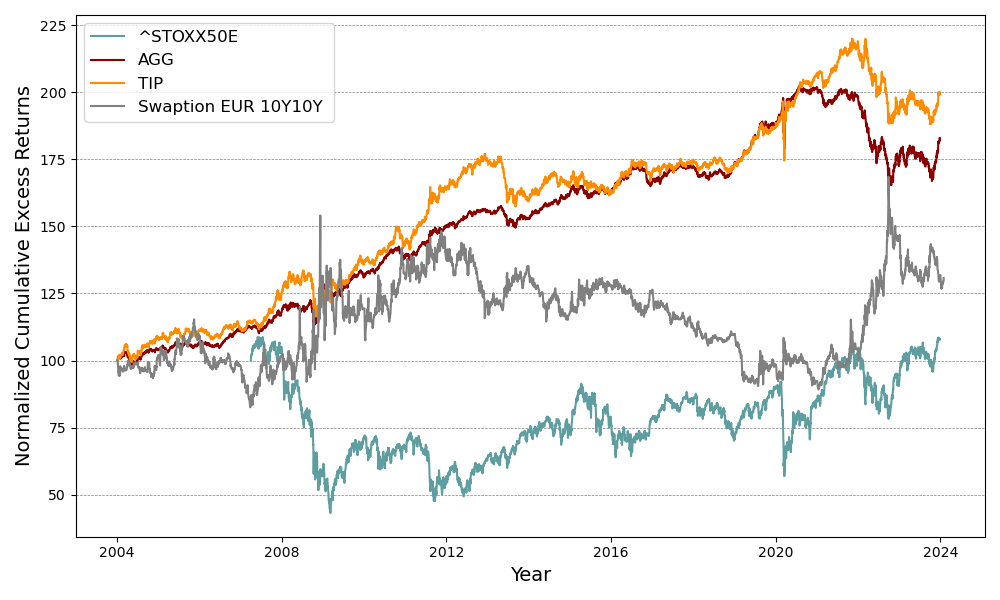
\includegraphics[scale = 0.4]{/Users/nannaingemannohrt/Desktop/master_thesis/main/plots/2004_to_2024_plot.png}
    \caption{Comparison of Normalized Cumulative Excess Return. Data source Citi Velocity 21.02.2024 
    and Yahoo Finance.}
    \label{fig:2004_2024}
\end{figure}
\noindent
Moving forward we will look at market data from Yahoo Finance and Citi Velocity. 
The purpose is to see how different asset classes perform under some particular markets situations.
First an introduction to the different tickers we will use to illustrate the different asset classes. 
We will like to compare perform of the asset classes equities, nominal bonds and inflation-linked bonds. 
The performance for the three asset classes will be compared to a swaption with ten years to expiry and a tenor
of ten years in euro, later in Chapter \ref{data_lab} the lingo of swaption will be covered. 
Below the chosen ticker are listed, with a short explanation. Where the ticker STOXX50E represent equities, 
AGG represent nominal bond and TIP illustrates inflation-linked bonds.

\begin{itemize}
    \item \textbf{STOXX50E} \text{---}  index of the 50 largest European equities.
    \item \textbf{AGG} \text{---}  index for US investment-grade bond. 
    \item \textbf{TIP} \text{---}  index for inflation-protected US-Treasury secitities.
    \end{itemize}
\noindent
Above in \autoref{fig:2004_2024} the three chosen ticker and the swaption development
is illustrated from 2004 to the start of 2024.
First of all we note that the same fluctuations appears across the three tickers. 
Secondly we note that these fluctuations does not appear in swaptions. 
We might even be able to see that the opposite fluctuation is present. 
Then lets remind yourself of some of the most important financial events during 
the time period from 2004 to 2024. First but not unnoticed we have the Global Financial Crisis
from 2007 to 2009.  Then we have the COVID-19 Pandemic in 2020 and most recently we have a 
longer period with high inflation starting i 2022. 
\\\\
To underline how swaption perform in these scenarios, we look a the specific time period
around some of the described events. Below in \autoref{fig:2007_2011} the same data is illustrated
from 2007 to 2011, this time period includes the Global Financial Crisis 2007 to 2009. 
From this time period we see that equities take a large jump down, where the development of the 
swaption was increasing. So during one of the worst drawdown period in the global market, 
swaptions kept performing. In \autoref{fig:2022_2024} we see the data displayed at the 
time period from 2022 to 2024, which is a period with high inflation. 
Here we clearly see that the swaption out perform the other asset classes. 
\\\\
This review on market data, underlines that swaption can add something different than some 
of the other asset classes. Therefore swaptions could add value to the portfolio constructions by adding diversification. 
But if swaptions should take part in the asset allocation, it is important to understand the instrument.
To understand swaptions as an instrument, we have to understand all the things contributing to the price
of a swaption. Then being able to price swaptions and analyzing them and managing the risk related to 
swaptions.  So moving forward we will start with a introduction to the mathematics of pricing swaptions. 
And troughout the thesis we will continue to develop knowledge of swaptions and the risk related to swaptions.
\begin{figure}[H]
    \centering
    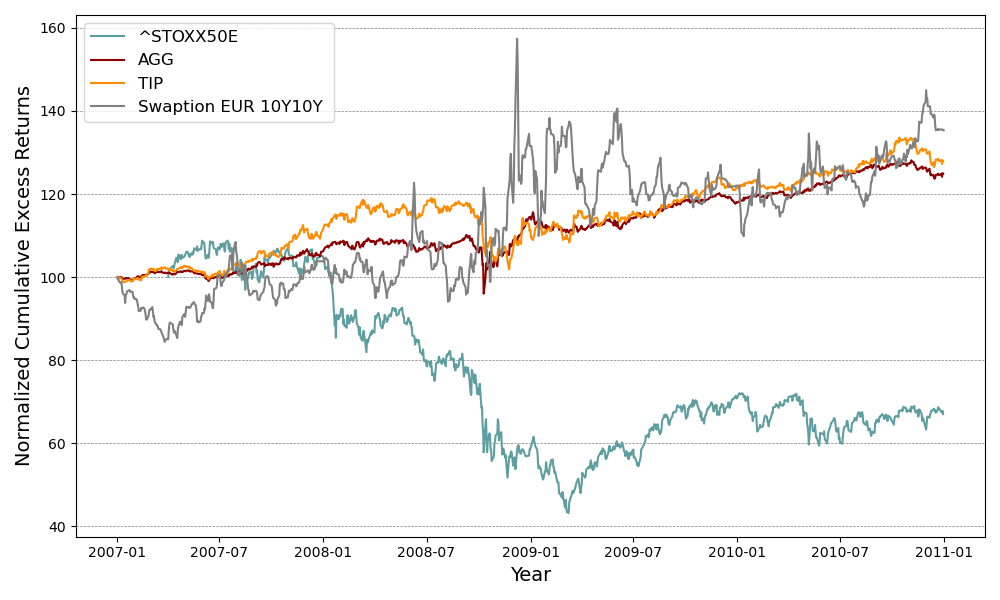
\includegraphics[scale = 0.4]{/Users/nannaingemannohrt/Desktop/master_thesis/main/plots/2007_to_2011.png}
    \caption{Global Financial Crisis 2007 to 2009.  Comparison of Normalized Cumulative Excess Return. Data source Citi Velocity 21.02.2024 
    and Yahoo Finance.}
    \label{fig:2007_2011}
\end{figure}
\noindent

\begin{figure}[H]
    \centering
    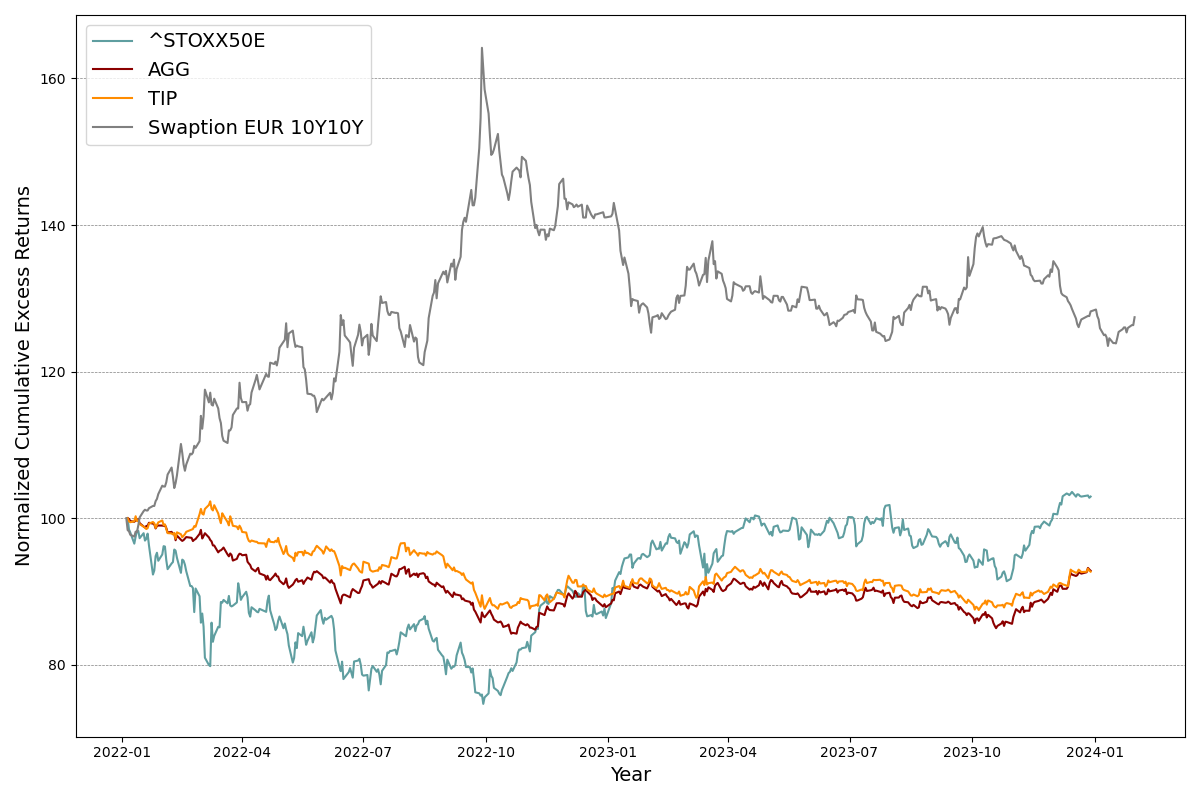
\includegraphics[scale = 0.4]{/Users/nannaingemannohrt/Desktop/master_thesis/main/plots/2022_to_2024.png}
    \caption{High inflation period 2022 to 2024. Comparison of Normalized Cumulative Excess Return. Data source Citi Velocity 21.02.2024 
    and Yahoo Finance.}
    \label{fig:2022_2024}
\end{figure}
\noindent


\newpage
\section{Mathematics of Pricing Swaptions}
To determine a swaption price it is important to understand what affects the price of the swaption. 
This Chapter simplifies this concepts by explaining interest rates, bonds, swaps-and options, 
and then shows how they come together to determine the price of a swaption.
\subsection{Time Value of Money}
Understanding the concept of interest rates begins with the fundamental idea that a dollar today holds 
more value than the same dollar in the future. To understand this concept, a discount factor is introduced as 
\begin{align*}
    B(t,T) = \text{value at time t of a dollar received at time T}
\end{align*} 
$B(t,T)$ refer to a contract that pays one dollar at maturity, T, which can be illustrated as below
\begin{align*}
    t & < T \rightarrow B(t,T) < 1 \\
    t & = T \rightarrow B(t,T) = 1
\end{align*}
The concept "Time Value of Money" asserts that the value of a dollar today is worth more than
the same amount in the future due to it's potential earning capacity and inflation.
The "Time Value Of Money" concept underpins various financial decisions, such as investing, borrowing,
and pricing financial instruments. Essentially, it recognizes that a dollar received today can be invested 
and earn interest over time, thereby increasing it's value. Conversely, a dollar received in the future
is subject to uncertainty and may not retain it's purchasing power due to inflation or other factors.
The discount factor represents the present value of future cash flows, taking into account the time value of money.
It reflects the idea that receiving a certain amount of money in the future is less valuable than receiving 
the same amount today.
\subsection{Zero Coupon Bonds}
One of the most common applications of the concept "Time Value Of Money" is zero coupon bonds. 
By construction, the mechanism of "Time Value Of Money" is present. This instrument 
have the common property of providing the owner with a deterministic (future) cash flow. 
\begin{definition}\label{def:zcb}
    A zero coupon bond with maturity date T, also called a T-bond, is a contract which 
    guarantees the holder one dollar to be paid at date T. The price at date t of 
    a bond with maturity date T is denoted by p$(t,T)$. \cite{Bjork} 
\end{definition} 
\noindent
Before moving forward we will look at the cashflow for a zero coupon bond. The illustration below shows that a time t,
the principal payment is made at the price $P(t,T)$ and at maturity T the principal is repaid.
\begin{center}
    \begin{tikzpicture}[font=\small] 
        \draw[-latex] (5,0) -- (13,0) node[anchor=north] {Time};
        \draw (6,0.2) -- (6,-0.5) node[above] at (6.,0.3)  {t};
        \draw (11.5,-0.2) -- (11.5,0.5) node[below] at (11.5,-0.3) {T};
        \draw (11.75,1.5) rectangle (11.25,0.5);
        \draw (5.75,-1.5) rectangle (6.25,-0.5) node[below, pos=.01] {Principal Payment};
        \node at (11.5, 2.0) {Principal Repayment };
    \end{tikzpicture}\\[10pt] 
    Illustration 3.1: Cashflow for a zero coupon bond
\end{center}

\subsection{The Yield Curve}
Where the concept "Time Value Of Money" and the discount factor are fundamental concepts used to assess the present value of future
cash flows, the yield curve provides insights into market expectations regarding future interest rates.
Understanding the interplay between these concepts is crucial for making informed investment decisions and pricing
financial instruments. The yield curve is a graphical representation illustrating the interest rates (bond yields) for various maturities.
Yield curves provides information about future interest rates and gives insight in the bond market today. 
The general intuition is that longer-term rates is higher than short-term rates, which in other words means that a
larger premium is expected for lending money over a longer period of time. This case sketches a yield curve with a 
positive slope, which is illustrated below.

\begin{center}
    \begin{tikzpicture} [scale=0.8]
        \begin{axis}[
            xlabel=Maturity,
            ylabel=Yield,
            no marks,
            axis lines=left,
            enlargelimits=false,
            clip=false,
            ymin=0,
            xmin=0,
            every axis y label/.style={
                at={(ticklabel* cs:1.05)},
                anchor=south,
             },
            every axis x label/.style={
                at={(ticklabel* cs:1.05)},
                anchor=west,
             },
            ]
            \addplot[domain=0:10, samples=100, thick] {x^(0.5)};
        \end{axis}
    \end{tikzpicture}\\[10pt] 
    Illustration 3.2: Yield curve with a positive slope
\end{center}
\subsection{Interest Rates}
\subsubsection{Spot Rates}
The spot rate represents the yield-to-maturity of a zero coupon bond,
while the forward rate refers to the anticipated interest rate in the 
future. The definition for determined spot rates as follows 
below
\begin{definition}\label{def:spot}
    The simple spot rate for $t<S<T$, henceforth referred to as the 
    LIBOR spot rate, is defined as \cite{Bjork} 
    \begin{align*}
        L(t;S,T) = - \frac{p(t,T)-p(t,S)}{(T-S)p(t,T)}
    \end{align*}
\end{definition} 
\noindent
\\\\
where $p(t,T)$ and $p(t,S)$ represent the price at time t of zero coupon bonds, that pay
1 dollar at time T and S, respectively. Intuitively, the spot rate $L(t;S,T)$ is the 
average rate of interest for borrowing or lending money over the time period from S to T, 
where such borrowing or lending is made at time t. 
\subsubsection{Forward rates}
Forward rates play a crucial role in financial markets, particularly in the realm of interest rate analysis and 
derivative pricing. They represent the interest rate applicable to a future period, agreed upon today.
Understanding forward rates requires grasping the concept of forward contracts and the expectations theory of interest rates.
Forward rates can be derived from the yield curve. The yield curve plots the yields of bonds with different maturities.
By analyzing the yield curve, one can infer the implied forward rates for future periods. For example, 
the forward rate between year 1 and year 2 is the rate at which an investor can borrow or lend money for the period
between year 1 and year 2, starting at year 1.
\\\\
Lets consider three time points on the yield curve $t=0,1,2$, where it is assumed
that $t_0 < t_1 < t_2$. At time $t_0$ we have the spot rates $p(t_0,t_1)$ and $p(t_1,t_2)$,
which represent the yields for bonds maturing at time $t_1$ and $t_2$ respectively.
Hence the forward rate, $R(t_1,t_2)$, can be determined using the equation below \cite{Bjork}
\begin{align*}
    R(t_1,t_2)= \frac{(1+p(t_0,t_2))^2}{(1+p(t_0,t_1))}-1
\end{align*}
Imagine investing one dollar in a one-year zero coupon bond, $B(t_0,t_1)$,
and instantly reinvesting the money received at time $t_1$ in a new one-year zero coupon bond,
$B(t_1,t_2)$, at a rate $R(t_1,t_2)$. This strategy should yield the same return as investing 
one dollar in a two-year zero coupon bond $B(t_0,t_2)$ and holding it for two years. 
This strategy illustrated the idea of forward rates. Let us then look a the general
formula for forward rates. 
\begin{definition}\label{def:forward}
    The continuously compounded forward rate for $[S,T]$ contracted at t is defined
    as \cite{Bjork} 
    \begin{align*}
        R(t;S,T)= - \frac{\log p(t,T)- \log p(t,S)}{(T-S)} 
    \end{align*}
\end{definition} 
\noindent
\\\\
So now formulas for spot rate and forward rates has been determined. To illustrate the differences between 
the two types of rates, a simple illustration below shows at which times the rates are determined. From the illustration
we see that all the spot rates are determine at time $t=0$, to each time point to maturity. Where the forward rates starts
a different time points. 
\\
\begin{center}
    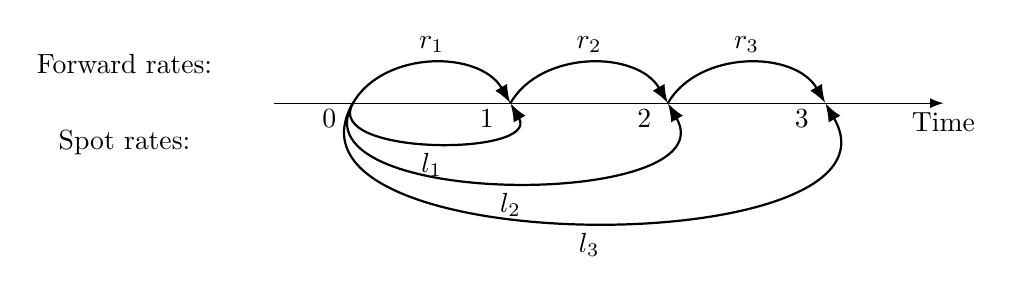
\begin{tikzpicture}
        \draw[-Latex] (2,0) -- (10.5,0) node[anchor=north] {Time};
        \draw[thick, -Latex] (3,0) to [out=60,in=120] node[above] {$r_1$} (5,0);
        \draw[thick, -Latex] (5,0) to [out=60,in=120] node[above] {$r_2$} (7,0);
        \draw[thick, -Latex] (7,0) to [out=60,in=120] node[above] {$r_3$} (9,0);
        \draw[thick, -Latex] (3,0) to [out=-120,in=-60] node[below] {$l_1$} (5,0);
        \draw[thick, -Latex] (3,0) to [out=-120,in=-60] node[below] {$l_2$} (7,0);
        \draw[thick, -Latex] (3,0) to [out=-120,in=-60] node[below] {$l_3$} (9,0);
        \node at (2.7, -0.2) {0};
        \node at (4.7, -0.2) {1};
        \node at (6.7, -0.2) {2};
        \node at (8.7, -0.2) {3};
        \node at (0.1,0.5) {Forward rates:};
        \node at (0.1,-0.5) {Spot rates:};
    \end{tikzpicture}\\[10pt] 
    Illustration 3.3: Forward and spot rates
\end{center}
\newpage
\subsection{Financial Derivatives}
\subsubsection{Bonds}
A bond is a debt security, like a loan. Borrowers issue bonds to raise money 
from investors willing to lend them money for a certain amount of time.
When you purchase a bond you are lending money to the issuer, which in 
some cases is a government or company. In return, from the construction of the 
bond, the issuer guarantees to pay a predetermined rate during the term of the bond
and repay the principal at maturity. 
\\\\
Earlier a zero coupon bond was introduced, and when talking about bonds, a zero coupon 
bond is the simplest representation of a bond. The zero coupon bond contract is 
only given by two cash flows. One for the buyer, that pays the issuer at time 
t = $t_0$, and another where the buyer receives the principal at time t = T.
Unlike other types of bonds, a zero coupon bond does not offer periodic 
interest payments (coupons) throughout its term. \cite{Bjork} 
\\\\
The price of a zero coupon bond is represented as 
p(t,T), where an individual lends an amount, K, with the intention of earning a
return in the future. Therefore, the price of a zero coupon bond, with 
its principal (also known as face value) K, at time t and with maturity 
T, is denoted as.
\begin{align*}
    p(t,T)= B(t,T)\cdot K
\end{align*}
\subsubsection{Fixed Coupon Bonds}
As describe, a zero coupon bond does not involve coupons throughout the term of the bond. 
But moving forward we will introduce various bond with coupons that are either fixed 
or floating. First we will consider the simplest form of a coupon bond, which is a 
fixed coupon bond. Fixed coupon bonds are a type of debt security that offers investors a predictable
return in the form of regular interest payments, known as coupons, until the bond's maturies.
These coupons are set at a fixed rate at the time of issuance, based on the bond's face value,
and are typically paid annually or semi-annually. Upon reaching maturity, the issuer repays 
the principal amount (face value) to the issuer, concluding the bond contract. The purpose
of a fixed coupon bond is the ability to provide a steady stream of income,
making them an attractive option for conservative investors seeking to minimize risk and 
secure predictable returns.
\\\\
Continuing, we will compute the price of a fixed coupon bond. First we note that the fixed coupon bond,
can be replicated by holding a portfolio consisting of zero coupon bond with maturities $T_i$, for 
$i=1,...,n$. So we will hold $c_i$ zero coupon bonds of maturities $T_i$ for $i=1,...,n-1$, and 
$K+c_n$ bonds with maturity $T_n$. Hence we have that the price, p(t), at time t, where $t<T$, of 
the fixed coupon bonds becomes. \cite{Bjork}
\begin{align*}
    p(t) = K \cdot p(t,T_n) + \sum_{i=1}^{n}c_i \cdot p(t,T_i)
\end{align*}
When talking about coupons, they are typically determined in terms of return rather than in monetary terms.
So the return of the i'th coupon is denoted as a simple rate, acting on the face value K, over the
time period $[t_{i-1},T_i]$. So for the i'th coupon the return is equal to $r_i$, and the face value 
is K, hence we have that 
\begin{align*}
    c_i = r_i(T_i-T_{i-1})K
\end{align*}
Where for standardized coupons, the time intervals will be equally spaced, which means that 
\begin{align*}
    T_i = T_0 + i \delta
\end{align*}
This also means the the coupon rates $r_1,...,r_n$ will be equal to a common coupon rate r. 
Hence the price p(t,T) of a fixed coupon bond where $t \leq T_1$ will be determined as below \cite{Bjork}
\begin{align*}
    p(t)= K \Big( p(t,T_n)+ r \delta \sum_{i=1}^{n}\cdot p(t,T_i) \Big)
\end{align*}
To end this section a illustration of the cashflow for a fixed coupon bond is illustrated below. 
\\
\begin{center}
    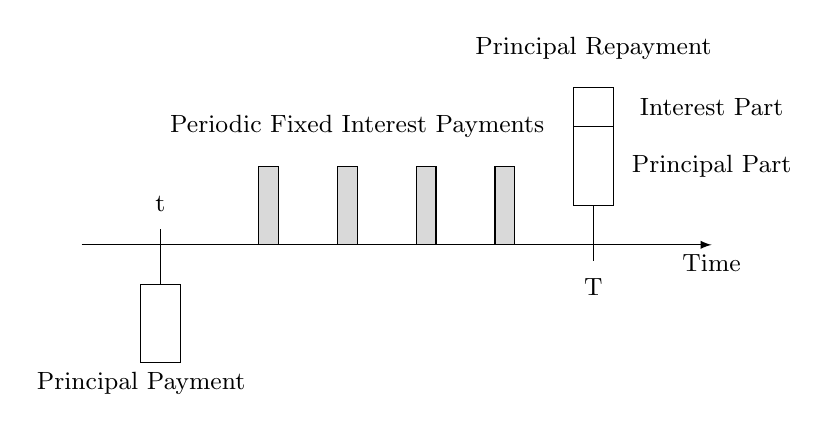
\begin{tikzpicture}[font=\small] 
        \draw[-latex] (5,0) -- (13,0) node[anchor=north] {Time};
        \draw (6,0.2) -- (6,-0.5) node[above] at (6.,0.3)  {t};
        \draw (11.5,-0.2) -- (11.5,0.5) node[below] at (11.5,-0.3) {T};
        \draw (11.75,1.5) rectangle (11.25,0.5) ;
        \draw (11.75,2) rectangle (11.25,1.5);
        \draw (5.75,-1.5) rectangle (6.25,-0.5) node[below, pos=.01] {Principal Payment};
        \draw[fill=black!15]  (10.5,0) rectangle (10.25,1);
        \draw[fill=black!15]  (8.5,0) rectangle (8.25,1);
        \draw[fill=black!15]  (9.5,0) rectangle (9.25,1);
        \draw[fill=black!15]  (7.5,0) rectangle (7.25,1);
        \node at (11.5, 2.5) {Principal Repayment};
        \node at (13.,1) {Principal Part};
        \node at (13.,1.75) {Interest Part};
        \node at (8.5, 1.5) {Periodic Fixed Interest Payments};
    \end{tikzpicture}\\[10pt] 
    Illustration 3.4: Cashflow for a fixed coupon bond
\end{center}
\subsubsection{Floating Rate Bonds}
Now a short introduction to fixed coupon bonds has been given, as mentioned there are also many 
other types of bonds that have floating coupons. When it is listed that there are bonds that have
floating coupons, what there is really said is that the rate is floating. So with the fixed coupon
bond, the coupon was predetermined when the agreement was made. But there are also bonds, where
the coupon is reset for every coupon period. These types of bonds is referred to as floating 
rate bonds. The most simple floating rate bond, is where the coupon rate $r_i$ is set to 
the spot LIBOR rate $L(T_{i-1}, T_i)$. Thus we have that 
\begin{align*}
    c_i = (T_i-T_{i-1})L(T_{i-1},T_i)K \quad \text{for} \quad i=1,...,n
\end{align*}
Here we have that $L(T_{i-1},T_i)$ is determined at time $T_{i-1}$, but the coupon is first 
delivered at time $T_i$. \cite{Bjork}  
\\\\
The LIBOR rate stands for London InterBank Offered Rate, which is a rate the the 
British Bankers Association sets every business day. Like the LIBOR rate, there is many types
of xIBOR rates, one is EURIBOR rate which is a rate the 
European Banking Federation sets every business day. 
\\\\
These different type of xIBOR rates are sets differently, but they all use the money market convention. 
So when taking about business day, the money market convention is important. This is a day-count 
convention is a standardized methodology for calculating the number of days between two dates.
This means that when $t <T_0$  the coupon dates are equally spaced with  
\begin{align*}
    \delta = T_{i}-T_{i-1}
\end{align*}
To determined the value of a the simplest floating rate bond, the LIBOR spot rate we can without
loss of generality assume that K=1 and insert Definition \ref{def:spot} of the LIBOR spot rate 
to obtain
\begin{align*}
    c_i &= (T_i-T_{i-1})L(T_{i-1},T_i)K \\
        &= \delta L(T_{i-1},T_i) \\
        &= \frac{1- p(T_{i-1},T_i)}{\delta p(T_{i-1},T_i)} = \frac{1}{p(T_{i-1},T_i)}-1
\end{align*}
Then we have found the price of the LIBOR spot rate, where $\frac{1}{p(T_{i-1},T_i)}$ is zero coupon bonds price. 
So the next step is to determine the price for the floating rate bond. If we look at the $T_i$-payment of the floating rate bond, 
it has the value of
\begin{align*}
    P(t,T_{i-1})-P(t,T_i)
\end{align*}
If we then sum over all the i payments of the floating rate we obtain that the floating rate bond value is
\begin{align*}
    p(t)= p(t,T_n) + \sum_{i=1}^{n}\Big[p(t,T_{i-1})-p(t,T_i)\Big] = p(t,T_0) 
\end{align*}
where we note that if $t=T_0$ we get that $p(T_0)=1$ \cite{Bjork}. \\\\
Like for the section for the fixed coupon bond, a illustration of the cashflow for a floating rate bond is illustrated below.
From the to illustrations we clearly see the different in the periodic interest payments. 
\begin{center}
    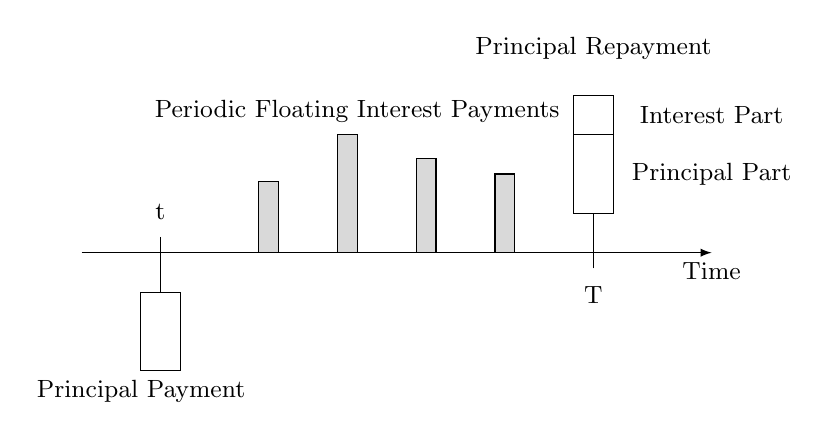
\begin{tikzpicture}[font=\small] 
        \draw[-latex] (5,0) -- (13,0) node[anchor=north] {Time};
        \draw (6,0.2) -- (6,-0.5) node[above] at (6.,0.3)  {t};
        \draw (11.5,-0.2) -- (11.5,0.5) node[below] at (11.5,-0.3) {T};
        \draw (11.75,1.5) rectangle (11.25,0.5) ;
        \draw (11.75,2) rectangle (11.25,1.5);
        \draw (5.75,-1.5) rectangle (6.25,-0.5) node[below, pos=.01] {Principal Payment};
        \draw[fill=black!15] (10.5,0) rectangle (10.25,1);
        \draw[fill=black!15]  (8.5,0) rectangle (8.25,1.5);
        \draw[fill=black!15]  (9.5,0) rectangle (9.25,1.2);
        \draw[fill=black!15] (7.5,0) rectangle (7.25,0.9);
        \node at (11.5, 2.6) {Principal Repayment};
        \node at (13.,1) {Principal Part};
        \node at (13.,1.75) {Interest Part};
        \node at (8.5, 1.8) {Periodic Floating Interest Payments};
    \end{tikzpicture}\\[10pt] 
    Illustration 3.5: Cashflow for a floating rate bond
\end{center}
\newpage
\subsection{Interest Rate Swaps}
Now some simple cases of different types of bonds has be introduced. Then we will combine the knowledge we have gained to move on
to take interest rate derivatives into consideration. Again we will consider the simplest type of a interest rate derivative, which is a
interest rate swap. The construction of a interest rate swap is that there is an  exchange of a payment stream of a fixed rate of interest,
which is know as the swap rate. This fixed rate is exchanged for some floating rate, such as the LIBOR rate. 
As mentioned the fixed rate is know as the swap rate, this swap rate is determined from forward rate extracted from the yield curve, 
so it makes the present value of the swap equal to zero. This we will formulate formally later. 
\\\\
As stated in the interest rate swap, two cash flow are exchanged, where one of is a 
fixed cash flow and the other is a floating cash flow. These components of
the interest rate swap are known as the "fixed leg" and the "floating leg". 
The role of each participant in the swap is determined in relation to the 
fixed leg: the party making fixed payments is engaged in a "payer swap," 
while the party making floating payments (and receiving fixed payments) is
involved in a "receiver swap.". The two involved cashflow there are exchanged form the "receiver" to the "payer" is illustrated below.
\\
\begin{center}
    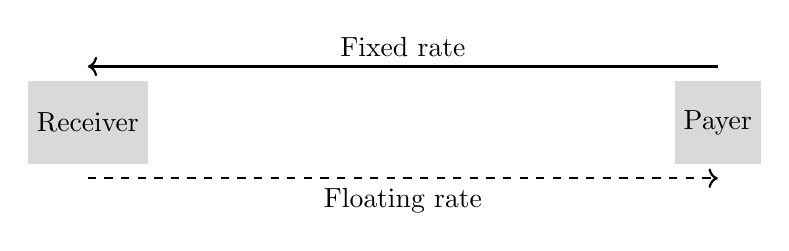
\begin{tikzpicture}
        \tikzstyle{receiver} = [rectangle, fill=black!15, text centered, minimum height=3em]
        \tikzstyle{payer} = [rectangle,  fill=black!15, text centered, minimum height=3em]
        \node[receiver] (receiver) {Receiver};
        \node[payer, right of=receiver, node distance=8cm] (payer) {Payer};
        \draw[thick, <-] ([yshift=5pt]receiver.north) -- node[above] {Fixed rate} ([yshift=5pt]payer.north);
        \draw[thick, dashed, ->] ([yshift=-5pt]receiver.south) -- node[below] {Floating rate} ([yshift=-5pt]payer.south);
    \end{tikzpicture}\\[10pt] 
    Illustration 3.6: Cashflow for fixed and floating rate exchanges
\end{center} 
\noindent
Again we have that K is the principal also know as the face value and we will denote the swap rate, R.
Further we have that payments
arises at the dates $T_1,...,T_n$, this means that at time $T_i$ the buyer of the interest rate swap will pay
\begin{align}
    K \delta L(T_{i-1},T_i)
    \label{irs}
\end{align}
where we have that $L(T_{i-1},T_i)$ is the spot rate, which could be the LIBOR spot rate.
It is also assumed
that the days $T_0,...,T_n$ is equally spaced with $\delta = T_i - T_{i-1}$ as mentioned above in the section for floating rate bonds. 
Then it is noticed that the expression in \autoref{irs} is the same as $Kc_i$, where again $c_i$ is the i'th coupon for the floating rate. 
So at time $T_i$ the buyer will pay $K \delta R$, where the cash flow at time $T_i$ is given by below
\begin{align*}
    K \delta \Big[L(T_{i-1},T_i)-R \Big]
\end{align*}
Then by applying the results from the section for floating rate bonds again, we are able to compute the value of the 
cash flow at time $t<T_0$. The value of the cash flow is listed below
\begin{align*}
    K p(t,T_{i-1})-K(1+\delta R)p(t,T_i)
\end{align*}
Hence we have that the total value denote by $\Pi(t)$, so the total value at time t of the swap is given as below
\begin{align}
    \pi (t) = K \sum_{i=1}^{n} \Big[p(t,T_{i-1})-(1+ \delta R)p(t,T_i)\Big]
    \label{valueirs}
\end{align}
Moving forward we simplify \autoref{valueirs} in the below Proposition \ref{simple} \cite{Bjork}.
\\
\begin{proposition}
    The price, for $t<T_0$, of the swap in \autoref{valueirs} above
    is given by 
    \begin{align*}
        \Pi(t) = K p(t,T_0)-K \sum_{i=1}^{n}d_i p(t,T_i)
    \end{align*}
    where
    \begin{align*}
        d_i &= R \delta, \quad i=1,...,n-1 \\
        d_n &= 1+ R \delta
    \end{align*}
    \label{simple}
\end{proposition}
\noindent 
To sum up on interest rate swaps, let consider a timeline for a payer swap contract. Where the issuer is paying the fixed leg 
and receiving the floating leg. The timeline of the contract is illustrated below, where a time t the contract is made. 
Then the swap start a time $T_S$ and maturities at time $T_E$.
The squiggly lines denote the floating interest payments that the payer will make based on the interest rate observed 
at the beginning of the period and the end of the period. The vertical lines at the beginning of each period represent
the fixed payment dates, and the horizontal dotted line indicates the continuation of the swap contract over time.
\begin{center}
    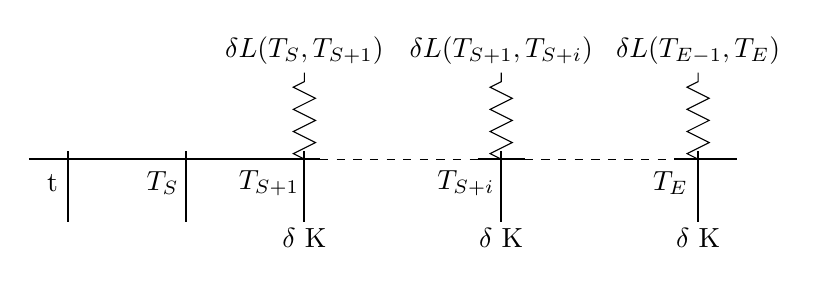
\begin{tikzpicture}
        \draw[thick] (0,0) -- (3.7,0);
        \draw[dashed](3.7,0) -- (5.7,0);
        \draw[thick] (5.7,0) -- (6.3,0);
        \draw[dashed](6.3,0) -- (8.2,0);
        \draw[thick] (8.2,0) -- (9.0,0);
        \draw[thick] (0.5,0.1) -- (0.5,-0.8) node at (0.3,-0.3) {t} ;
        \draw[thick] (2,0.1) -- (2,-0.8) node at (1.7,-0.3) {$T_S$} ;
        \draw[thick] (3.5,0.1) -- (3.5,-0.8) node at (3.05,-0.3) {$T_{S+1}$} ;
        \draw[thick] (6.0,0.1) -- (6.0,-0.8) node at (5.55,-0.3) {$T_{S+i}$} ;
        \draw[thick] (8.5,0.1) -- (8.5,-0.8) node at (8.15,-0.3) {$T_{E}$} ;
        \draw[decorate, decoration={zigzag, segment length=8pt, amplitude=4pt}] (3.5,0) -- node[above=15pt] {$\delta L(T_{S}, T_{S+1})$} (3.5,1.1);
        \draw[decorate, decoration={zigzag, segment length=8pt, amplitude=4pt}] (6,0) -- node[above=15pt] {$\delta L(T_{S+1}, T_{S+i})$} (6,1.1);
        \draw[decorate, decoration={zigzag, segment length=8pt, amplitude=4pt}] (8.5,0) -- node[above=15pt] {$\delta L(T_{E-1}, T_{E})$} (8.5,1.1);
        \node at (3.5,-1.) {$\delta$ K};
        \node at (6,-1.) {$\delta$ K};
        \node at (8.5,-1.) {$\delta$ K};
    \end{tikzpicture}\\[10pt] 
    Illustration 3.7: Cashflow for a payer swap 
\end{center}
Earlier we left behind a discussion of how the swap rate, R,  is determined. 
It was noted that the swap is determined such that the present value of
the swap is equal to zero. Now we will give a more accurate definition of how swap rates is determined in Proposition \ref{swaprate1}.
\begin{proposition}
    If, by convention, we assume that the the contract is written at $t=0$, 
    the swap rate is given by \cite{Bjork}
    \begin{align*}
        R = \frac{p(0,T_0)-p(0,T_n)}{\delta \sum_{i=1}^{n}p(t,T_i)}
    \end{align*} 
    \label{swaprate1}
\end{proposition}
\noindent 
If we have that $T_0=0$ the formula for the swap rate, R, becomes
\begin{align*}
    R= \frac{1-p(0,T_n)}{\delta \sum_{1}^{n}p(0,T_i)}
\end{align*}
\newpage
\subsection{Options}
In this section will introduce the framework of options in the over-the-counter-market. 
The purpose of this section is to establish a pricing formula for European call options.
The meaning of introducing pricing of options before introducing swaptions pricing, is that a swaption is  a 
more complex derivative. So the idea is to get a fundamental understanding of pricing derivatives in a more simple case.
\\\\
Firstly, let's clarify what the over-the-counter market (OTC) is. It is  a marketplace where numerous trades occur.
In the OTC market private companies exchange trades, these companies are firms as banks, other 
large financial institutions and funds managers \cite{Hull}. Then we have established the market where 
options is traded, so moving forward we will look in to options contracts. 
\\\\
A call options gives the holder the right to buy the underlying asset at a fixed strike price, K, at a 
predetermined time, T. Where a put option gives the holder the right to sell the underlying asset at a fixed
strike price, K, and a predetermined time, T. Options contracts come in various types, with the 
most common being the European and American options, followed by Bermudan options. European options can only 
be exercised at the maturity date, while American options can be exercised at any time point upon to the maturity date.
Bermudan options allow exercise at specific predetermined time points.
For the purpose of understanding the basics of options pricing, we will focus on the European option. 
The contract functions, $\Phi$, for European call and put options are as follows.
\begin{align}
    \Phi(x)_{\text{call}} &=  \max[S-K,0] \label{call_function}\\ 
    \Phi(x)_{\text{put}} &= \max [K-S,0] \label{put_function}
\end{align}
where K is the strike price, S denotes the market price of the underlying asset \cite{Bjork}. From \autoref{call_function} and \autoref{put_function} we see
that the value of the contract function can not be negative, since in both cases the contract function is a 
function there takes the maximum of the payoff and zero. So the holder maximum lost is the paid premium. Below the described contract
function for a European call option is illustrated.
\begin{center}
    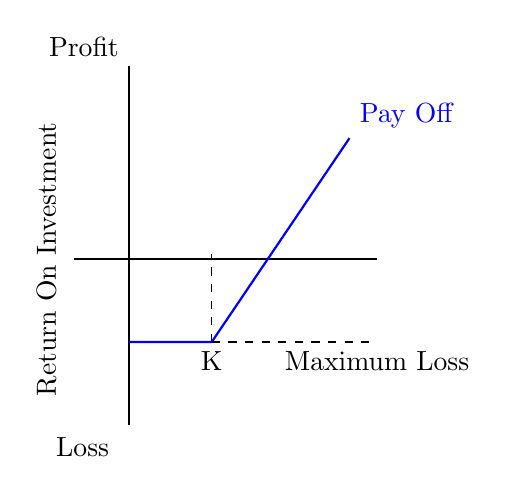
\begin{tikzpicture}[scale=0.7]
        \draw[thick] (-1,0) -- (4.5,0) ;
        \draw[thick] (0,-3) -- (0,3.5) node[anchor=south east] {Profit};
        \coordinate (K) at (1.5,-1.5);
        \draw[dashed] (K) node[below] {K} -- ++(0,1.6);
        \draw[thick, blue] (0,-1.5) -- (K) -- (4,2.2) node[anchor=south west] {Pay Off};
        \draw[dashed] (1.5,-1.5) -- (4.5,-1.5) node[below] {Maximum Loss};
        \draw (-1.5,-3.4) node[anchor=west] {Loss};
        \node[rotate=90] at (-1.5,0) {Return On Investment};
    \end{tikzpicture}\\[10pt] 
    Illustration 3.8: Contract function for a European call option
\end{center}
\subsubsection{Risk Neutral Measure} \label{risk_neutral_section}
Before options pricing a brief introduction to the risk neutral measure will be covered.
When options are priced the value of the options is calculated by discounting 
the options expected payoff at time T under the risk neutral measure $\QQ$. 
\\\\
The value of the options is calculated under the risk neutral measure $\QQ$ also know as the pricing measure, and 
not under the actual measure $\PP$. The $\PP$- measure reflects the real world probabilities. If prices was determined 
under $\PP$ is could lead to arbitrage opportunities, because it would reflect the actual risk preferences of
investors, who demand different rates of return for different risks. Under the risk neutral measure $\QQ$  
probabilities are shifted or adjusted in such way that the expected rate of return on assets becomes the risk free rate. 
This adjustment removes the risk premiums that are present in the actual probability measure $\PP$.
This lead to the First Fundamental Theorem of Asset Pricing, to develop this theorem we consider 
the concept of martingales. 
A stochastic process $X_t$ is a $\QQ$-martingale, if the process has no drift term (dt-term). Which is satisfied if it holds that
$\EE_{t}^{\QQ}\Big[X_T\Big] = X_t$ for all $t<T$. Next we will consider a price process $X_t$ with the following dynamic.
\begin{align}
    d X_t = r_t X_t dt + \sigma X_t d W_{t}^{\QQ}
    \label{price_process}
\end{align}
where $W_{t}^{\QQ}$ is $\QQ$-Wiener process and  $r_t$ is the process for the risk free interest rate. $r_t$ can be looked at the locally risk free rate return 
from a continuously compounded bank account $B(t)= \text{exp} \Big[\int_{0}^{t}r(s)ds \Big]$.
Where the bank account has the following dynamic
\begin{align}
    dB(t) &= r(t)B(t) dt \label{bank1}\\
    B(0) & = 1 \label{bank2}
\end{align}
If we look at \autoref{price_process} we see there is a dt-term present, so it is not a martingale.
But if we discount the price process, this will be a martingale do to the martingale property below
\begin{proposition}
    (\textbf{The Martingale Property}) In the Black-Scholes model, the price process $\Pi_t$
    for every traded asset, be it the underlying or derivative asset, has the property that the normalized price process
    \begin{align*}
        Z_t = \frac{\Pi_t}{B_T}
    \end{align*}
    is a martingale under the measure $\QQ$ \cite{Bjork}
\end{proposition}
\noindent 
This lead os to the First Fundamental Theorem of Asset Pricing in \autoref{frist_theorem_of_asset_pricing}.
\begin{theorem}
    (\textbf{First Fundamental Theorem of Asset Pricing})
    Given a time horizon, a risky asset with price process $X_t$ and a
    risk free asset with price process $B_t$, the market is arbitrage free 
    (under the probability measure $\PP$) if and only if there exists an 
    equivalent probability measure $\QQ$ such that the discounted price process
    $\Big[\frac{X_t}{B_t}\Big]$  is a $\QQ$- martingale \cite{Bjork}
    \label{frist_theorem_of_asset_pricing}
\end{theorem}
\noindent 
Hence we have establish the First Fundamental Theorem of Asset Pricing. So to sum up in order to be able to calculate
option prices, the "fair" or arbitrage free price, there must exist a risk neutral measure $\QQ$, such the the discount prices
is a $\QQ$-martingale. 
\subsubsection{Options Pricing}
The next question to be answered is what is the "fair" price of these options, we will denote the price of
the option by $\Pi(t)$. Again to simplify we will consider
the European call option moving forward. To determine the price of a European call potion, we wil use the 
Black-Scholes formula. This requires a review of Risk Neutral Valuation and the Black-Scholes model.
\\\\
Risk Neutral Valuation determine the value of an asset by discounting the expected values of the assets future 
pay-offs at the risk free rate of return, this formalized in \autoref{rnt} below.
\begin{theorem}
    \textbf{(Risk Neutral Valuation)} The arbitrage free price of the claim $\Phi(S_t)$ is given by \\
    $\Pi(t)[\Phi]$=$F(t,S_t)$, where F is given by the formula 
    \begin{align*}
        F(t,s) &= -e^{-r(T-t)} \EE_{t,s}^{\QQ} \Big[\Phi(S_T)\Big]
    \end{align*}
    where the Q-dynamics os S is
    \begin{align*}
        dS_t & = r S_t dt + S_t \sigma(t,S_t) dW^{\QQ} \\
        S_0 & = s
    \end{align*}
    and $W^{\QQ}$ is a $\QQ$-Wiener process \cite{Bjork}
    \label{rnt}
\end{theorem}
\noindent 
The Risk Neutral Valuation has been introduced, hence the only thing left before we are able to price a 
European call option, is to establish the model the price in found under. In this case it is the Black-Scholes model.
It consists of two asses, a risk free asset with price process, B, and a stock price with price process, S.
The dynamics of the two assets is listed below
\begin{align*}
    dBt & = rB_t dt \\
    dS_t &= \mu S_t dt + \sigma S_t dW_t
\end{align*}
where the short rate, r, is  a deterministic constant,  $\mu$ and $\sigma$ is two constants. It is also assumed
that the stock price process is lognormal distributed. From \autoref{rnt}
(Risk Neutral Valuation) the formulas for determine the arbitrage free price is available. Finally the requirements
for being able to price a European option is satisfied, hence we have the Black-Scholes Formula below.
\begin{proposition}
    \textbf{(Black-Scholes Formula)} The price of a European call option with strike K and time of maturity T 
    is given by the formula $\Pi$ = $F(t,S_t)$
    \begin{align*}
        F(t,S_t) & =s N[d_1(t,s)] -e^{-r(T-t)}KN[d_2(t,s)] 
    \end{align*}
    Here N is the cumulative distribution function for the N $[0,1]$ distribution and 
    \begin{align*}
        d_1(t,s) &= \frac{1}{\sigma \sqrt{T-t}} \Big[ \ln \Big(\frac{s}{K} \Big) +  \Big(r + \frac{1}{2} \sigma^2)(T-t)  \Big] \\
        d_2(t,s) &= d_1(t,s)-\sigma \sqrt{T-t}
    \end{align*}
    \label{Black-Scholes Formula}
    \cite{Bjork}
\end{proposition}
\subsection{Swaptions}
Now that we have establish a foundational understanding of interest rates, bonds, swaps and options, we can
now go deeper into swaptions. First we will explain what constitutes a swaption and the we will continuing 
to develop the framework of pricing a swaption, built on the knowledge we have established.  
\\\\
A swaption is a financial derivative that can be describeed as an option to exchange a fixed rate bond for
floating rate bonds for a predetermined principal. 
There are two types of swaptions, payer swaptions and receiver swaptions.
A payer swaption gives the holder the right to pay a fixed interest rate and receive a floating rate, 
similar to a call option in the stock market. On the other hand, a receiver swaption allows the holder
to pay a floating interest rate and receive a fixed rate, resembling a put option \cite{Lindstrom} .

\subsubsection{Swaption Pricing}
Swaptions pricing purpose is to calculating the present value of expected payments from the swap contract,
should the option be exercised. The pricing model must take various factor into account, such as the
volatility of interest rates, the term structure of interest rates, and the time value of money. 
To price swaptions, the Black model will be used, which is an extension of the Black Scholes
model for equity options. The choice of using the Black model for pricing swaption is commonly used, especially when
is purpose is the price European swaption. Likewise for swaps, there is also different type of swaptions. 
Again European options can only be exercised at the maturity date, while American options can be exercised
at any point in time up to the maturity date. Moving forward we will only consider European swaptions. 
The Black model assumes that the underlying swap rate follows a lognormal distribution and uses a 
risk neutral valuation approach. These concept has been reviewed earlier, hence we can the move on to 
formulating pricing swaptions.
\\\\
First we consider a swaption that is settled such that the holder has the right to pay a fixed rate, $S_K$, 
and receive a floating rate on the swap that will expire in n year starting in T years.
Further we will assume that there are m payments 
per year under the swaption and we will let the notional principal be denoted by L. These m payments has
assumed that each fixed payment on the swap is the fixed rate times L/m. Next we suppose that 
the given swap rate for an n-year swap staring a time T, is denoted by $S_T$. 
From the knowledge on swaps we formulate the payoff function of the swaption, which is listed in
\autoref{swaptionspay} below
\begin{align}
    \frac{L}{M} \max \Big( S_T - S_K, 0 \Big)
    \label{swaptionspay}
\end{align}
We note that the cashflow generated from the payoff function of the swaption, is reviewed m times 
a year. The most commonly frequency payments is semi-annually and annually. These payments at m times
of a year, is paid throughout the life of the swap. The payment of the swap, have the following 
payments dates 
\begin{align*}
    T_1,T_2,...,T_{mn}
\end{align*}
Let us be reminded that a swaption is a option on the swap rate, which is the one that generated the payoffs.
Then we formulated the price of the payer swaption as \cite{Hull}
\begin{align*}
    \Pi(t)_{\text{Payer swaption}} = \sum_{i=1}^{mn} \frac{L}{m} p(0,T_i)\Big[ S_F N(d_1) - S_K N(d_2)\Big] \quad \text{for} \quad T_i= T+i/m  
\end{align*}
where
\begin{align*}
    d_1 & = \frac{1}{\sigma \sqrt{T}} \Big[ \ln \Big(\frac{S_F}{S_k}\Big)+\sigma^2\Big(\frac{T}{2}\Big)\Big] \\
    d_2 & = d_1-\sigma \sqrt{T}
\end{align*}
Where N is the cumulative distribution for the $N [0,1]$ distribution, $S_F$ is the forward swap rate a time
zero, $\sigma$ is the volatility of the forward swap rate. The term $\sum_{i=1}^{mn} \frac{L}{m} p(0,T_i)$ 
is the discount factor for the mn payoffs. To simplify we define A as the values of the contract that
pays $1/m$ at times $T_i ( 1\leq i \leq mn)$ a in \autoref{a_simple}
\begin{align}
    A= \frac{1}{m} \sum_{i=1}^{mn} p(0,T_i)
    \label{a_simple}
\end{align}
Hence we have that the value of the swaption can be expressed as 
\begin{align*}
    L N \Big[S_F N(d_1) - S_K N(d_2) \Big]
\end{align*}
Which leads to the case we looked at, where the contract of the swaption was made such that the 
holder has the right to receive a fixed rate of $S_K$ instead of paying it. It also leads to
the payoff of the swaption as listed in \autoref{payoff_swaption} below. We note that the payoff 
is a payoff function of a put option on $S_T$. 
\begin{align}
    \frac{L}{M} \max \Big( S_K - S_T, 0 \Big)
    \label{payoff_swaption}
\end{align}
Finally we can end this section with the value of a swaption in a standard market model \cite{Hull}.
\begin{align*}
    \Pi(t)_{\text{swaption}}= L A \Big[S_K N(-d_2) - S_F N(-d_1)\Big]
\end{align*}
To summarize the mathematics of pricing a swaption has been reviewed, which include introducing interest rates, 
bonds, swaps and option. It is important to remember which choices was made along the way,
because the price of the swaption depends on the choice of the model. But now the simplest case has been 
introduced, so we can move forward with the analysis.  
\newpage
\section{One-Factor Short-Rate Model}
As we have established, interest rate is crucial 
for pricing swaptions. Therefore, this chapter will 
begin by examining the general one-factor short rate 
model. It will then continue with a closer look at the 
Vasicek model, where we will determine its properties. 
To support and investigate these properties, a small 
simulation analysis of the Vasicek model will be 
performed.
\\\\
The risk-free short rate, r, is sometimes referred to as the instantaneous short rate. 
The concept is used in finance modeling to represent the continuously compounded interest rate for 
short time intervals. The short rate, r, is often modeled using stochastic differential equations in 
mathematical finance. The typical models for modeling the short rate is the Vasicek model and the Cox–Ingersoll–Ross model, 
later the Vasicek model will be covered. When pricing derivatives as bonds and options, the price depends on 
the process followed by r in the risk-neutral world \cite{Hull}.
\\\\
As discussed in the Section \ref{risk_neutral_section} - Risk Neutral Measure, $r_t$, can be looked at the locally risk-free 
rate from a continuously compounded bank account $B(t)= \exp \Big[\int_{0}^{t} r(s) ds \Big]$. 
Where the bank account has the dynamic listed in \autoref{bank1} and \autoref{bank2}.
Postulation: the considered market is arbitrage-free, wich due to the First Fundamental Theorem of Asset Pricing, 
if stating that there exist a probability measure $\QQ$, equivalent to $\PP$, all asset prices discounted by $B(t)$
are $\QQ$-martingales. In other words under the considered market for any T we have that 
\begin{align}
    \frac{P(0,T)}{B(0)} = P(0,T) = \EE^{\QQ} \Big( \frac{P(T,T)}{B(T)}\Big) = \EE^{\QQ} \Big( \frac{1}{B(T)}\Big) 
    = \EE^{\QQ} \Big( \exp \Big[ - \int_{0}^{t}r(s)ds \Big] \Big)
    \label{dist}
\end{align}
where $P(0,T)$ is the price at time zero of the asset and note that $P(T,T)=1$. So \autoref{dist} says that 
the time zero price of the asset are $\QQ$-expectations  of the payoff \cite{Bermudan}.
In other words in a market free of arbitrage, bond prices are determined by the risk-neutral expectations 
of how the short-term interest rate will behave. Because all types of interest rate instruments are based
on bond prices, the entire term structure or zero coupon curve can be described by the distributional properties
of just one state variable - the short rate \cite{Bermudan}.

\subsection{The Vasicek Model}
So all interest rate instruments are fundamentally dependent on bond prices. Understanding the movements of 
these prices is essential for accurately describing the term structure or zero coupon curve. The behavior 
of the short rate, a key variable, underlies this understanding due to its distributional properties.
\\\\
The Vasicek model, introduced by Oldrich Vasicek in 1977, serves as a robust framework to analyze these dynamics.
The Vasicek model is renowned for its simplicity and the ease with which it facilitates bond price calculations, 
the model assumes that the short-term interest rate adheres to a mean-reverting stochastic process. This process is characterized 
by parameters that dictate the rate's mean reversion speed, its long-term average level, and its volatility.
The model is used for forecasting how interest rates in the market will develop in the future. The model is a
mathematical result of interest rates and it is a one-factor short rate model and the model is constructed in the 
term of that the evolution of interest rates only depends on one stochastic variable.
\\\\
So now a short introducing to the Vasicek model has been covered and the next step is to look closer at the 
mathematical framework of the Vasicek model. The Vasicek model consists of the dynamic of the short rate under the $\PP$-measure
(the real world measure). Where the dynamic of the short rate is governed by a stochastic differential equation. 
The dynamic for the short rate in the Vasicek model is presented below in \autoref{vas_dyn1} and \autoref{vas_dyn_r0} \cite{Bjork}.
\begin{align}
    d r_t &= \kappa \Big[\theta -r(t)\Big] dt + \sigma d W(t) \label{vas_dyn1}\\
    r(0) &= r_0 \label{vas_dyn_r0}
\end{align}
The dynamic for the short rate in \autoref{vas_dyn1} is a Ornstein-Uhlenbeck process, which is a type of stochastic 
differential equation that describes the evolution of a mean-reverting behavior. So the process is consisting of a 
tendency to revert towards the mean of the process. This tendency is illustrated in \autoref{fig:vasicek} below, where 
 rates is simulated using the Vasicek model for some chosen parameters listed in \autoref{tab:parameters_short_rate} below. 
 Note in \autoref{fig:vasicek}
one simulated path of the short rate is illustrated. Where in \autoref{fig:vasicek-sim} ten simulated paths are illustrated,
but the same tendency appears. The parameters in the short rate dynamic
$\kappa$, $\theta$ and $\sigma$ are positive constants. Where $\kappa$ represent the mean reversion speed, $\theta$ 
is the long-term average rate, $\sigma$ is the volatility  and $W(t)$ is a Wiener process \cite{Bermudan}. 
\\
\begin{table}[H]
    \centering
    \begin{tabular}{ccc}
      \toprule
      \textbf{Parameter} & \textbf{Parameter explanation} & \textbf{Value} \\
      \midrule
      \rowcolor{lightgray!40} $T$ & Time to maturity & 10 \\
      $r_0$ & Initial short rate & 0.05 \\
      \rowcolor{lightgray!40} $\kappa$ & Mean reversion speed & 0.2\\
      $\theta$ & Long-term average rate  & 0.03 \\
      \rowcolor{lightgray!40}$\sigma$ & Volatility& 0.02 \\
      \bottomrule
    \end{tabular}
    \caption{Summary of parameters used for simulation the short rate in the Vasicek model}
    \label{tab:parameters_short_rate}
\end{table}
\noindent
\begin{figure}[H]
    \centering
    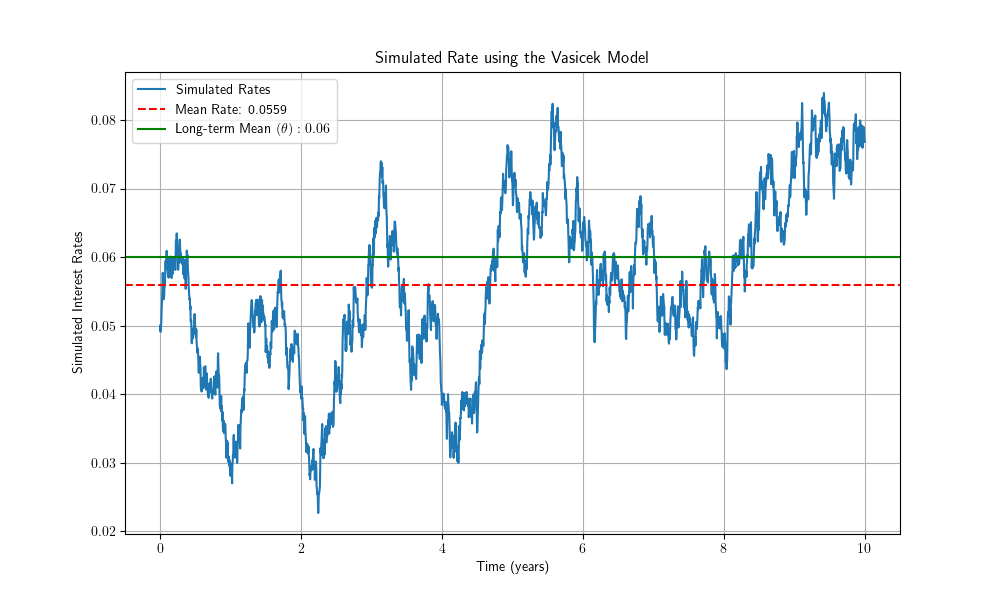
\includegraphics[width=0.75\linewidth]{/Users/nannaingemannohrt/Desktop/master_thesis/main/plots/VasicekModelPlot.png}
    \caption{Plot of one simulated rate path  using the Vasicek model.}
    \label{fig:vasicek}
\end{figure}
\noindent
\begin{figure}[H]
    \centering
    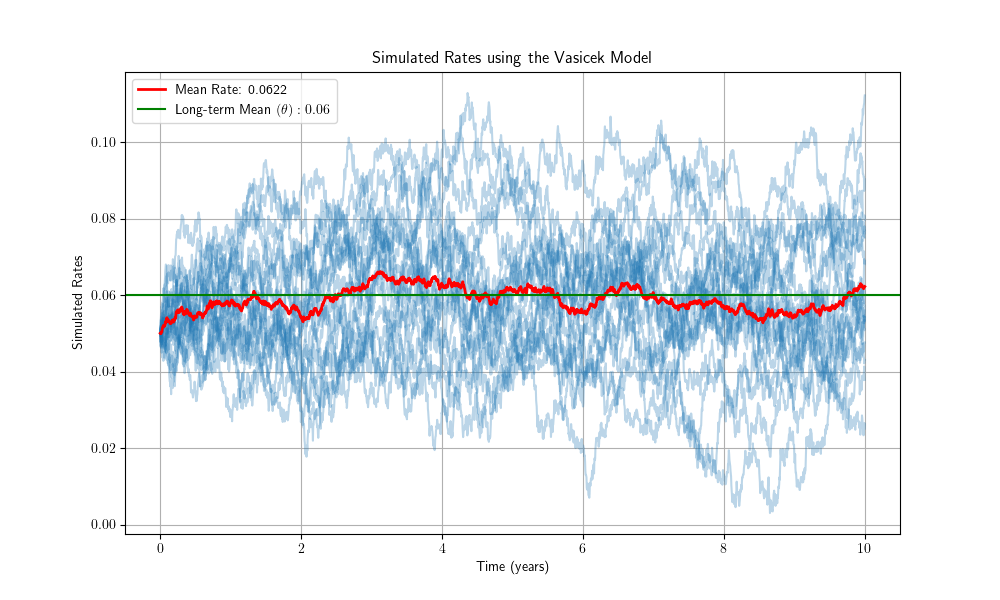
\includegraphics[width=0.75\linewidth]{/Users/nannaingemannohrt/Desktop/master_thesis/main/plots/VasicekModelPlotSIM.png}
    \caption{Plot of 10 simulated  rates  paths using the Vasicek model.}
    \label{fig:vasicek-sim}
\end{figure}
\noindent
Then we look closer at the dynamic of the short rate in \autoref{vas_dyn1}. This equation can be rearranged and integrated
to express the short rate, $r(t)$, as a function of its value at any prior time point s, 
so we have to have that for $s < t$ \cite{Bermudan}. 
\begin{align}
    d r_t &= \kappa \left[\theta - r(t)\right] dt + \sigma d W(t) \label{line_14} \\
    d r(t) &= k \theta dt - k r(t) dt + \sigma d W(t),  \\
    d r(t) + k r(t) dt &= k \theta dt + \sigma d W(t), \\
    e^{kt} d r(t) + k e^{kt} r(t) dt &= e^{kt} k \theta dt + e^{kt} \sigma d W(t), \\
    \frac{d}{dt} \left( e^{k t} r(t) \right) &= e^{k t} \frac{d}{dt} r(t) + k e^{k t} r_t dt, \\
    d\left( e^{k t} r(t) \right) &= e^{k t} dr(t) + k e^{k t} r_t dt, \\
    \int_s^t d \left( e^{ku} r(u) \right) &= k \theta \int_s^t e^{ku} du + \sigma \int_s^t e^{ku} d W(u), \\
    e^{kt} r(t) - e^{k s} r(s) &= \frac{k \theta}{k} \left( e^{kt} - e^{ks} \right) + \sigma \int_s^t e^{ku} d W(u), \\
    r(t) &= r(s) e^{-k(t-s)} + \theta \left( 1 - e^{-k(t-s)} \right) + \sigma \int_s^t e^{-k(t-u)} d W(u). \label{line_22}
\end{align}
From \autoref{line_14} to \autoref{line_22} the expression for the short rate in the Vasicek model is integrated, 
but first the terms in the stochastic differential equation is rearranged.
Then both sides of the equation are multiplied by the 
integrating factor $e^{\kappa t}$ to facilitate the integration. Next, both sides is integrated from s to t. The result of the
integration shows the change in the short  rate, r, over time, adjusted by the integrating factor. The final 
expression in \autoref{line_22} for the short rate, $r(t)$, at time t, showing how it depends on the initial rate, $r(s)$,
the mean-reverting term and the stochastic term \cite{Bermudan}. We note that  final expression in \autoref{line_22} for the short rate
is Gaussian.
\\\\
Further we find that $r(t)$ is normally distributed with mean and variance determined as follows \cite{Bjork}. 
\begin{align*}
    \EE \Big[r(t)\Big] & = \EE \Big[ r(s) e^{-k(t-s)} \Big] + \EE \Big[\theta \left( 1 - e^{-k(t-s)} \right)\Big]
    + \underset{:=0}{\underbrace{\EE \Big[\sigma \int_s^t e^{-k(t-u)} d W(u)\Big] }}\\
    & = \EE \Big[ r(s) e^{-k(t-s)} \Big] + \EE \Big[\theta \left( 1 - e^{-k(t-s)} \right)\Big] \\
    & = r(s) e^{-k(t-s)} + \theta \left( 1 - e^{-k(t-s)} \right) 
\end{align*}    
Using stochastic calculus, it can be demonstrated that the stochastic integral of a deterministic function 
$f(s)$ with respect to a Wiener process is distributed according to a Gaussian distribution,
having a mean of zero and a variance given by $\int_0^t f(s) ds$. We use this to find the variance of the short rate,
$r(t)$ \cite{Bjork}.
\begin{align*}
    Var\Big[r(t)\Big] &= Var\Big[\sigma \int_{s}^{t}e^{-k(t-u)} d W(u) \Big] \\
    &= \sigma^2 \int_{s}^{t}e^{-2k(t-u)} d W(u) \\
    &= \frac{\sigma^2}{2\kappa} \Big(e^{-2k(t-s)}\Big)
    \end{align*}
This lead to the theoretical distribution of the the short rate in the Vasicek model, which is represented below
\begin{align}
    R(t) \sim \mathcal{N} \Big[ r(s) e^{-k(t-s)} + \theta \left( 1 - e^{-k(t-s)} \right) ,
    \frac{\sigma^2}{2\kappa} \Big(e^{-2k(t-s)}\Big) \Big]
\end{align}
Moving towards simulating the distribution, we can use the above attributes of the short rate being Gaussian.
Given that the stochastic integral of a deterministic function with respect to a Wiener process is Gaussian distributed
with a mean of zero, we can simulate the short rate distribution by generating a large number of possible paths
for the Wiener process. Each path would then correspond to a realization of the short rate over time. In \autoref{fig:rates:hist}
below the described method is used and the simulated paths for the short rate in the Vasicek model and the distribution of one  the
simulated paths is plotted in a histogram. In \autoref{fig:rates:hist} the probability density function (PDF) of the 
fitted normal distribution is also plotted. This verifies that the short rate process in the Vasicek model is Gaussian distributed.
\begin{figure}[H]
    \centering
    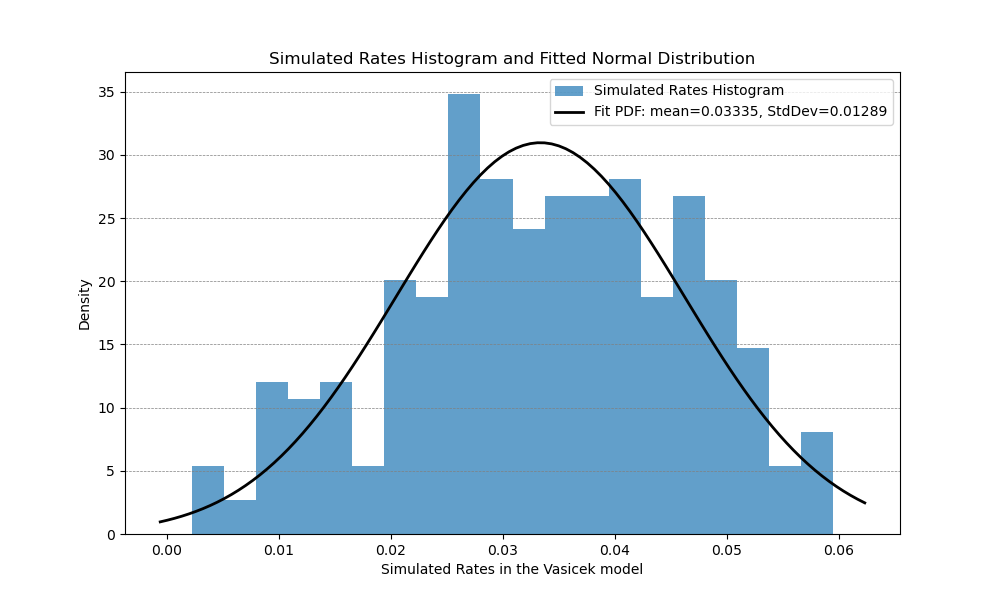
\includegraphics[width=0.75\textwidth]{/Users/nannaingemannohrt/Desktop/master_thesis/main/plots/NormalDistributionPlot.png}
    \caption{Histogram of one simulated rate path using the Vasicek model.}
    \label{fig:rates:hist}
\end{figure}
\noindent
Now some common properties of the Vasicek model has been reviewed and supported by simulations. Moving forward we will 
focus on bond prices using the Vasicek model. Earlier when we discussed bond prices, the Black Scholes model was introduced. 
\\\\
Now we will examine another aspect of the Vasicek model, namely the ability to derive explicit formulas
for bond pricing based on model expectations.
But first some words on how these bond prices are determined in the Vasicek model. 
When using the Vasicek model, it is possible to derive closed-form solutions for zero coupon bond prices. 
These prices are determined by an equation that factors in the current short rate, the speed of mean reversion,
the long-term mean level, the volatility of the short rate, and the bond’s time to maturity.
The bond prices formula from the Vasicek model considers the expected path of future short 
rates under the risk neutral measure, discounted back to the present value. 
\\\\
As mentioned we will now look a the formula for pricing bonds using the Vasicek model. We consider a zero coupon bond
with maturity T and at time t the price is given as in \autoref{price_zcb_vas} below \cite{Bjork}.
\begin{align}
    P(t,T) &= A(t,T) e^{-rB(t,T)} 
    \label{price_zcb_vas} 
\end{align}
Then we find the partial derivatives with respect to $r$ and $t$ of the zero coupon bond listed in \autoref{price_zcb_vas}.
\begin{align*}
    \frac{\partial P}{\partial t} &= \frac{\partial}{\partial t} (Ae^{-rB}) 
    = e^{-rB} \frac{\partial A}{\partial t} + Ae^{-rB} \frac{\partial}{\partial t} (-rB) \\
    &= e^{-rB} \frac{\partial A}{\partial t} - rAe^{-rB} \frac{\partial B}{\partial t} = 
    - \frac{P}{A} \frac{\partial A}{\partial t} - rP \frac{\partial B}{\partial t}
    \\\\
    \frac{\partial P}{\partial r} &= \frac{\partial}{\partial r} (Ae^{-rB}) 
    = Ae^{-rB} \frac{\partial}{\partial r} (-rB) = -PB 
    \\\\
    \frac{\partial^2 P}{\partial r^2} &= \frac{\partial}{\partial r} (-PB) = -B \frac{\partial}{\partial r} (P) = PB^2
\end{align*}
Then by applying Ito's lemma \cite{Bjork} and inserting the derivatives with respect to $r$ and $t$ we found above as well as
 the formula for the short rate in the Vasicek model present in \autoref{vas_dyn} we obtain the following
\begin{align*}
    dP(t,T) &= \frac{\partial P}{\partial t} dt + \frac{\partial P}{\partial r} dr 
    + \frac{1}{2} \frac{\partial^2 P}{\partial r^2} dr^2 \\
    dP(t,T) &= \left( \frac{P}{A} \frac{\partial A}{\partial t} - rP \frac{\partial B}{\partial t} \right) dt 
    + (-PB) dr + \frac{1}{2} (PB^2) dr^2 \\
    \frac{dP}{P} &= \left( \frac{1}{A} \frac{\partial A}{\partial t} - r \frac{\partial B}{\partial t} \right) dt 
    - B dr + \frac{1}{2} B^2 dr^2 \\
    \frac{dP}{P} &= \left( \frac{1}{A} \frac{\partial A}{\partial t} - r \frac{\partial B}{\partial t} \right) dt
     - B(\kappa \theta dt - \kappa r dt + \sigma dW_t) + \frac{1}{2} B^2 \sigma^2 dt\\
    \frac{dP}{P} &= \left( \frac{1}{A} \frac{\partial A}{\partial t} - r \frac{\partial B}{\partial t} 
    - \kappa \theta B + \kappa r B + \frac{1}{2} B^2 \sigma^2 \right) dt - \sigma B dW_t \\
\end{align*}
Under the risk neutral measure, the expected return of the bond must be equal to the risk free rate. Thus we have that
\begin{align*}
    r  &= \frac{1}{A} \frac{\partial A}{\partial t} - r \frac{\partial B}{\partial t} - \kappa \theta B 
    + \kappa r B + \frac{1}{2} B^2 \sigma^2  \\
    r \left( 1 + \frac{\partial B}{\partial t} - \kappa B \right) & =\frac{1}{A} \frac{\partial A}{\partial t} 
    - \kappa \theta B + \frac{1}{2} B^2 \sigma^2 
\end{align*}
Since this holds for all values of $r$, which does not feature in the left hand side, we deduce that
\begin{align}
    0 &= \frac{1}{A} \frac{\partial A}{\partial t} - \kappa \theta B + \frac{1}{2} B^2 \sigma^2 \label{equal_zero2}\\
    0 &=1 + \frac{\partial B}{\partial t} - \kappa B \label{equal_zero}
\end{align}
Considering that the price of zero coupon bond at maturity $P(T,T)=1$, the function $P=A e^{-rB}$ suggests $B(T,T)=0$
and $A(T,T)=0$. By then applying the integrating factor to the \autoref{equal_zero}, reorganizing and integrating
form t to T, we obtain
\begin{align}
   0 &= 1 + \frac{\partial B}{\partial t} - \kappa B \nonumber  \\
   0 &= e^{-\kappa t} + e^{-\kappa t} \frac{\partial B}{\partial t} - e^{-\kappa t} \kappa B \nonumber \\
   -e^{-\kappa t} &= e^{-\kappa t} \frac{\partial B}{\partial t} - e^{-\kappa t} \kappa B  \nonumber \\
   -e^{-\kappa t} dt &= d \left( e^{-\kappa t} B(t, T) \right) \nonumber \\
   - \int_{t}^{T} e^{-\kappa u} du &= \int_{t}^{T} d \left( e^{-\kappa t} B(t, T) \right) \nonumber  \\
   \frac{1}{\kappa} \left( e^{-\kappa T} - e^{-\kappa t} \right) &= e^{-\kappa T} B(T, T) - e^{-\kappa t} B(t, T)\nonumber  \\
   B(t,T) & =\frac{1}{\kappa} \left( 1 - e^{-\kappa (T-t)} \right)  
\end{align}
Finally  by substituting into \autoref{equal_zero2} and integrating we get that
\begin{align}
    0 &=\frac{1}{A} \frac{\partial A}{\partial t} - \kappa \theta B + \frac{1}{2} B^2 \sigma^2 \nonumber \\
    0 &= \frac{1}{A} \frac{\partial A}{\partial t} - \kappa \theta \left( \frac{1 - e^{-\kappa(T-t)}}{\kappa}
    \right) + \frac{\sigma^2}{2\kappa^2} \left( 1 - e^{-\kappa(T-t)} \right)^2 \nonumber \\
    0 &=  \frac{1}{A} \frac{\partial A}{\partial t} - \theta \left( 1 - e^{-\kappa(T-t)} \right) 
    + \frac{\sigma^2}{2\kappa^2} \left( 1 + e^{-2\kappa(T-t)} - 2e^{-\kappa(T-t)} \right)\nonumber \\
    \frac{1}{A} \frac{\partial A}{\partial t} &€= \theta \left( 1 - e^{-\kappa(T-t)} \right) 
    - \frac{\sigma^2}{2\kappa^2} \left( 1 + e^{-2\kappa(T-t)} - 2e^{-\kappa(T-t)} \right) \nonumber\\
    \int_{t}^{T} \frac{dA(u, T)}{A(u, T)} &= \theta \int_{t}^{T} \left(1 - e^{-\kappa(T-u)}\right) du 
    - \frac{\sigma^2}{2\kappa^2} \int_{t}^{T} \left(1 + e^{-2\kappa(T-u)} - 2e^{-\kappa(T-u)}\right) du \nonumber\\
    \ln A(T, T) - \ln A(t, T) &= \theta (T - t) - \theta \left(\frac{1 - e^{-\kappa(T-t)}}{\kappa} \right)
    - \frac{\sigma^2}{2\kappa^2} \left( (T - t) + \left(\frac{1 - e^{-2\kappa(T-t)}}{2\kappa}\right) 
    - 2\frac{1 - e^{-\kappa(T-t)}}{\kappa}\right) \nonumber\\
    -\ln A(t, T) &= \theta (T - t) - \theta \left(\frac{1 - e^{-\kappa(T-u)}}{\kappa} \right)
    - \frac{\sigma^2}{4\kappa^3} \left(2\kappa (T - t) + 1 - e^{-2\kappa(T-t)} - 4 + 4e^{-\kappa(T-t)}\right) \nonumber\\
    -\ln A(t, T) &= \theta (T - t) - \theta \left(\frac{1 - e^{-\kappa(T-u)}}{\kappa} \right)
    - \frac{\sigma^2}{4\kappa^3} \left(2\kappa (T - t) - \left(1 + e^{-2\kappa(T-t)} 
    - 2e^{-\kappa(T-t)}\right) - 2 + 2e^{-\kappa(T-t)}\right) \nonumber\\
    -\ln A(t, T) &= \theta (T - t) - \theta \left(\frac{1 - e^{-\kappa(T-u)}}{\kappa}\right) - \frac{\sigma^2}{2 \kappa^2}
    \left((T-t)- \frac{1-e^{-\kappa(T-t)}}{\kappa}\right) + \frac{\sigma^2}{4 {\kappa}^3}\left(1-e^{-\kappa(T-t)}\right)^2 \nonumber\\
    \ln A(t, T) &= \left(\theta -\frac{\sigma^2}{2\kappa^2}\right) \left(\frac{1-e^{-\kappa(T-u)}}{\kappa}-(T-t)\right)
    -\frac{\sigma^2}{4 \kappa}\left(\frac{1-e^{-\kappa(T-t)}}{\kappa}\right)^2 \nonumber\\
    A(t,T)&= \exp \Biggl\{\left(\theta-\frac{\sigma^2}{2 \kappa^2}\right)\left(\frac{1-e^{-\kappa(T-u)}}{\kappa}-(T-t)\right)
    -\frac{\sigma^2}{4 \kappa}\left(\frac{1-e^{-\kappa(T-t)}}{\kappa}\right)^2 \Biggr\} 
\end{align}
\\\\
 Combining this we get the formula for pricing bonds using the Vasicek model, which present 
 in Proposition \autoref{prop 5} below. 
\newpage
\begin{proposition}
    \label{prop 5}
    \textbf{(The Vasicek term structure)} In the Vasicek model, bond prices are given by
 \begin{align}
    P(t,T) &= A(t,T) e^{-rB(t,T)} 
\end{align}
where
\begin{align*}
    A(t,T)&= \exp \Biggl\{\left(\theta-\frac{\sigma^2}{2 \kappa^2}\right)\left(\frac{1-e^{-\kappa(T-u)}}{\kappa}-(T-t)\right)
    -\frac{\sigma^2}{4 \kappa}\left(\frac{1-e^{-\kappa(T-t)}}{\kappa}\right)^2 \Biggr\} \\
    B(t,T) & =\frac{1}{\kappa} \left( 1 - e^{-\kappa (T-t)} \right)  
\end{align*}
\cite{Bjork}

\end{proposition}
\noindent
To illustrate the behavior of bond price in the Vasicek model, a small simulation study is performed. For the study 
some parameters are chosen, these are listed in \autoref{tab:parameters_zcb}. In \autoref{fig:zcb_sim_1_plot} one simulate
path for the development of the ZCB price is illustrated and in \autoref{fig:zcb_sim_10_plot} ten simulated paths are illustrated.
We see that the price fluctuate over the price period, as expected.
\\
\begin{table}[H]
    \centering
    \begin{tabular}{ccc}
      \toprule
      \textbf{Parameter} & \textbf{Parameter explanation} & \textbf{Value} \\
      \midrule
      \rowcolor{lightgray!40} $T$ & Time to maturity & 10 \\
      $r_0$ & Initial short rate & Simulated \\
      \rowcolor{lightgray!40} $\kappa$ & Mean reversion speed & 0.2\\
      $\theta$ & Long-term average rate  & 0.03 \\
      \rowcolor{lightgray!40} $\sigma$ & Volatility& 0.02 \\
      \bottomrule
    \end{tabular}
    \caption{Summary of parameters used simulation ZCB prices in the Vasicek model}
    \label{tab:parameters_zcb}
\end{table}
\noindent
\begin{figure}[H]
    \centering
    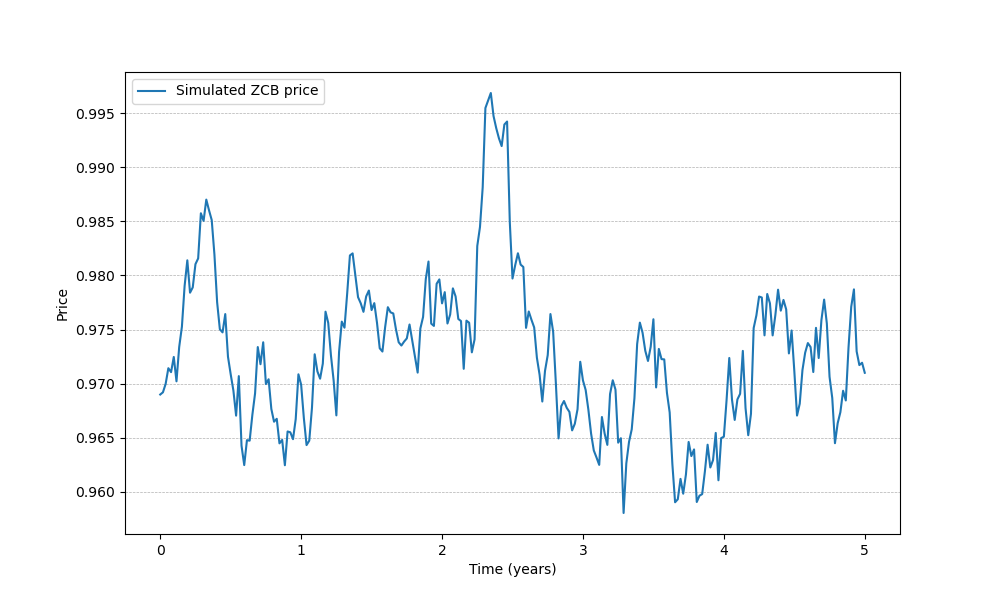
\includegraphics[width=0.75\linewidth]{/Users/nannaingemannohrt/Desktop/master_thesis/main/plots/zcb_1_sim.png}
    \caption{Plot of one simulated ZCB price path using the Vasicek model.}
    \label{fig:zcb_sim_1_plot}
\end{figure}
\noindent
\begin{figure}[H]
    \centering
    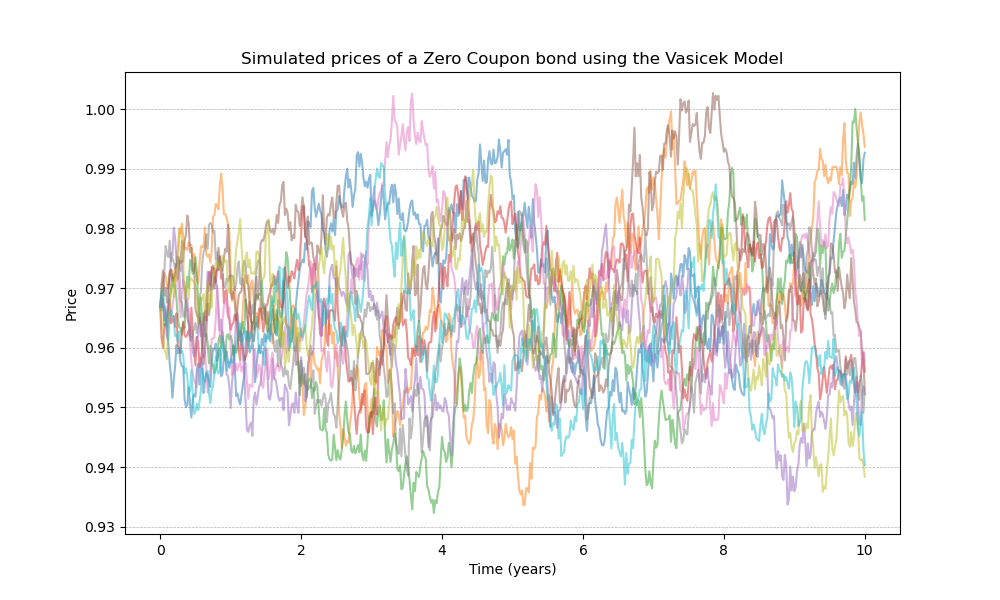
\includegraphics[width=0.75\linewidth]{/Users/nannaingemannohrt/Desktop/master_thesis/main/plots/zcb_10_sim.png}
    \caption{Plot of 10 simulated  ZCB prices  paths using the Vasicek model.}
    \label{fig:zcb_sim_10_plot}
\end{figure}
\noindent
The Vasicek model has now been introduced and we have taken a closer look at the distribution in the short rate model. 
This examination leads us to the Vasicek term structure model, which outlines the method for pricing bonds using the 
Vasicek framework. Similarly, in Chapter 3, specific decisions are made regarding the calculation of bond prices with 
the Vasicek model. A critical decision is the assumption that the volatility, 
$\sigma$, is a positive constant. However, we should consider whether volatility remains constant over a given period.
\\\\
Subsequently, we will introduce another model, the SABR (Stochastic Alpha, Beta, Rho) model. The SABR model is a stochastic volatility model 
utilized to estimate the implied volatility smile. Although it does not provide a direct formula for option pricing, 
the estimated implied volatility curve can be employed in the Black Scholes model, discussed earlier, to price swaptions. 
Before we dig into the SABR model, we will examine the assumption of constant volatility inherent in the Black Scholes model.
The purpose of this small analysis, it to make an attachment to the
market and see some examples of not constant volatility. This can 
be seen as a motivation for looking into two-factor models, 
instead of a one-factor model, like the Vasicek model. 

\newpage
\section{Constant Volatility} \label{cont_vol}
This chapter will look into the limitations 
of the Black Scholes model, particularly its 
assumption of constant volatility, and introduce 
the SABR model as a more dynamic alternative for estimating volatility. 
The chapter will illustrate the inconsistency of 
this assumption with real-world market data, 
using the S$\&$P 500 index and the 10Y10Y EUR swaption 
as examples.
\\\\
The Black Scholes model, introduced earlier, outlines the pricing formula for an European call option in 
Proposition \autoref{Black-Scholes Formula}. It is  essential to recall that in the Black Scholes formula, 
volatility is considered constant. This implies that the volatility of the asset's returns does not vary over time,
establishing a direct correlation between the option's price and its volatility. Consequently, 
understanding implied volatility becomes crucial. Although the Black Scholes model does not provide 
a closed-form solution for implied volatility, it can be determined numerically, a topic not covered 
in this analysis. Instead, we introduce the SABR model to estimate volatility, which can then be 
applied to the Black Scholes model for option pricing. This will be covered in the Section \ref{SABR_model} about the 
SABR model. 
\\\\
We will briefly demonstrate why the assumption of constant volatility is inconsistent with market data. 
Our analysis includes an examination of the S$\&$P 500 index and a 10Y10Y EUR swaption, which are frequently used 
financial indicators. 
\\\\
As depicted in \autoref{10Y10Y dev} and \autoref{sp500 dev}, the development of the 10Y10Y EUR swaption 
and S$\&$P 500 index levels illustrates fluctuations over time. This variability is further emphasized by the return patterns 
shown in \autoref{10Y10Y return} and \autoref{sp500 return}, where the returns of the 10Y10Y EUR swaption and S$\&$P 500 index are plotted. 
These fluctuations suggest that market volatility is not constant. Our analysis underlines that volatility varies 
significantly from day to day, reflecting the market's response to new information and events. This observation challenges 
the applicability of the Black Scholes model, which assumes constant volatility and highlights the need for models like the 
SABR model that more accurately capture market dynamics and provide nuanced volatility estimates.
\begin{figure}[H]
    \centering
    \begin{minipage}{0.5\textwidth}
        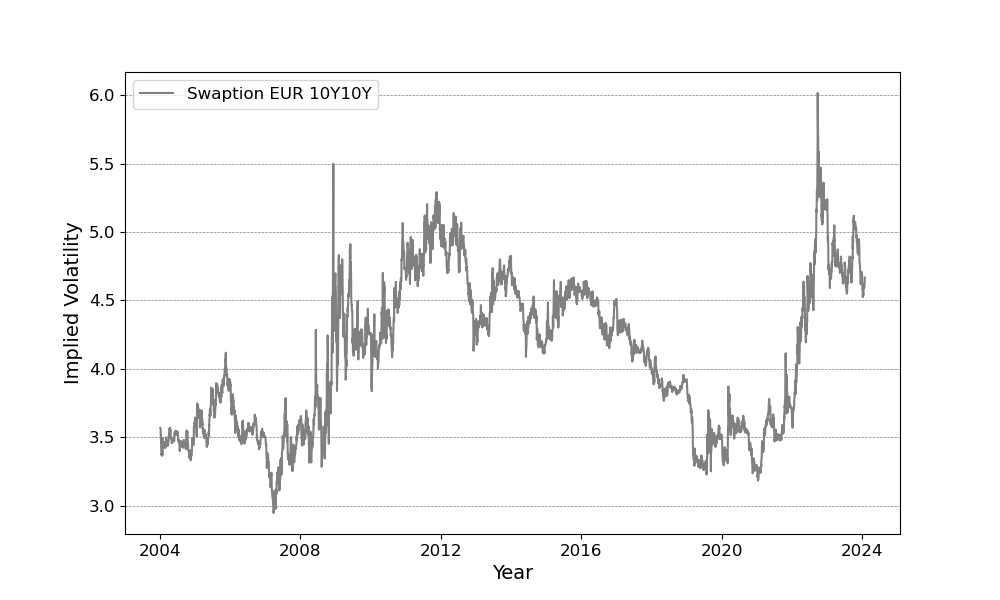
\includegraphics[width=\linewidth]{/Users/nannaingemannohrt/Desktop/master_thesis/main/plots/10Y10Yswaption.png}
        \caption{Swaption EUR 10Y10Y from 01.01.2004 \\ to 01.01.2024. Data source Citi Velocity }
        \label{10Y10Y dev}
    \end{minipage}\hfill 
    \begin{minipage}{0.5\textwidth}
        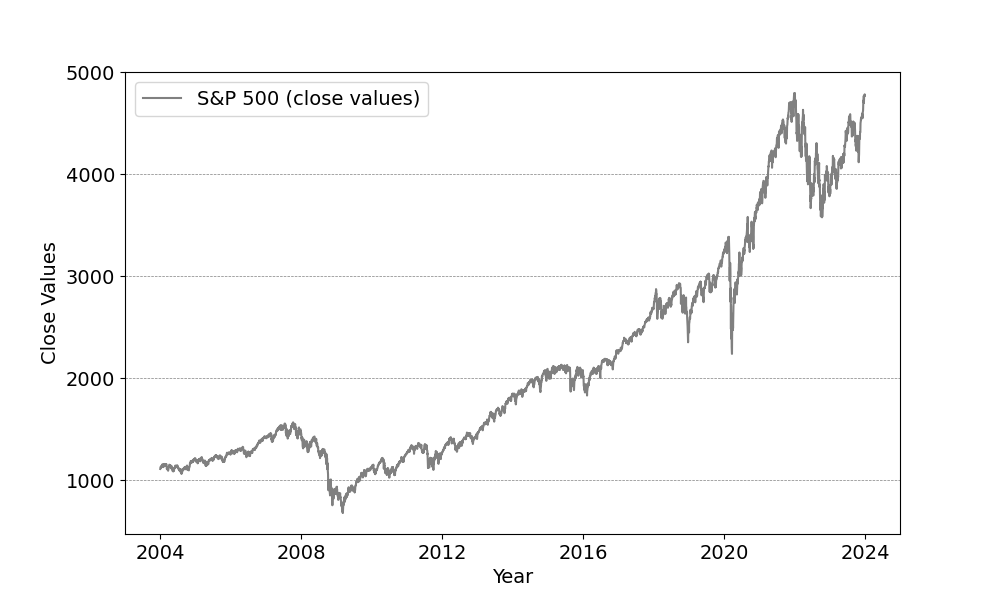
\includegraphics[width=\linewidth]{/Users/nannaingemannohrt/Desktop/master_thesis/main/plots/sp500.png}
        \caption{S$\&$P500 index (close values) from \\ 01.01.2004 to 01.01.2024. Data source Yahoo Finance. }
        \label{sp500 dev}
    \end{minipage}
\end{figure}

\begin{figure}[H]
    \centering
    \begin{minipage}{0.5\textwidth}
        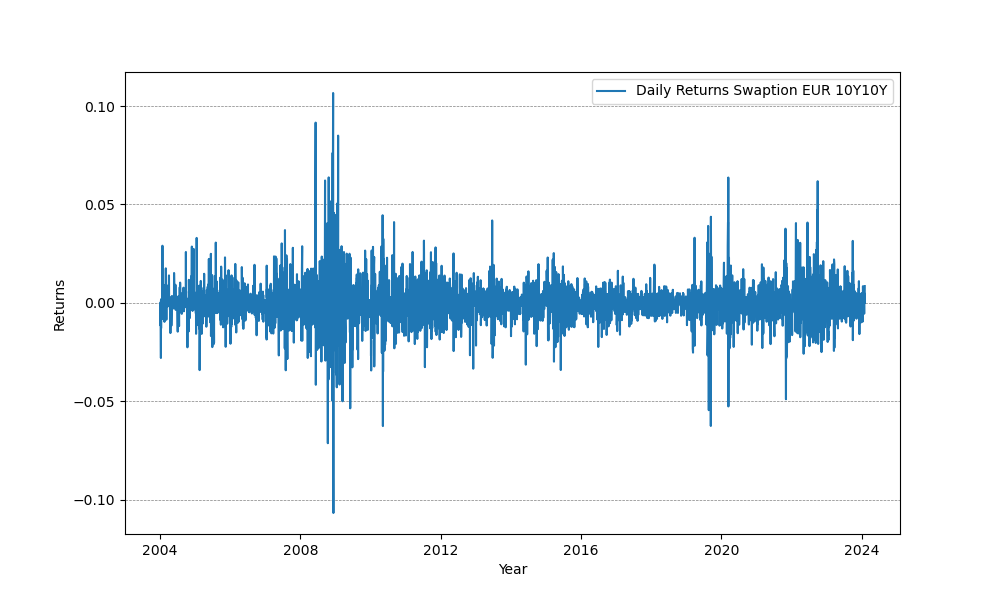
\includegraphics[width=\linewidth]{/Users/nannaingemannohrt/Desktop/master_thesis/main/plots/10Y10Yswaptionreturn.png}
        \caption{Swaption EUR 10Y10Y return from  \\ 01.01.2004 to 01.01.2024.}
        \label{10Y10Y return}
    \end{minipage}\hfill 
    \begin{minipage}{0.5\textwidth}
        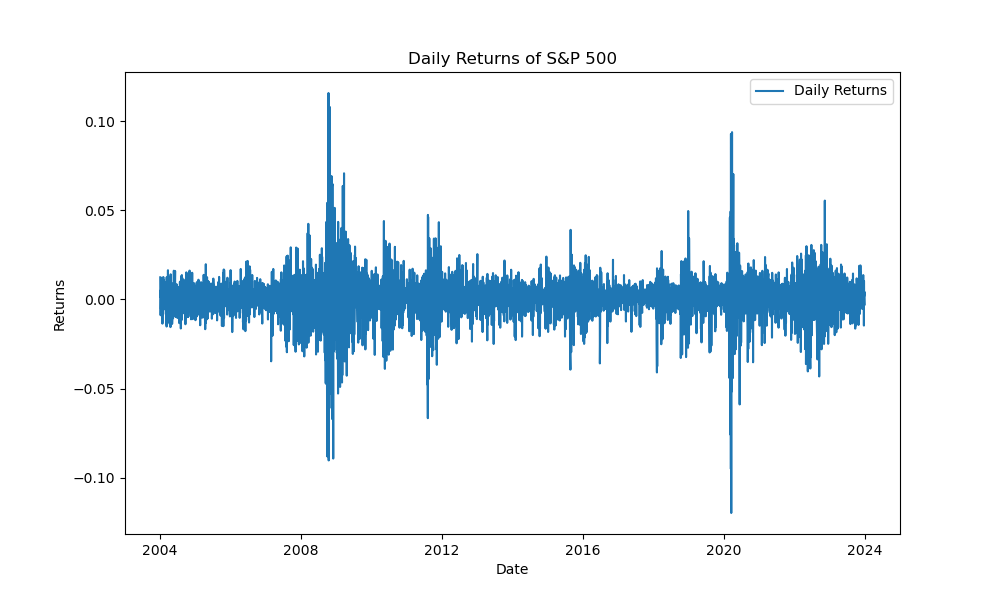
\includegraphics[width=\linewidth]{/Users/nannaingemannohrt/Desktop/master_thesis/main/plots/sp500return.png}
        \caption{S$\&$P500 index (close values) return  \\ from 01.01.2004 to 01.01.2024.}
        \label{sp500 return}
    \end{minipage}
\end{figure}
\noindent
The market data reveals a tendency in 
volatility, indicating that it is not constant. 
Given this fluctuation, how should we proceed when 
considering to be able to price a swaption? We will continue our 
analysis by exploring a two-factor model rather 
than the previously described one-factor Vasicek model. 
This approach allows us to model volatility 
stochastically and use the resulting volatility 
estimates to price a swaption in the Black Scholes model. 

\newpage
\section{Data} \label{data_lab}
In Chapter \ref{cont_vol} wee looked into the assumption of constant volatility in the Black-Scholes model. 
Where during the study, a 10Y10Y EUR swaption was introduced. This chapter will provide a introduction to 
market data on swaptions. In this thesis the data source is Citi Velocity, which is a market data plantformed
owned by Citi Bank.
\\\\
Before delving into the market data on swaptions, let's revisit the definition of a swaption. 
A swaption gives the holder the right, but not the obligation, to enter into an interest rate swap in the future. 
There are two types of swaptions: payer swaptions and receiver swaptions, as previously described.
\\\\
The four main parameters defining a swaption are:
\begin{itemize}
\item \textbf{Expiry} \text{---}  when in the future the holder can exercise their right.
\item \textbf{Tenor} \text{---}  the maturity of the underlying interest rate swap.
\item \textbf{Strike} \text{---}  the pre-specified interest rate of the swap.
\item \textbf{Pay/Receive} \text{---}  whether the holder pays or receives the fixed rate.
\end{itemize}
\noindent
As mentioned a 10Y10Y EUR swaption was analyzed, but let's clarify what a 10Y10Y EUR swaption entails. 
Assuming the swaption is a receiver swaption, it represents a contract that, in ten years, 
gives the holder the right to enter into a ten year interest rate swap in EUR, receiving a fixed rate. 
Thus, the swaption has an expiry of 10 years, a tenor of 10 years, and a strike equivalent to the value of the fixed rate. 
It is important to note that the underlying interest rate swap in the swaption is a forward swap, commencing 10 years from now: 
the settlement date.
\\\\
Then before we will look at some displayed data, let's first cover some lingo of swaption. 
A swaption with a strike set at the current market rate for the underlying forward swap is referred 
to as at-the-money-forward (ATMF). If the strike differs from the ATMF rate, the swaption is categorized as out-of-the-money (OTM).
\newpage
\noindent
When discussing swaptions, it is essential to recognize how the volatility surface or smile varies across different expiries and swap 
forward tenors. Displayed below in \autoref{tab:swaption_skew_ATMF} is the ATMF swaption volatility surface. 
The presentation of the volatility surface in swaptions differs notably from that in other asset classes like equities. 
In the case of equities, different tenors are not a consideration, allowing both at-the-money (ATM) and out-of-the-money (OTM) 
levels to be represented on a single chart. Conversely, the out-of-the-money-forward (OTMF) swaption volatility surface, 
as shown in \autoref{tab:swaption_skew_OTMF}, adopts a different layout. The horizontal axis of 
\autoref{tab:swaption_skew_OTMF} spans a range of strikes, from -200 basis points below to +200 basis points above the ATM strike.
\\\\
Now a short introduction to swaption data has been covered, then the next step is to illustrated some 
volatility surface. The purpose of during this is first of all, to underline that the volatility surface for a 
given swaption change over time. Secondly it is to see that the volatility smile for swaption with a fixed
expiry and various tenor can also be slightly different.  From \autoref{fig:rates:smile_5} we see the volatility surface
for a 10Y10Y EUR swaption at five days over the time period from 20.02.2020 to 20.02.2024. From the plot 
we clearly see that the volatility surface is change over the period. We see a pattern of the volatility surface moving 
up and down, without large change in the curvature of the volatility surface. This implies changes in the alpha or beta parameter
i the SABR, which will be covered later in Chapter \ref{invest_sabr}. Then we look at the OTM volatility surface
where the swaption expiry is fixed at ten years, but for various tenors. We look at this case over to days, where the first 
on the dates 20.02.2023 and 20.02.2024. This leads to at plot for each combination of the fixed expiry (10Y) and the various tenor. 
These volatility surface plots is illustrated in \autoref{fig:10Y1Y_} to \autoref{fig:10Y30Y_} below.
These plots clearly show changes in the volatility surface across different tenors. 
The volatility surface becomes flatter and more symmetric around the ATM strike for longer tenors, 
indicating a shift in the parameter nu, which measures the volatility of volatility. We will discuss 
this further in \ref{invest_sabr}.
\\
\begin{table}[H]
    \centering
    \scalebox{1}{
    \begin{tabular}{|c|c|c|c|c|c|c|c|c|c|}
    \hline  
        \multicolumn{10}{|c|}{Tenor} \\ 
    \hline
     Expiry& 1Y & 2Y & 3Y & 5Y & 7Y & 10Y & 15Y & 20Y & 30Y \\
    \hline
    \rowcolor{lightgray!40} 1M & 5.2896 & 6.0865 & 5.9731 & 5.6770 & 5.4074 & 5.0402 & 4.8121 & 4.6578 & 4.5098 \\
    2M & 5.4361 & 6.1242 & 5.9983 & 5.7206 & 5.4838 & 5.1569 & 4.9592 & 4.7942 & 4.6228 \\
    \rowcolor{lightgray!40} 3M & 5.5244 & 6.1032 & 5.9953 & 5.7530 & 5.5240 & 5.1959 & 5.0318 & 4.8662 & 4.6948 \\
    6M & 6.0007 & 6.3187 & 6.1810 & 5.9009 & 5.7098 & 5.4304 & 5.2822 & 5.1272 & 4.9696 \\
    \rowcolor{lightgray!40} 9M & 6.2264 & 6.3990 & 6.2515 & 6.0103 & 5.8553 & 5.6185 & 5.4686 & 5.3155 & 5.1284 \\
    12M & 6.2698 & 6.3692 & 6.2157 & 6.0080 & 5.8713 & 5.6575 & 5.4984 & 3.5614 & 5.1749 \\
    \rowcolor{lightgray!40} 18M & 6.3333 & 6.3395 & 6.2046 & 6.0073 & 5.8874 & 5.7166 & 5.5284 & 5.3998 & 5.2215 \\
    2Y & 6.2967 & 6.2853 & 6.1613 & 5.9773 & 5.8477 & 5.7289 & 5.5014 & 5.3854 & 5.2146 \\
    \rowcolor{lightgray!40} 3Y & 6.1824 & 6.1546 & 6.0463 & 5.8606 & 5.7536 & 5.6654 & 5.4234 & 5.2916 & 5.1171 \\
    4Y & 6.0380 & 6.0008 & 5.8975 & 5.7407 & 5.6613 & 5.5681 & 5.3010 & 5.1479 & 4.9677 \\
    \rowcolor{lightgray!40} 5Y & 5.8966 & 5.8683 & 5.7524 & 5.6119 & 5.5376 & 5.4563 & 5.1646 & 5.0015 & 4.8213 \\
    7Y & 5.6398 & 5.6152 & 5.5170 & 5.3796 & 5.2946 & 5.2228 & 4.9248 & 4.7421 & 4.5575 \\
    \rowcolor{lightgray!40} 10Y & 5.3399 & 5.3311 & 5.2101 & 5.0614 & 4.9531 & 4.8315 & 4.5247 & 4.3559 & 4.1757 \\
    12Y & 5.1687 & 5.1598 & 5.0635 & 4.8726 & 4.7460 & 4.5879 & 4.2716 & 4.1312 & 3.9422 \\
    \rowcolor{lightgray!40} 15Y & 4.9532 & 4.9412 & 4.8215 & 4.5966 & 4.4391 & 4.2880 & 3.9736 & 3.8382 & 3.6523 \\
    20Y & 4.5909 & 4.5840 & 4.4649 & 4.2116 & 4.0605 & 3.8790 & 3.5666 & 3.4626 & 3.2743 \\
    \rowcolor{lightgray!40} 30Y & 4.1109 & 4.1065 & 3.9893 & 3.6882 & 3.5119 & 3.2952 & 3.0168 & 2.9317 & 2.7602 \\
    \hline
    \end{tabular}
    }
    \caption{At-the-money-forward (ATMF) swaption volatility surface. Normal absolute values. Data source Citi Velocity 20.02.2024. }
    \label{tab:swaption_skew_ATMF}
\end{table}

\begin{table}[H]
    \centering
    \scalebox{0.9}{
    \begin{tabular}{|c|c|c|c|c|c|c|c|c|c|c|c|}
        \hline  
            \multicolumn{12}{|c|}{Strike} \\ 
        \hline
        Expiry x Tenor& -200   & -100   & -75    & -50    & -25    & \textbf{ATM}    & 25     & 50     & 75     & 100    & 200    \\ 
        \hline
        \rowcolor{lightgray!40} 10Y x 1Y  & 5.1416 & 5.1819 & 5.2105 & 5.2465 & 5.2898 & \textbf{5.3399} & 5.3966 & 5.4596 & 5.5283 & 5.6025 & 5.9448 \\
        10Y x 2Y  & 5.1588 & 5.1864 & 5.2116 & 5.2442 & 5.2841 & \textbf{5.3311} & 5.3845 & 5.4444 & 5.5102 & 5.5815 & 5.9138 \\
        \rowcolor{lightgray!40} 10Y x 3Y  & 5.0699 & 5.0806 & 5.1017 & 5.1304 & 5.1665 & \textbf{5.2101} & 5.2599 & 5.3166 & 5.3795 & 5.4480 & 5.7709 \\
        10Y x 5Y  & 4.9781 & 4.9597 & 4.9735 & 4.9950 & 5.0241 & \textbf{5.0614} & 5.1043 & 5.1549 & 5.2119 & 5.2750 & 5.5792 \\
        \rowcolor{lightgray!40} 10Y x 7Y  & 4.9234 & 4.8694 & 4.8762 & 4.8916 & 4.9157 & \textbf{4.9531} & 4.9896 & 5.0388 & 5.0955 & 5.1594 & 5.4749 \\
        10Y x 10Y & 4.8882 & 4.7796 & 4.7750 & 4.7806 & 4.7966 & \textbf{4.8315} & 4.8598 & 4.9065 & 4.9626 & 5.0275 & 5.3610 \\
        \rowcolor{lightgray!40} 10Y x 12Y & 4.7487 & 4.6379 & 4.6305 & 4.6334 & 4.6170 & \textbf{4.6781} & 7.7064 & 4.7517 & 4.8068 & 4.8709 & 5.2033 \\
        10Y x 15Y & 4.6292 & 4.4963 & 4.4859 & 4.4862 & 4.4974 & \textbf{4.5247} & 4.5530 & 4.5970 & 4.6509 & 4.7143 & 5.0457 \\
        \rowcolor{lightgray!40}10Y x 20Y & 4.4983 & 4.3478 & 4.3329 & 4.3288 & 4.3360 & \textbf{4.3559} & 4.3846 & 4.4256 & 4.4772 & 4.5385 & 4.8650 \\
        10Y x 30Y & 4.3647 & 4.1915 & 4.1706 & 4.1605 & 4.1619 & \textbf{4.1757} & 4.2003 & 4.2370 & 4.2847 & 4.3428 & 4.6603 \\ 
        \hline
 \end{tabular}
    }
    \caption{Out-of-the-money-forward (OTMF) swaption volatility surface. Normal absolute values.  Data source Citi Velocity  21.02.2024. }
    \label{tab:swaption_skew_OTMF}
\end{table}

\begin{figure}[H]
    \centering
    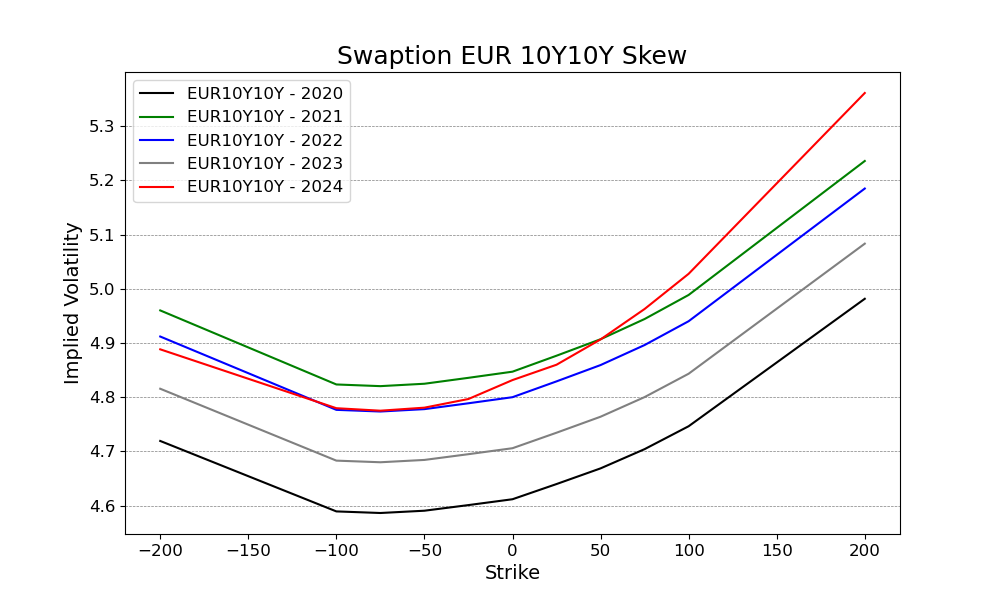
\includegraphics[scale =0.6]{/Users/nannaingemannohrt/Desktop/master_thesis/main/plots/10Y10Y_4_smiles.png}
    \caption{EUR swaption 10Y10Y skew over five years. Data source Citi Velocity.}
    \label{fig:rates:smile_5}
\end{figure}

\newpage
\begin{figure}[H]
    \centering
    \begin{subfigure}{0.43\textwidth}
        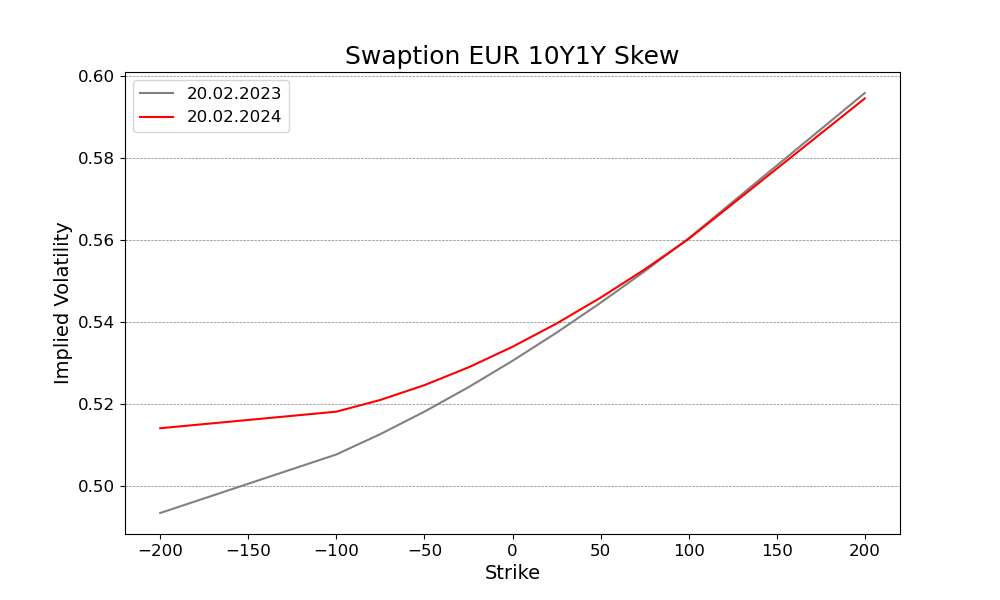
\includegraphics[scale =0.22]{/Users/nannaingemannohrt/Desktop/master_thesis/main/plots/10Y1Y.png}
        \caption{Volatility Surface EUR swaption 10Y1Y}
        \label{fig:10Y1Y_}
    \end{subfigure}\hfill
    \begin{subfigure}{0.43
        \textwidth}
        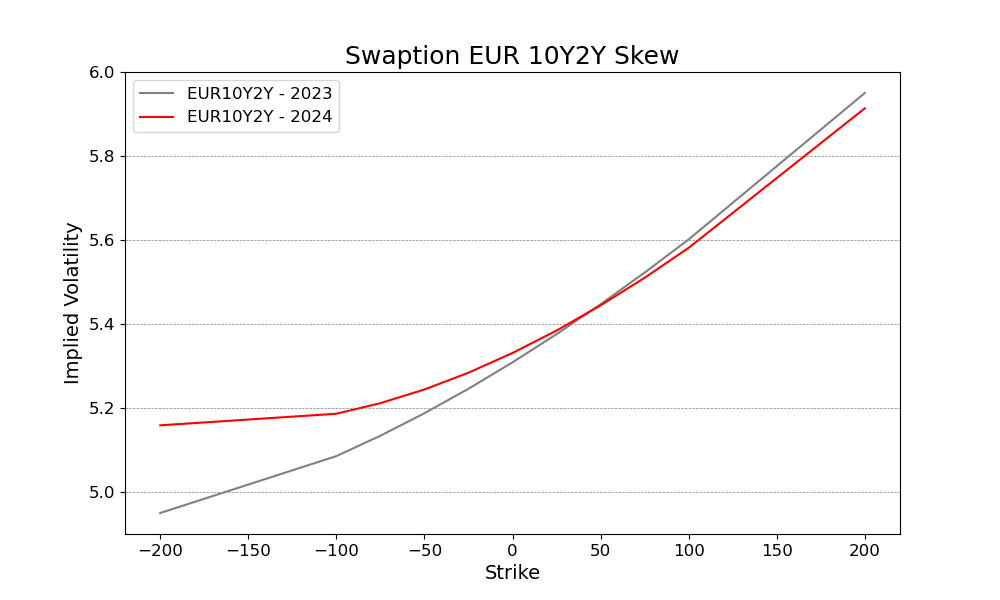
\includegraphics[scale =0.22]{/Users/nannaingemannohrt/Desktop/master_thesis/main/plots/10Y2Y.png}
        \caption{Volatility Surface EUR swaption 10Y2Y}
        \label{fig:10Y2Y_}
    \end{subfigure}
    \begin{subfigure}{0.43\textwidth}
        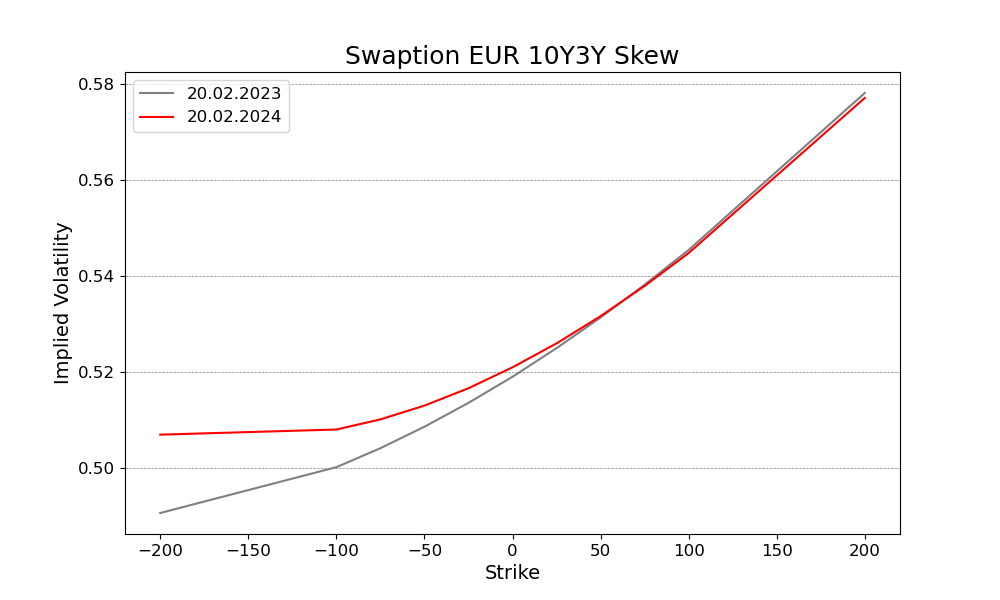
\includegraphics[scale =0.22]{/Users/nannaingemannohrt/Desktop/master_thesis/main/plots/10Y3Y.png}
        \caption{Volatility Surface EUR swaption 10Y3Y}
        \label{fig:10Y3Y_}
    \end{subfigure}\hfill
    \begin{subfigure}{0.43\textwidth}
        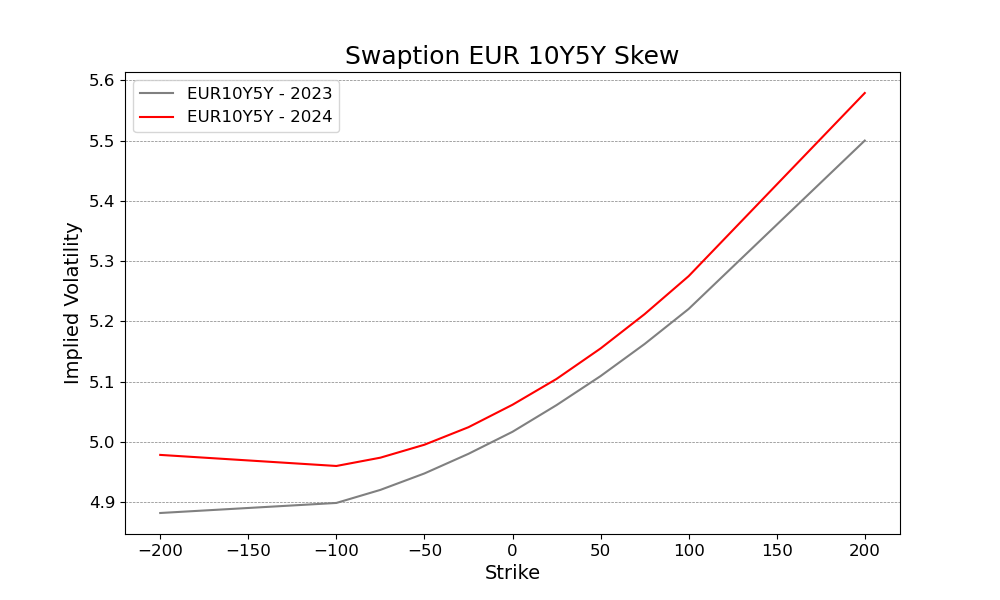
\includegraphics[scale =0.22]{/Users/nannaingemannohrt/Desktop/master_thesis/main/plots/10Y5Y.png}
        \caption{Volatility Surface EUR swaption 10Y5Y}
        \label{fig:10Y5Y_}
    \end{subfigure}
    \begin{subfigure}{0.43\textwidth}
        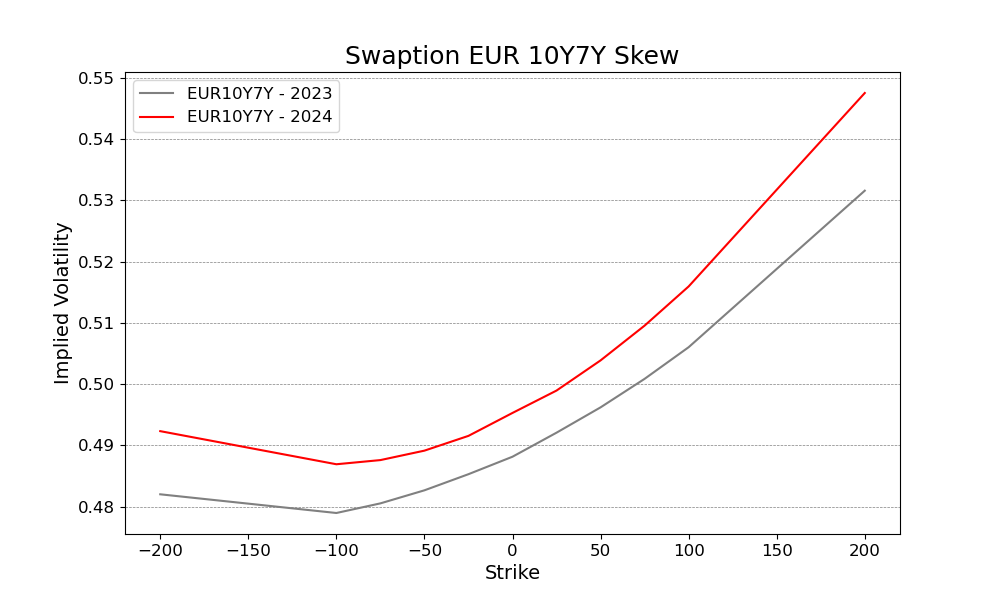
\includegraphics[scale =0.22]{/Users/nannaingemannohrt/Desktop/master_thesis/main/plots/10Y7Y.png}
        \caption{Volatility Surface EUR swaption 10Y7Y}
        \label{fig:10Y7Y_}
    \end{subfigure}\hfill
    \begin{subfigure}{0.43\textwidth}
        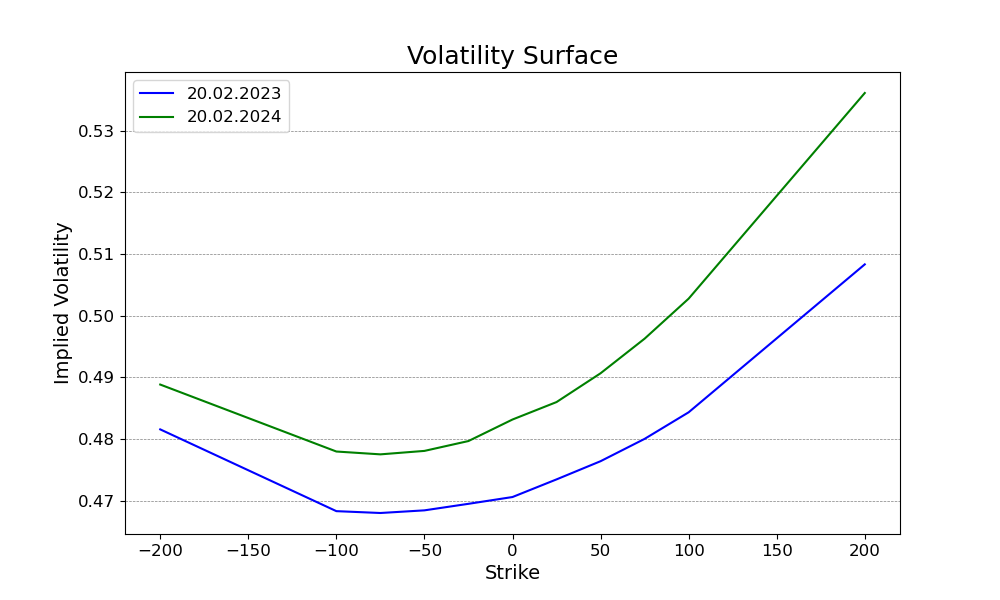
\includegraphics[scale =0.22]{/Users/nannaingemannohrt/Desktop/master_thesis/main/plots/10Y10Y.png}
        \caption{Volatility Surface EUR swaption 10Y10Y}
        \label{fig:10Y10Y_}
    \end{subfigure}

    \begin{subfigure}{0.43\textwidth}
        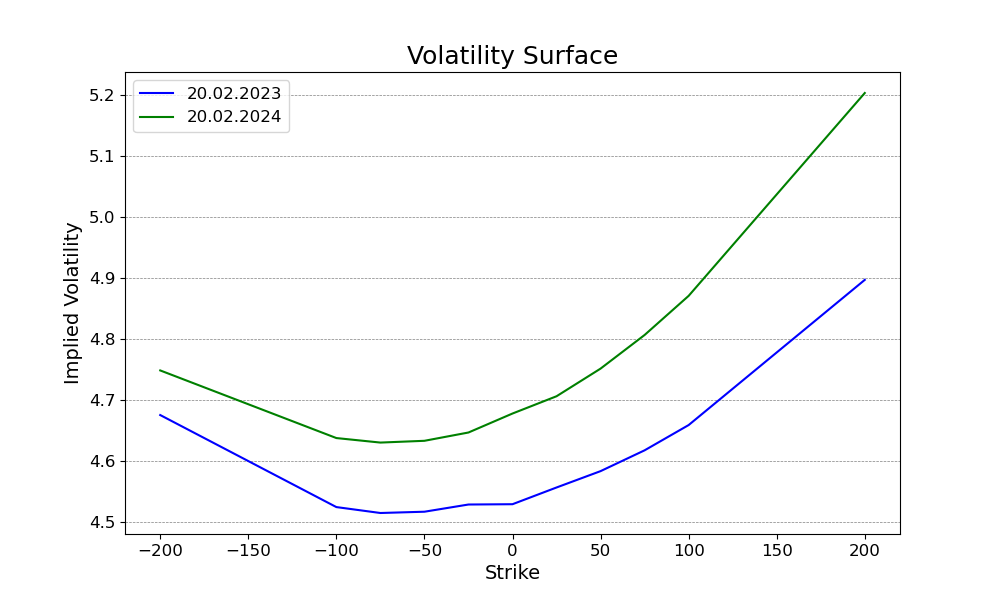
\includegraphics[scale =0.22]{/Users/nannaingemannohrt/Desktop/master_thesis/main/plots/10Y12Y.png}
        \caption{Volatility Surface EUR swaption 10Y12Y}
        \label{fig:10Y12Y_}
    \end{subfigure}\hfill
    \begin{subfigure}{0.43\textwidth}
        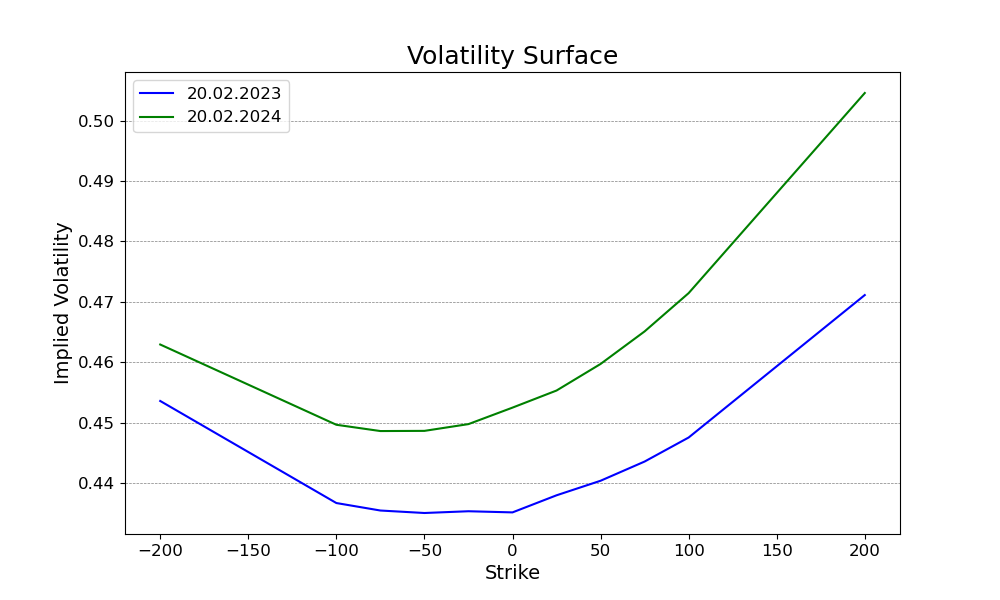
\includegraphics[scale =0.22]{/Users/nannaingemannohrt/Desktop/master_thesis/main/plots/10Y15Y.png}
        \caption{Volatility Surface EUR swaption 10Y15Y}
        \label{fig:10Y15Y_}
    \end{subfigure}
    \begin{subfigure}{0.43\textwidth}
        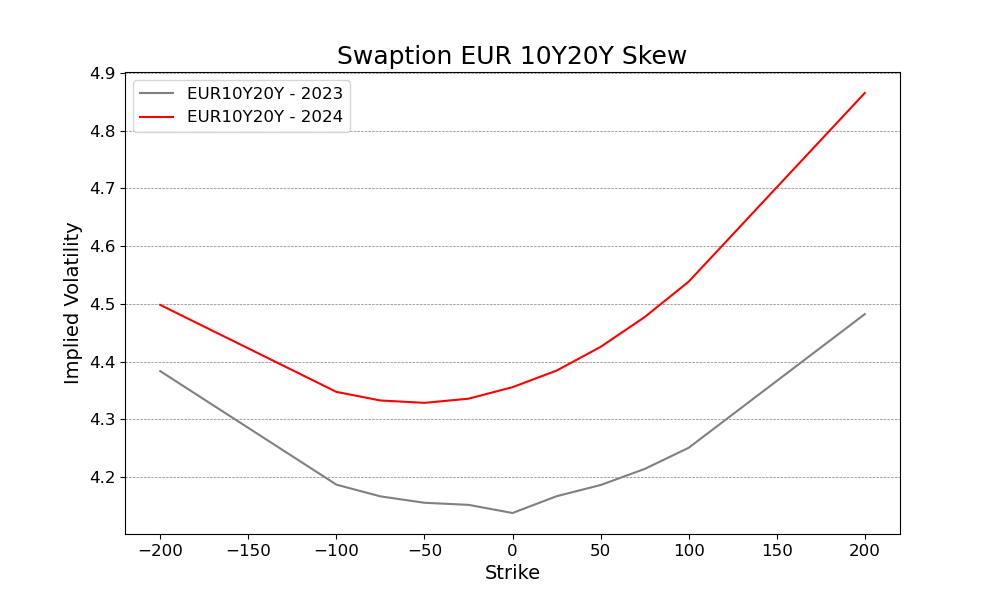
\includegraphics[scale =0.22]{/Users/nannaingemannohrt/Desktop/master_thesis/main/plots/10Y20Y.png}
        \caption{Volatility Surface EUR swaption 10Y20Y}
        \label{fig:10Y20Y_}
    \end{subfigure}\hfill
    \begin{subfigure}{0.43\textwidth}
        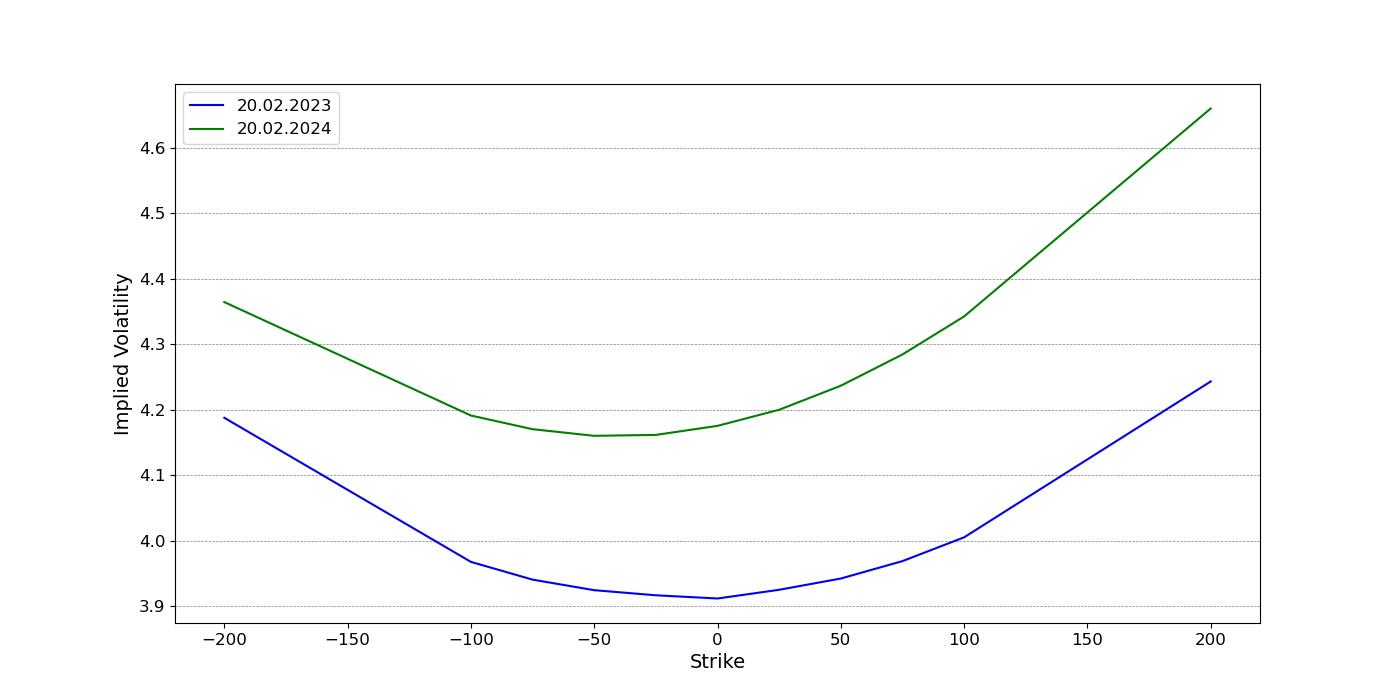
\includegraphics[scale =0.22]{/Users/nannaingemannohrt/Desktop/master_thesis/main/plots/10Y30Y.png}
        \caption{Volatility Surface EUR swaption 10Y30Y}
        \label{fig:10Y30Y_}
    \end{subfigure}
\end{figure}   

\newpage
\section{ The SABR Model} \label{SABR_model}
In this Chapter, we will first introduce the SABR model
 and explain how to determine the forward rate and 
 volatility using this model. We will then focus on 
 calculating implied volatility and pricing European 
 options with the SABR model. Finally, the Chapter 
 will discuss methods for estimating the parameters 
 of the SABR model.
\\\\
The SABR (Stochastic Alpha, Beta, Rho) 
model represents a significant advancement in financial modeling, 
effectively addressing the notable limitations of traditional methods
like the Black-Scholes model, which assumes 
constant volatility. Developed in 2002 by Patrick Hagan, Deep Kumar, 
Andrew Lesniewski, and Diana Woodward, the SABR model is highly respected for 
its ability to manage the dynamic and unpredictable nature of market 
volatility.
\\\\
As a two-factor model, the SABR framework models both the forward rate 
(or asset price) and its volatility as a stochastic processes. This approach 
is vital as it incorporates a stochastic behavior in volatility, significantly 
improving the model's ability to capture the true, skewed, and heavy-tailed 
nature of financial market data. By allowing for volatility fluctuations, 
the SABR model provides a flexible and realistic framework for pricing 
derivatives, proving especially useful for options with long maturities where 
the assumption of constant volatility falls short \cite{Smile}.
\subsection{Specification For The SABR Model}
The main different between the SABR model and the 
Black-Scholes model is the assumptions regrading the 
volatility, as mentioned earlier. In the Black-Scholes 
model the volatility is a assumed to be constant and 
in the SABR model the volatility evolves as a function
of time, t, the strike price, K, and the current
forward price, $F_t$. Futhermore the volatility itself
is random. So we chose the unknown coefficient $C(t,*)$
to be $\hat{\alpha} \hat{F}^{\beta}$ \cite{Smile}, where the 
"volatility" $\hat{\alpha}$ is a stochastic process itself. 
The extra randomness is scaled thought the inclusion 
of a "volatility of volatility" parameter $\nu$.
\\\\
Now we will formulate the SABR model mathematically. 
The SABR model consists of a dynamic for the forward price
and one for the volatility, since the SABR model is a 
two-factor model. The SABR model also formulate the 
how the two process is correlated. 
\begin{align}
    d \hat{F_t} &= 
    \hat{\alpha}_t \hat{F}_t^\beta dW_t^1, \quad \quad \hat{F}(0)=f   \label{f_dyn}\\
    d\hat{\alpha}_t &= \nu \hat{\alpha}_t dW_t^2, \quad \quad \hat{\alpha}(0)=\alpha \label{sigma_dyn}
\end{align}
where $W_t^{1}$ and $W_t^{2}$ are two correlated Wiener 
process and it is assumed that \cite{Smile}.
\begin{align}
    dW_t^{1}dW_t^{2}=\rho dt
\end{align}
So we have that 
parameters in the SABR model is as follows, $\alpha$ represents the initial volatility level
, $\nu$ represents the volatility of volatility, or the rate at which volatility itself changes
, $\beta$ represents the elasticity of the volatility; a common practice is to fix beta based on the underlying asset 
and as mentioned $\rho$ is the correlations between the 
two Wiener process, the asset price and its volatility. 
\\\\
So the SABR model is characterized by the stochastic process $\alpha_t$,
the parameter $\beta$, and the correlation coefficient $\rho$,
which is also reflected in its name - Stochastic Alpha Beta Rho.
In a specific variant of the SABR model, 
by setting $\beta = 1 $ and $\nu = 0$, the model reverts 
to the classic Black-Scholes framework. 
This configuration leads to a constant volatility, 
denoted $\alpha_0 $, 
and a forward process where returns follow a 
normal distribution with a mean of zero and a standard 
deviation of $\alpha_0 \sqrt{t}$. So now the SABR model
has been introduced and the analysis will continuing forward 
on how to price a swaption using the SABR model to determine the implied
volatility \cite{Smile}.
\subsection{Simulation The SABR Model}
In this Section a short view on how the process for the forward price and the volatility develops over time will be covered. 
To provide the intuition on how the dynamic listed in \autoref{f_dyn} and \autoref{sigma_dyn} behave, the dynamics is simulated ten times
for some chosen parameters is listed in \autoref{tab:parameters_sim_sabr}. 
The simulated paths is illustrated in \autoref{fig:sim_f_and_sigma} below. 
From \autoref{fig:sim_f_and_sigma} we see that the dynamics are driven by the randomness in the Wiener process and 
it develops from the initial value of the forward price and volatility.
\\
\begin{table}[H]
    \centering
    \begin{tabular}{ccc}
      \toprule
      \textbf{Parameter} & \textbf{Parameter explanation} & \textbf{Value} \\
      \midrule
      \rowcolor{lightgray!40}  $F_0$ & Initial forward rate or asset price & 100 \\
      $\alpha_0$ & Initial volatility  & 0.2 \\
      \rowcolor{lightgray!40}  $\beta$ & Elasticity parameter & 0.5 \\
      $\nu$ & Volatility of the volatility parameter & 0.25 \\
      \rowcolor{lightgray!40} $\rho$ & Correlation between the asset price and its volatility & -0.4 \\
      \bottomrule
    \end{tabular}
    \caption{Summary of parameters used for simulating the SABR model}
    \label{tab:parameters_sim_sabr}
\end{table}
\noindent

\begin{figure}[H]
    \centering
    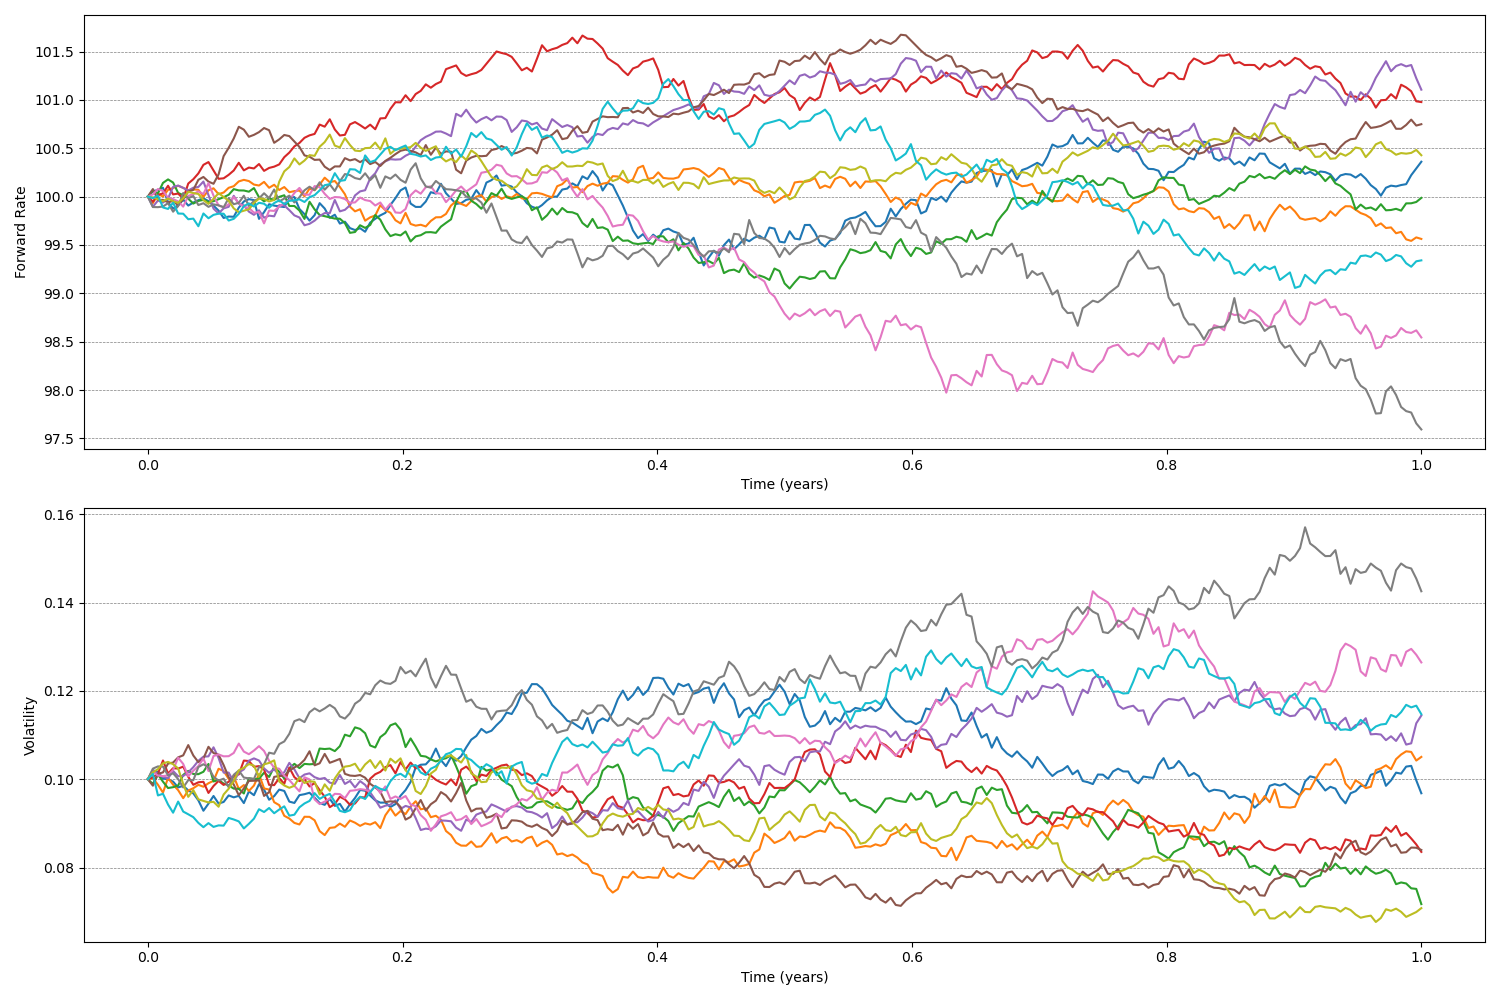
\includegraphics[width=1.\textwidth]{/Users/nannaingemannohrt/Desktop/master_thesis/main/plots/sim_f_and_sigma.png}
    \caption{Ten simulated paths for the forward rate and the volatility in the SABR model.}
    \label{fig:sim_f_and_sigma}
\end{figure}
\noindent
\subsection{SABR Implied Volatility and Option Prices}
Before we are able to move forward with the analysis,
we need to formulate how to determine implied volatility in the SABR model. 
But these calculations are out of the scope for this analysis,
so we will use the formula in the paper Managing Smile Risk 
of Hagen (2002) \cite{Smile}. The paper states that
under the SABR model, the prices of European options 
is given by Black formula in \autoref{sabr1} to \autoref{sabr3}
below
\begin{align}
    V_{\text{call}} &= D(t_{\text{set}})fN(d_1) - KN(d_2)  \label{sabr1}\\
    V_{\text{put}} &= V_{\text{call}} + D(t_{\text{set}})[K - f] \label{sabr2}
\end{align}
with
\begin{equation}
    d_{1,2} = \frac{\log \frac{f}{K} \pm \frac{1}{2}\sigma_B^2 t_{\text{ex}}}{\sigma_B \sqrt{t_{\text{ex}}}}
     \label{sabr3}
\end{equation}
here $t_{\text{set}}$ is the settlement date and $t_{\text{ex}}$ os the exercise date and 
the implied volatility $\sigma_B(f, K)$ is given by
\begin{equation}
    \sigma_B(K, f) = \frac{\alpha}{(fK)^{(1-\beta)/2}} \left\{ 1 + \frac{(1-\beta)^2}{24} \log^2 \frac{f}{K} + \frac{(1-\beta)^4}{1920} \log^4 \frac{f}{K} + \ldots \right\} \left( \frac{z}{x(z)} \right).
    \label{sigma_B}
\end{equation}
where
\begin{align}
    z &= \frac{\nu}{\alpha}(fK)^{(1-\beta)/2} \log \frac{f}{K}, \\
\end{align}
and x(z) is defined by
\begin{align}
    x(z) &= \log \left\{ \frac{\sqrt{1-2\rho z + z^2} + z - \rho}{1 - \rho} \right\}.
\end{align}
For the special case of at-the-money (ATM) options, options strike at $K = f$, this formula reduces to
\begin{equation}
    \sigma_{ATM} = \sigma_B(f, f) = \frac{\alpha}{f^{1-\beta}} \left\{ 1 + \left( \frac{(1-\beta)^2}{24} \frac{\alpha^2}{f^{2-2\beta}} + \frac{\rho \beta \nu}{4} \frac{\alpha}{f^{1-\beta}} + \frac{2-3\rho^2}{24} \nu^2 \right) t_{\text{ex}} + \ldots \right\}.
    \label{sigma_ff}
\end{equation}
\\
So we have that the parameters $\alpha, \beta, \nu$ and $\rho$  in the SABR model is estimated and the implied volatility $\sigma_B$
is a function of the forward price and the strike. Now that we have a simplified formula for the implied 
volatility from the SABR model, we can start analyzing 
how the model works. We will do this by continuing our
analysis with investigating how the different parameters 
affects implied volatility in the SABR model. 


\subsection{Investigating The Parameters of The SABR Model} \label{invest_sabr}
In this Section, we will explore the parameters of the SABR model. This analysis will offer insights into 
how different parameters influence the behavior of implied volatility. We will conduct this investigation using 
the closed-form solution established in the previous Section. Our study will be build on  \autoref{sigma_B} and 
\autoref{sigma_ff}, where we will test various parameter values. To see how changes in the different parameters
affects the implied volatility smile, we fix the values of the parameters during the study. 
The purpose of fixing the values of the parameters, is to isolate the change in the investigated parameter. 
Below in \autoref{tab:parameters} the chosen values of the parameters are listed, together with a short
explain of the parameters. Then the study is performed by changing the parameters one by one, to illustrate the 
isolated effect of the parameters. 
\\
\begin{table}[H]
    \centering
    \begin{tabular}{ccc}
      \toprule
      \textbf{Parameter} & \textbf{Parameter explanation} & \textbf{Value} \\
      \midrule
      \rowcolor{lightgray!40} $F$ & Initial forward rate or asset price & 100 \\
      $T$ & Time to maturity & 1 \\
      \rowcolor{lightgray!40} $K$ & Strike & $K \in (80,120)$ \\
      $\alpha_0$ & Initial level of volatility & 0.1 \\
      \rowcolor{lightgray!40} $\beta$ & Elasticity of the volatility & 0.5 \\
      $\rho$ & Correlation between the asset price and its volatility & -0.4 \\
      \rowcolor{lightgray!40} $\nu$ & Volatility of the volatility parameter & 0.25 \\
      \bottomrule
    \end{tabular}
    \caption{Summary of parameters used for investigating the SABR model}
    \label{tab:parameters}
\end{table}
\noindent
We will start the study with investigating how $\alpha_0$ affects the volatility smile in the SABR model. 
First we note that the fixed value of $\alpha_0$ is $0.1$ Hereafter we adjust the value of $\alpha_0$ to $0.08$ and $0.12$,
where the other parameters are kept fixed as listed in \autoref{tab:parameters} above. So having changed the parameter
up and down from the initial value of $\alpha_0$.
We note that the parameter $\alpha_0$
represents "the initial level of volatility" as it is the starting point for the stochastic volatility process. 
Below in \autoref{fig:alpha} the volatility smile is illustrated for three different value of $\alpha_0$. 
From \autoref{fig:alpha} we see that the up and down movements don't change the shape of the volatility smile, 
it only shifts the volatility smile respectively up and down given the movement in $\alpha_0$.
\begin{figure}[H]
    \centering
    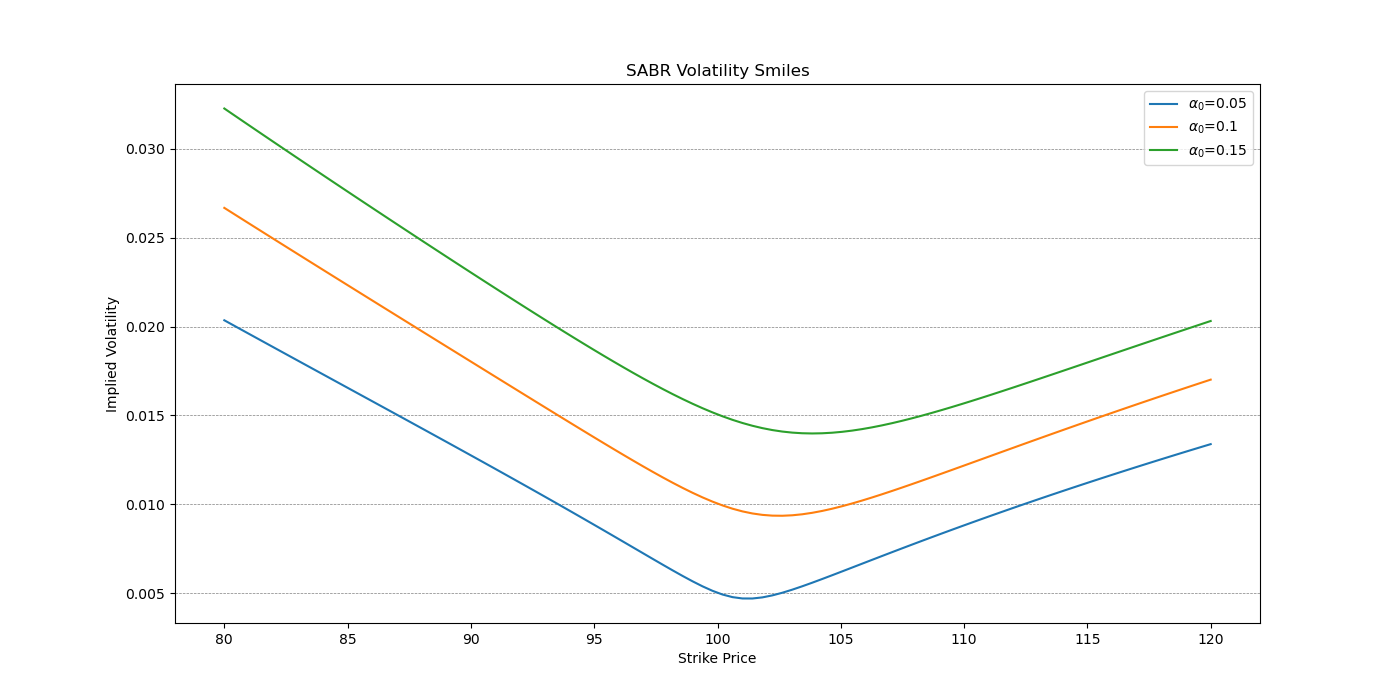
\includegraphics[scale =0.5]{/Users/nannaingemannohrt/Desktop/master_thesis/main/plots/SABR1_alpha.png}
    \caption{SABR model volatility smiles at various $\alpha_0$ levels}
    \label{fig:alpha}
\end{figure}
\noindent
Then we will continue the study of the parameters affects by looking into shift in the $\beta$ value in the SABR model.
Again we shift the value of $\beta$ up and down from the fixed $\beta$ in \autoref{tab:parameters}. So we will look at $\beta$ equal to $0.45$,
$0.5$ (the fix beta) and $0.55$. 
Although not explicitly constrained in the paper Managing Smile Risk 
of Hagen (2002) \cite{Smile} we restrict $\beta$ to the range $[0, 1]$. 
Choosing a $\beta$ less than 0 would lead to an illogical scenario where higher forward prices F result in a smaller 
relative change in the process $F_t$, thus we set the lower limit at $\beta \leq 0$. Similarly, a $\beta$ greater than 1 would 
suggest that the expected deviation from the current state of $F_t$ exceeds the product of volatility and the current 
forward level (times $\alpha_0 \sqrt{t}$), which is also impractical. Therefore, we set the upper limit at $\beta \geq 1$.
\\\\
Below in \autoref{fig:beta} the volatility smile in the SABR model for the different beta values are illustrated.
From \autoref{fig:beta} we see a small effect of the curvature of the volatility smile. We also note that for higher 
beta the shift is larger, than for lower beta. We also note that the change in the beta parameter is more present in 
the left side from of strike value at-the-money (ATM). Other than that we see the same patterns from the change in 
the alpha parameter, namely the up and down shifts in the volatility smile, respectively to the movement in the 
beta parameter.
\begin{figure}[H]
    \centering
    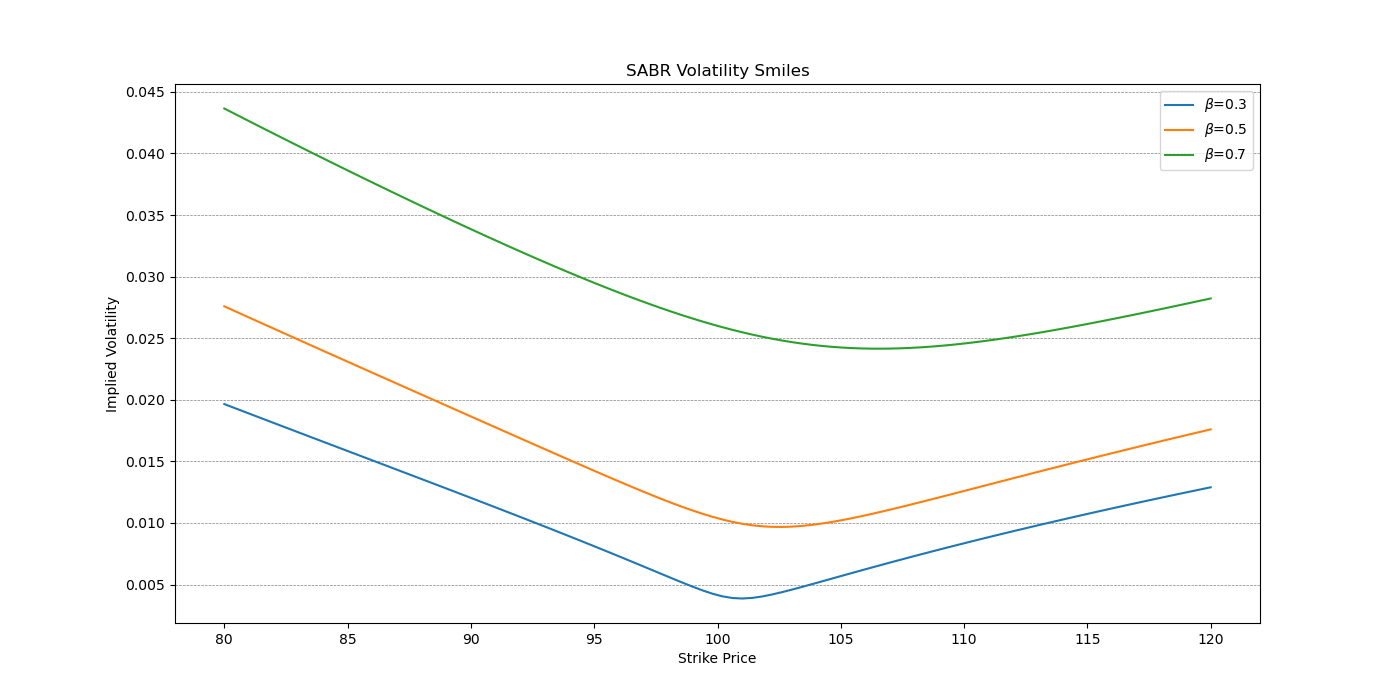
\includegraphics[scale =0.45]{/Users/nannaingemannohrt/Desktop/master_thesis/main/plots/SABR_beta.png}
    \caption{SABR model volatility smiles at various $\beta$ levels}
    \label{fig:beta}
\end{figure}
\noindent
Moving forward we will shift the $\nu$ parameter, which can be describe as the volatility of the volatility parameter.
Again we shift the $\nu$ parameter up and down from the fixed $\nu$ parameter listed in \autoref{tab:parameters}.
The volatility smile calculated from the SABR for the different $\nu$ parameters are illustrated in \autoref{fig:nu} below.
A very clear pattern emerges, namely that the parameter $\nu$ controls the curvature of the volatility smile in
the SABR model. When we looked at the shifts in the beta parameter we made a comment that it made small changes in 
the curvature. But after this part of the analysis, we clearly see that the curvature is determine from the value
of $\nu$. Which makes sense, when we think of the interpretation of the parameter describe before.
We also note that increasing $\nu$  increased the level of the implied volatility for the 
out-of-the-money (OTM) strikes also increase and vise vera.
\\\\
Then we look at the parameter for the correlation between the asset price and its volatility, namely $\rho$.
So we have that $\rho$ is the correlation between to two Wiener process in the SABR model, note
that $\rho$ is bounded and takes values between $-1$ and $1$. In \autoref{fig:rho} the shifted valus of $\rho$
from the fixed value is illustrated. 
We see that higher positive correlations generally show a decreasing trend in implied volatility with an increase in strike price, 
while strong negative correlations can cause the implied volatility to increase with strikes that are in-the-money (ITM).
We alo note that when the correlation is close to zero the smile is more symmetric around the ATM strike. 
So in total we see that the correlation parameter $\rho$ has a significantly affects on the shape and slope of
the volatility smile in the SABR model, and hence on the implied volatilities values.
\begin{figure}[H]
    \centering
    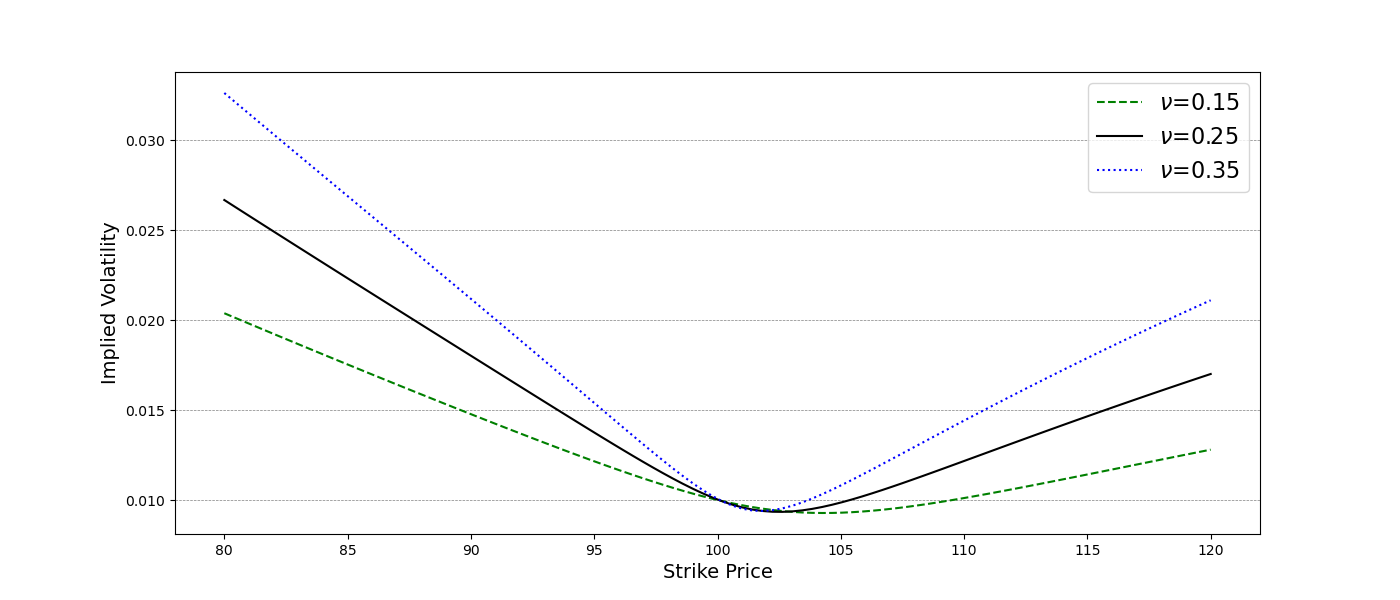
\includegraphics[scale =0.45]{/Users/nannaingemannohrt/Desktop/master_thesis/main/plots/SABR_nu.png}
    \caption{SABR model volatility smiles at various $\nu$ levels}
    \label{fig:nu}
\end{figure}

\begin{figure}[H]
    \centering
    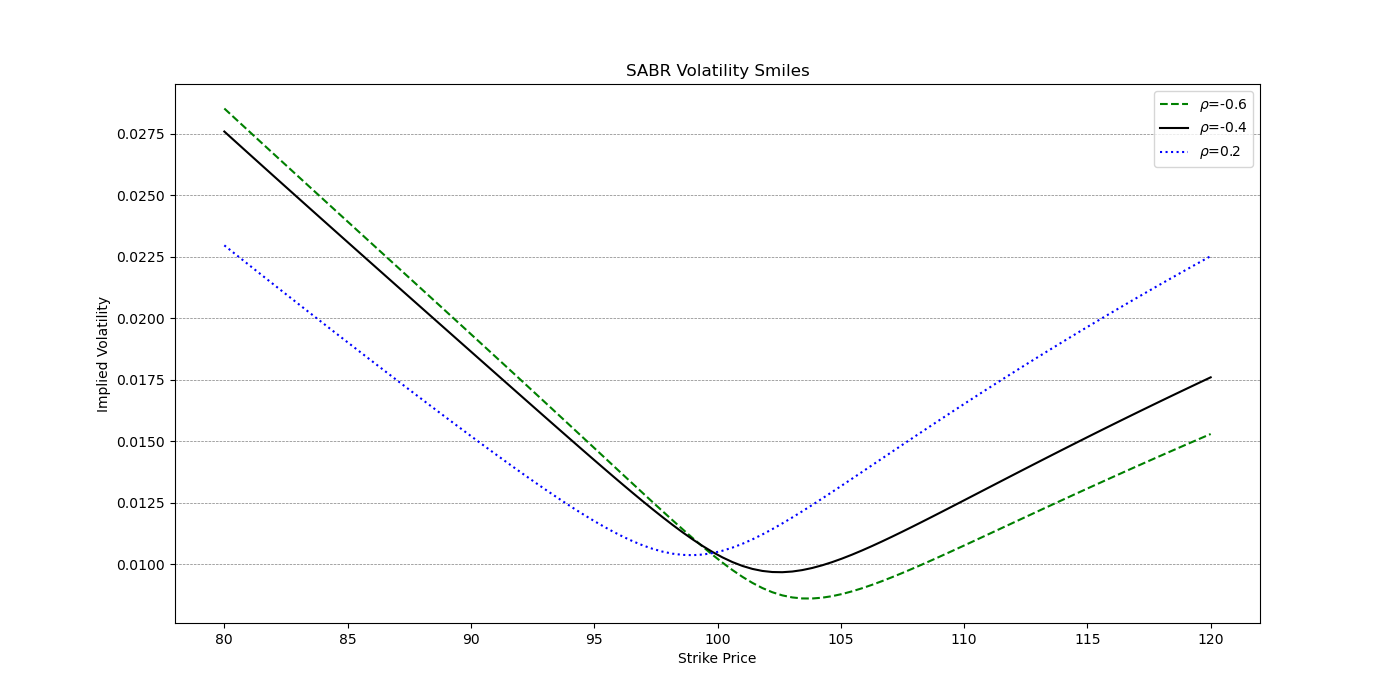
\includegraphics[scale =0.45]{/Users/nannaingemannohrt/Desktop/master_thesis/main/plots/SABR_rho.png}
    \caption{SABR model volatility smiles at various $\rho$ levels}
    \label{fig:rho}
\end{figure}

\begin{figure}[H]
    \centering
    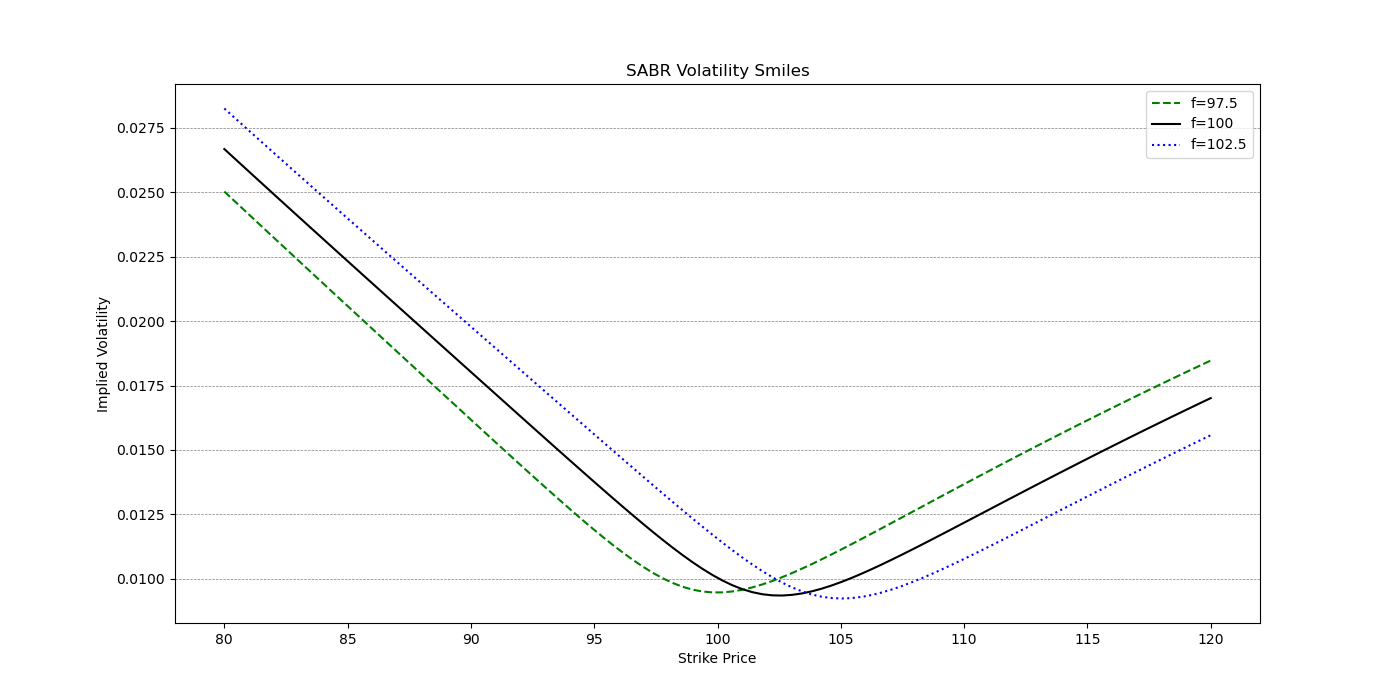
\includegraphics[scale =0.45]{/Users/nannaingemannohrt/Desktop/master_thesis/main/plots/SABR_f.png}
    \caption{SABR model volatility smiles at various F levels}
    \label{fig:f}
\end{figure}
\noindent
Finally we will investigate how the forward price, F, affect the volatility smile in the SABR model. 
The same procedure as for the other parameters will be used. So in \autoref{fig:f} the volatility smile
for the forward prices are illustrated. We see that the slope, shape and curvature is retained, when there
is only change in the forward price. Which is as we expected given how the forward price, F, enters in the closed
solution for the implied volatility in \autoref{sigma_B} and \autoref{sigma_ff}.
\\\\
To summarize this Section provides knowledge of the impact of the various parameters in the closed-form solution
for the implied volatility in the SABR model. This knowledge gives a good idea of how the model works, and 
positions us better to understand estimations of the model. So now we have looked at the closed-form solution and 
are ready for the next step of our analysis which is to look at  estimating the parameters in the SABR model.
\newpage
\subsection{Estimating Parameters in The SABR Model} \label{est_parm_sabr}
In this Section we will look into how we can estimate the parameters in the SABR model.
So we want to estimate $\alpha$, $\beta$, $\rho$ and $\nu$.       
There are different methods for estimating the parameters in the SABR model. 
The various approaches distinguish themselves based on their methods for estimating or selecting $\beta$ and $\alpha$.
$\beta$ may be either set to a predetermined best guess or fitted together with other parameters.
Similarly, $\alpha$ may be estimated using \autoref{sigma_atm} or fitted concurrently with the other parameters.
\\\\
We will apply the approach, where we chose some fixed $\beta$'s and the estimate $\alpha$ using \autoref{sigma_atm}  and the
setup a minimization problem there minimize $\rho$ and $\nu$. We chose this approach since earlier in Chapter \ref{invest_sabr}
we noticed that changes in $\beta$ and $\rho$ gave some of the same effect on the volatility smile. Therefor we chose to fixe  $\beta$, for different
values of $\beta$. Let's then remind yourself of what the change in $\beta$ did to the volatility smile.
We saw that when moving the $\beta$ value op and down, the corresponding change in the volatility smile appeared. 
Then we remind yourself of the dynamic of the forward rate in the SABR model, listed in \autoref{f_dyn}. 
Where we consider the term  $\alpha_t F_t^\beta$ as the total volatility of the forward rate process,
it becomes apparent that decreasing $\beta$ generally amplifies the volatility and vise vera. 
\\\\
Then we consider the minimization problem to estimate the SABR model, where the objective is to align
the market implied volatilities with the SABR model's volatility, which is computed for a 
set of strikes and the current forwards rate for combination of expiry and tenor \cite{Lindstrom}. 
Below the minimization problem is present with the parameters condition we argued for in Chapter \ref{invest_sabr}.
 
\begin{align}
   \min_{\rho, \nu} \sum_{i=0}^{N_k} \Big(\sigma_{\text{B}} - 
    \sigma_{\text{SABR}}(f, \sigma_{\text{ATM}}, k_i, T, \rho, \nu)\Big)^2 \\
    0 \leq \beta \leq 1, \quad -1 \leq \rho \leq 1, \quad 0 \leq \nu, \quad 0 \leq \alpha
\end{align}
There are also different approaches to estimating the $\alpha$ parameter.
To estimate $\alpha$ we will use the method proposed in the paper Managing Smile Risk 
of Hagen (2002) \cite{Smile},
where the ATM SABR-formula is inverted numerically. The ATM SABR-formula is listed in \autoref{sigma_atm} \cite{Smile}.
This is performed in \autoref{sigma_atm} to \autoref{ABC} below.
Another way to estimate $\alpha$ is to solve the 
minimization problem, but this will not be covered in the thesis.

\begin{align}
    \sigma_{\text{ATM}}  & = \frac{\alpha}{f^{1-\beta}} \left\{ 1 +
     \left[ \frac{(1-\beta)^2 \alpha^2}{24 f^{2-2\beta}} + \frac{\rho \beta \nu \alpha}{4 f^{1-\beta}}
      + \frac{(2-3\rho^2) \nu^2}{24} \right] t_{\text{ex}} \right\} \label{sigma_atm} \\
      0 &= A \cdot \alpha^3 + B \cdot \alpha^2 + C \cdot \alpha - \sigma_{\text{ATM}} f^{1-\beta}
\end{align}
where

\begin{align}
    A = \frac{(1-\beta)^2 T}{24 f^{2-2\beta}},
    \quad B = \frac{\rho \beta \nu T}{4 f^{1-\beta}},
    \quad C = \left[ 1 + \frac{2-3\rho^2}{24} \nu^2 \right] t_{\text{ex}} \label{ABC}
\end{align}
Before we are ready to estimate the parameters numerically, let's first take a short look at the required 
data to performed the estimation study. As mentioned we need the current forward rates for any combination 
of expiry and tenor. In this analysis we will consider data where the expiry is ten years and has various tenors 
namely [1Y,2Y,3Y,5Y,7Y,10Y,12Y,15Y,20Y,30Y]. Below in \autoref{tab:farward_parm} the describe forward rates is 
present. To illustrated the development of the forward rates over the different tenors, these are illustrated
in \autoref{fig:forward_plot} below. From the plot we see that the level of the forward rate is higher for
shorter tenors than longer durations tenors.
\\
\begin{table}[H]
    \centering
    \begin{tabular}{ccccccccccc}
      \toprule
      \textbf{ Tenor} & 1Y & 2Y & 3Y & 5Y & 7Y & 10Y & 12Y & 15Y & 20Y & 30Y \\
      \midrule
      \textbf{ Forward rate}&0.2938 & 0.2976 & 0.2996 &0.2992 &0.2943 &0.2840 
      &0.2763 & 0.2654& 0.2517 & 0.2340\\
      \bottomrule
    \end{tabular}
    \caption{Forward rates for ten years to expiry and various tenors. Data source Citi Velocity 21.02.2024}
    \label{tab:farward_parm}
\end{table}
\begin{figure}[H]
    \centering
    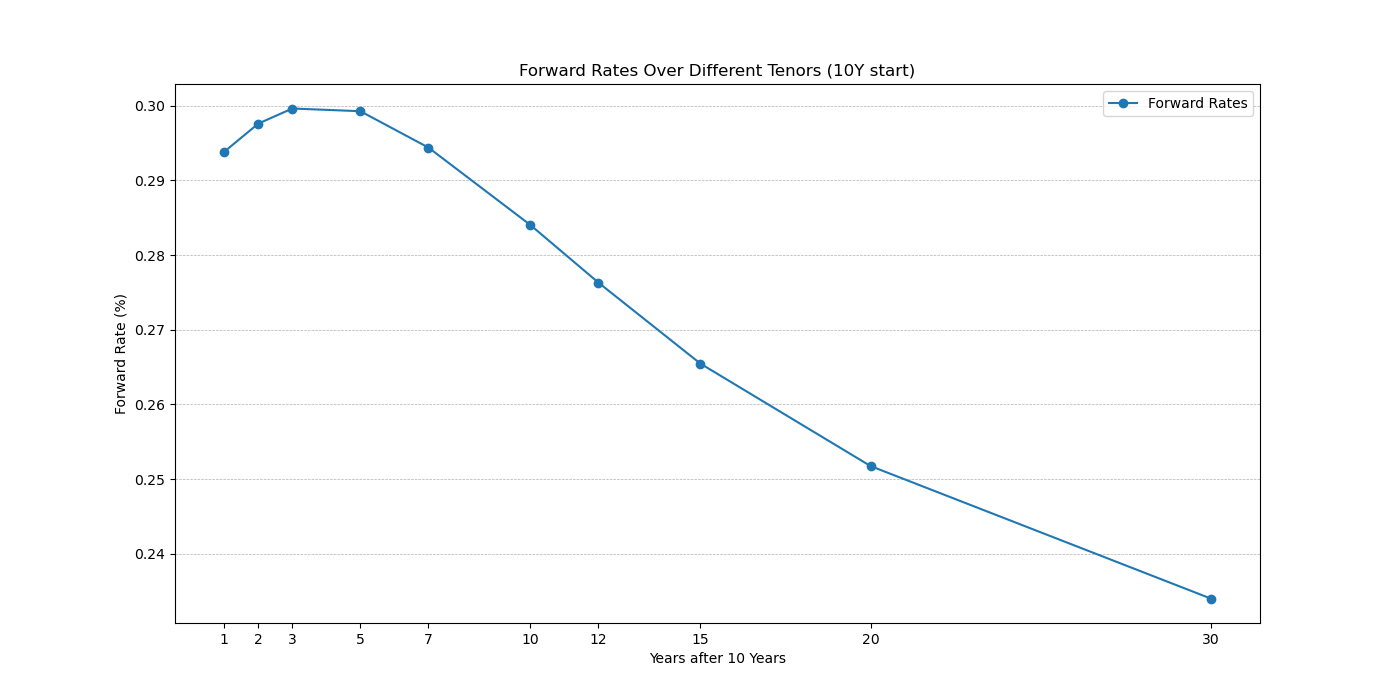
\includegraphics[scale =0.45]{/Users/nannaingemannohrt/Desktop/master_thesis/main/plots/forward_rates.png}
    \caption{Forward rates for ten years to expiry and various tenors. Data source Citi Velocity 21.02.2024}
    \label{fig:forward_plot}
\end{figure}
\noindent
So we have chosen the method where we chose a fixed $\beta$, so we chose the fixed $\beta$'s to be 0.5 and 1.
And then we performed the described estimation for the parameters $\alpha$, $\rho$ and $\nu$. 
This estimation was performed across various combinations of expiry and tenors, 
resulting in two separate tables that display the estimated parameters when $\beta$ is fixed at either 0.5 or 1. 
The estimated values for $\alpha$, $\rho$, and $\nu$, with $\beta$ fixed at 0.5, are presented in \autoref{tab:beta_0.5}. 
Similarly, the values for when $\beta$ is fixed at 1 are shown in \autoref{tab:beta_1}.
\\\\
\\\\
Lets first comment on the estimated values in  \autoref{tab:beta_0.5}, where $\beta=0.5$.
The estimated parameters show generally moderate values for $\alpha$ across different tenor-expiry combinations, 
with a slight tendency to increase for longer expiries. The $\rho$ estimated values are predominantly positive, 
suggesting that higher rates correlate with higher volatility. Finally $\nu$  estimated values are high, 
indicating substantial volatility skew, which might suggest expectations of greater changes in 
rate movements over these periods. Then lets comment on the estimated values in \autoref{tab:beta_1}, where $\beta=1$.
In this case, the estimated $\alpha$ values are relatively higher compared to $\beta$ = 0.5, suggesting increased erratic behavior in volatility 
for these scenarios. The $\rho$ estimated  values are also positive but exhibit a wider range across different tenors and expiries. 
The estimated $\nu$ values remain high, reinforcing the presence of a significant volatility skew.
\\
\begin{table}[H]
    \centering
    \begin{tabular}{cccc}
      \toprule
      \textbf{Expiry x Tenor } & \textbf{$\hat{\alpha}$} & \textbf{$\hat{\rho}$}  & \textbf{$\hat{\nu}$} \\
      \midrule
      \rowcolor{lightgray!40}  10Y x 1Y &0.2526 & 0.3711 & 3.8123 \\
      10Y x 2Y &0.2516 & 0.3546 & 3.7993 \\
      \rowcolor{lightgray!40}  10Y x 3Y  &0.2460 & 0.3367 & 3.7752 \\
      10Y x 5Y &0.2394 & 0.3030 & 3.7173 \\
      \rowcolor{lightgray!40} 10Y x 7Y &0.2278 & 0.2762 & 3.7246 \\
      10Y x 10Y &0.2130& 0.2368 & 3.73220 \\
      \rowcolor{lightgray!40}  10Y x 12Y &0.2129 & 0.2461& 3.445 \\
      10Y x 15Y &0.2007 & 0.2201 & 3.6347 \\
      \rowcolor{lightgray!40} 10Y x 20Y &0.1939 & 0.2048 & 3.5607 \\
      10Y x 30Y &0.1881 & 0.1942 & 3.4496 \\
      \bottomrule
    \end{tabular}
    \caption{$\hat{\alpha}$, $\hat{\rho}$ and $\hat{\nu}$ for fixed $\beta$ = 0.5, using the SABR model.}
    \label{tab:beta_0.5}
\end{table}
\noindent

\begin{table}[H]
    \centering
    \begin{tabular}{cccc}
      \toprule
      \textbf{Expiry x Tenor} & \textbf{$\hat{\alpha}$} & \textbf{$\hat{\rho}$}  & \textbf{$\hat{\nu}$}\\
      \midrule
      \rowcolor{lightgray!40} 10Y x 1Y &0.4577 & 0.3114 & 3.6282 \\
      10Y x 2Y  &0.4535 & 0.2947 & 3.6284 \\
      \rowcolor{lightgray!40} 10Y x 3Y  &0.4426 & 0.2772 & 3.6199\\
      10Y x 5Y  &0.4320 & 0.2429 & 3.5869 \\
      \rowcolor{lightgray!40} 10Y x 7Y  &0.4153 & 0.2176 & 3.6137 \\
      10Y x 10Y &0.3962& 0.1799 & 3.6463 \\
      \rowcolor{lightgray!40} 10Y x 12Y &0.4420 & 0.1762 & 3.3525\\
      10Y x 15Y & 0.3865 & 0.1623 & 3.3560 \\
      \rowcolor{lightgray!40} 10Y x 20Y &0.3838 & 0.1456 & 3.4955 \\
      10Y x 30Y &0.3867 & 0.1221 & 3.3960 \\
      \bottomrule
    \end{tabular}
    \caption{$\hat{\alpha}$, $\hat{\rho}$ and $\hat{\nu}$ for fixed $\beta$ = 1, using the SABR model.}
    \label{tab:beta_1}
\end{table}
\noindent
The analysis of the SABR model parameters, specifically at fixed $\beta$ values of 0.5 and 1, 
reveals distinctive volatility dynamics and correlation structures across various tenor-expiry combinations. 
At both $\beta$ values, the presence of a positive $\rho$ indicates that rate increases are likely correlated with heightened volatility.
The notable distinctions at $\beta$ = 1 are the higher $\alpha$ and $\nu$ values, suggesting a more erratic behavior and pronounced 
skewness in volatility. These characteristics are particularly significant for pricing and risk management in scenarios 
anticipating substantial rate dynamics. The insights garnered from this analysis are crucial for financial institutions and 
investors involved in hedging, pricing, or trading derivatives influenced by these model dynamics.
\\\\
To end this section we will look at estimated parameters despited by the volatility smile. 
We chose to look a the volatility smile, for estimated values where $\beta$ was fixed to be 0.5. 
Since this is the most common choice for $\beta$. We despited the combination where the tenor is 10 years, i large format in 
\autoref{fig:10y_plot_smile} below and all combined of the swaption volatility smile with expiry in 10 years, and the 
various tenors are despited in \autoref{fig:10Y1Y_} to \autoref{fig:10Y10Y_} below. 
From \autoref{fig:10y_plot_smile}  we se that estimated volatility smile fits the market data good, which make sense from 
how we estimated the parameters to find the volatility smile. We note that estimated values for $\nu$ in both 
\autoref{tab:beta_0.5} and \autoref{tab:beta_1}, are relative high. But this align with the steepness or level we see the in the 
volatility smile in the market data. The volatility smile tends to be more convex when $\nu$ is large and this is clearly 
the case here. This tendency appearers in  most of the volatility smile despited in \autoref{fig:10Y1Y_} to \autoref{fig:10Y10Y_}.
But again we also see for the tenor-expiry combination for longer tenor, has not the same steepness in the level in 
the volatility smile. For the longer dated tenor combination we see a more symmetric volatility smile around the
ATM strike. We also note the the changes in the volatility smile i larger for the OTM strike, than for the ITM strikes. 
\\\\
Then we should ask yourself how does the  steepness or level we see the in the 
volatility smile in the market data affects the price of a swaption. When we are determine swaption we should also consider 
with sensitivities there are related to the price of the swaption. The above analysis pointing at there could 
be a sensitive related to $\nu$. Therefor the next step in the analysis is to look closer at the models sensitivities. 
But first a look at how swaption prices change over various tenors in Chapter \ref{swaption_price_sec}.

\begin{figure}[H]
    \centering
    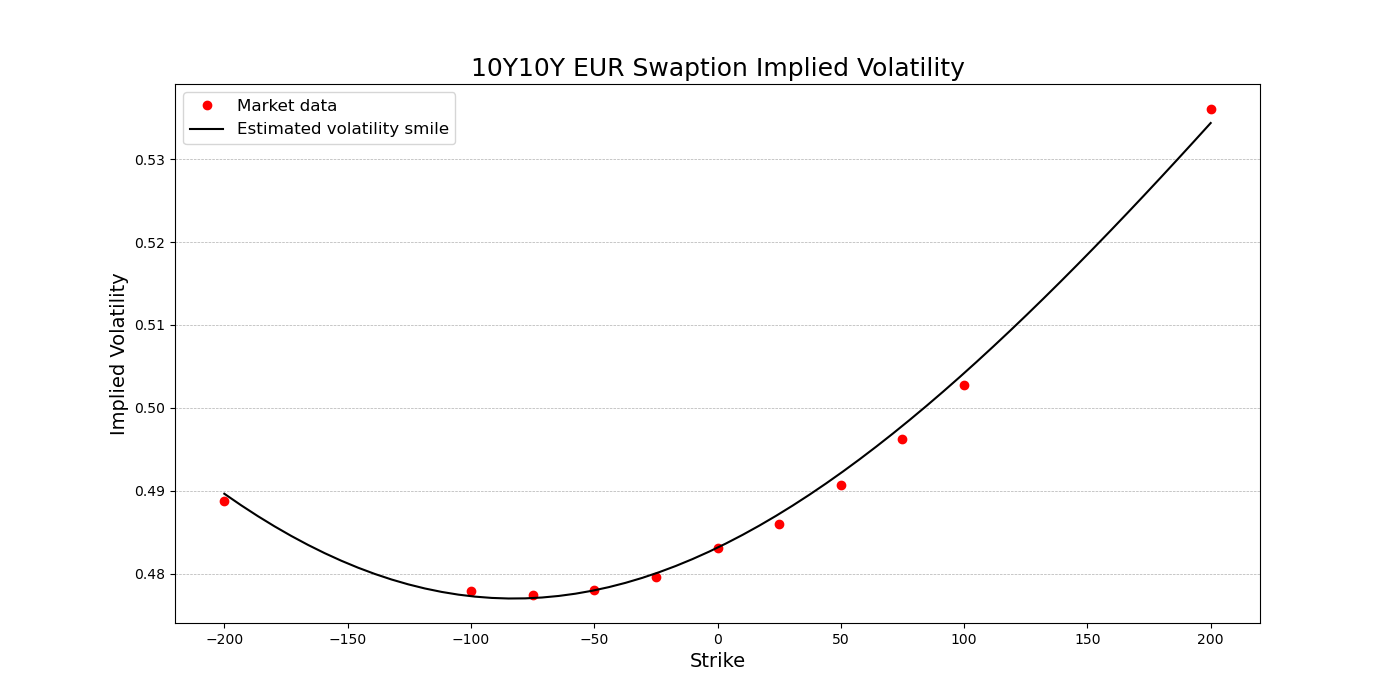
\includegraphics[scale = 0.5]{/Users/nannaingemannohrt/Desktop/master_thesis/main/plots/10Y10Y_est.png}
    \caption{Estimated implied volatility smile for a 10Y10Y EUR swaption using the SABR model. 
    \\ Data source Citi Velocity 21.02.2024}
    \label{fig:10y_plot_smile}
\end{figure}
\noindent


\begin{figure}[htbp]
    \centering
    \begin{subfigure}{0.43\textwidth}
        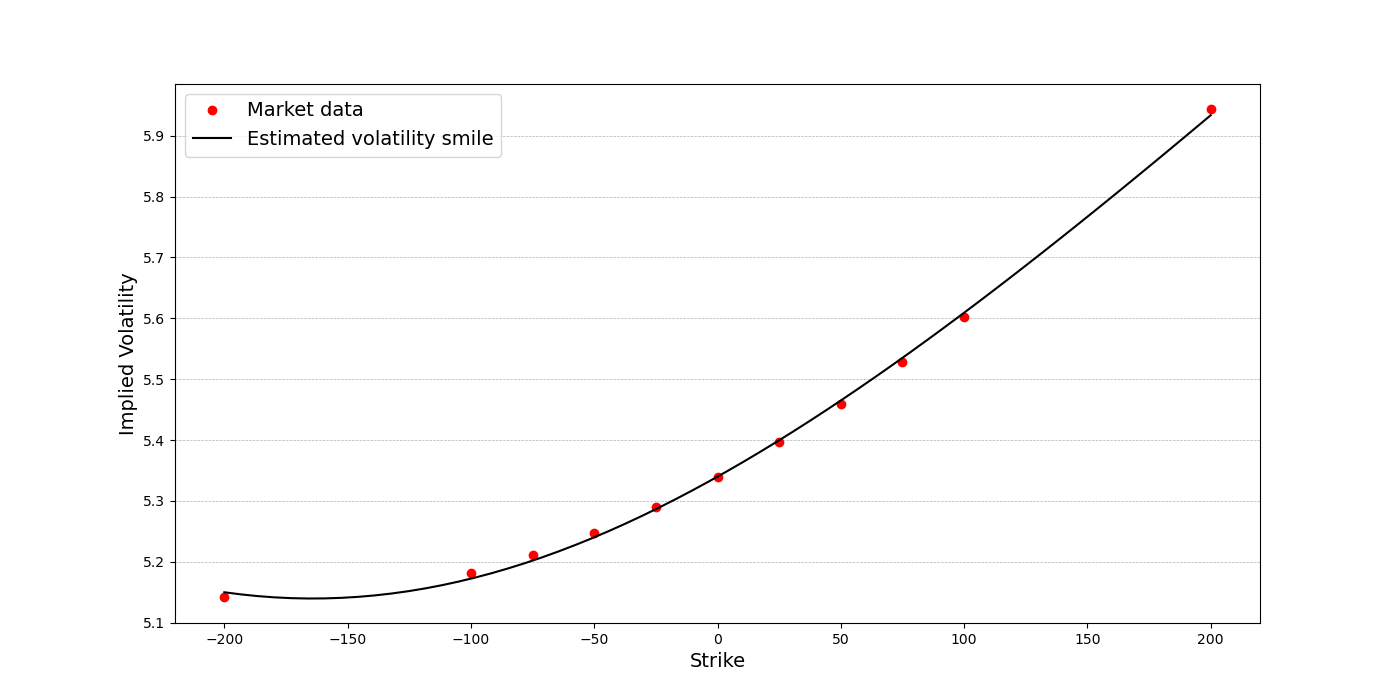
\includegraphics[scale =0.22]{/Users/nannaingemannohrt/Desktop/master_thesis/main/plots/10Y1Y_est.png}
        \caption{Volatility Surface EUR swaption 10Y1Y}
        \label{fig:10Y1Y_}
    \end{subfigure}\hfill
    \begin{subfigure}{0.43
        \textwidth}
        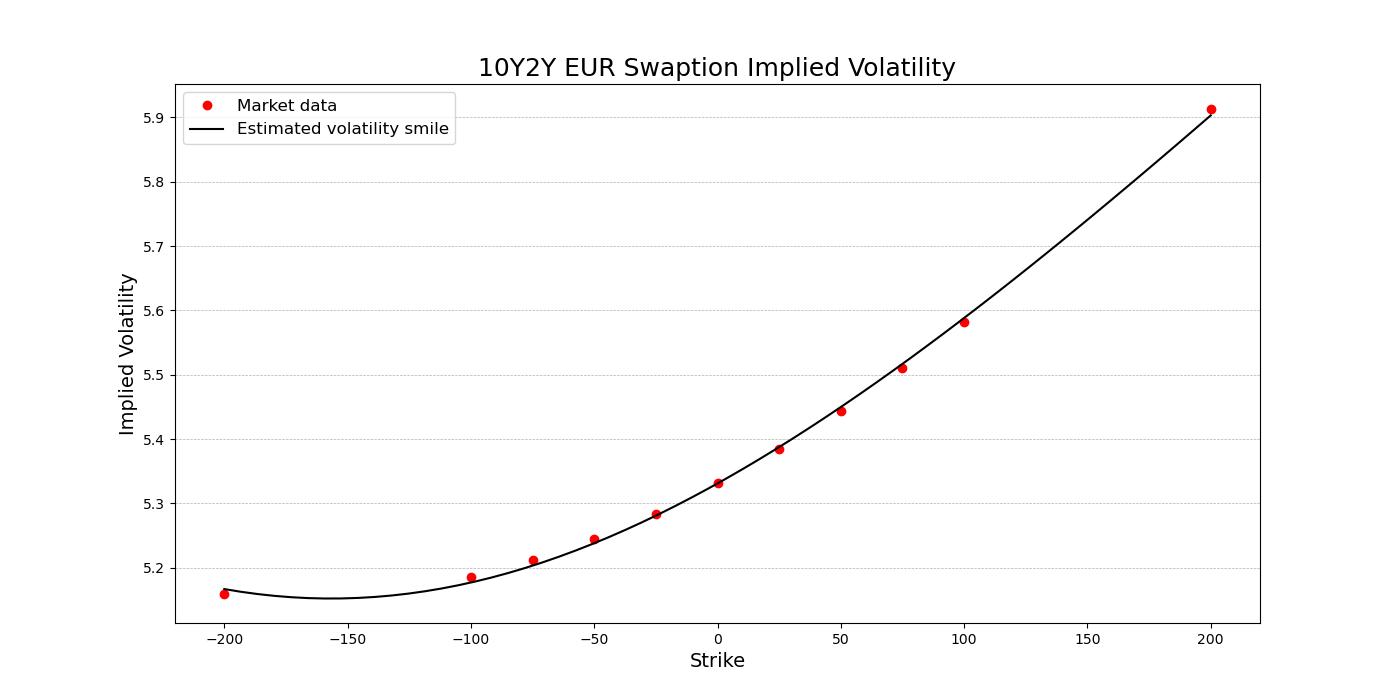
\includegraphics[scale =0.22]{/Users/nannaingemannohrt/Desktop/master_thesis/main/plots/10Y2Y_est.png}
        \caption{Volatility Surface EUR swaption 10Y2Y}
        \label{fig:10Y2Y_}
    \end{subfigure}
    \begin{subfigure}{0.43\textwidth}
        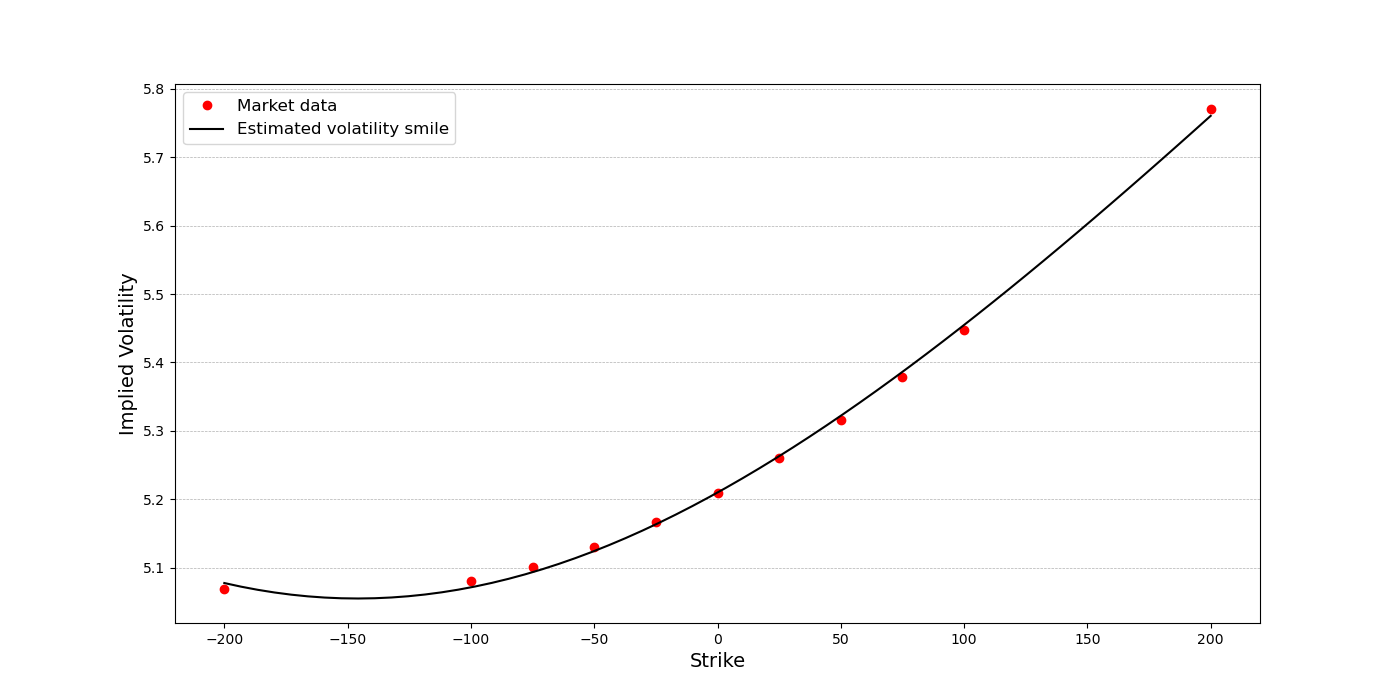
\includegraphics[scale =0.22]{/Users/nannaingemannohrt/Desktop/master_thesis/main/plots/10Y3Y_est.png}
        \caption{Volatility Surface EUR swaption 10Y3Y}
        \label{fig:10Y3Y_}
    \end{subfigure}\hfill
    \begin{subfigure}{0.43\textwidth}
        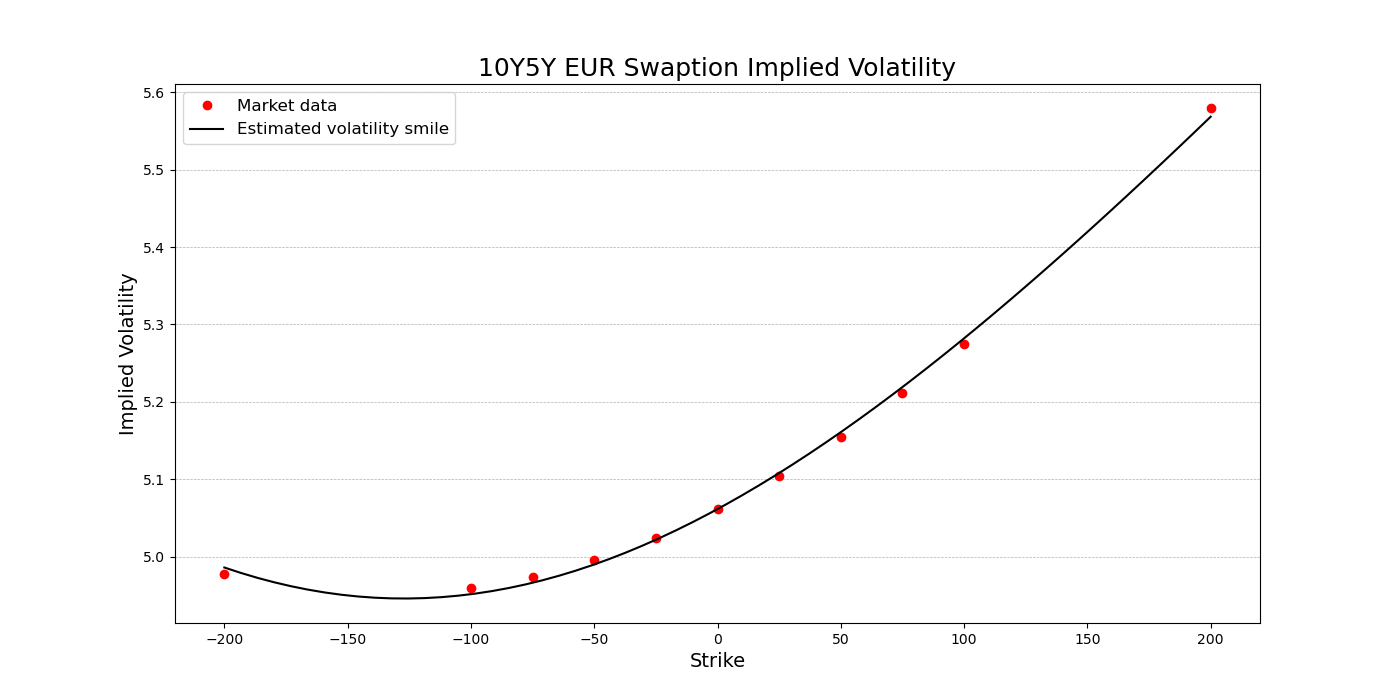
\includegraphics[scale =0.22]{/Users/nannaingemannohrt/Desktop/master_thesis/main/plots/10Y5Y_est.png}
        \caption{Volatility Surface EUR swaption 10Y5Y}
        \label{fig:10Y5Y_}
    \end{subfigure}
    \begin{subfigure}{0.43\textwidth}
        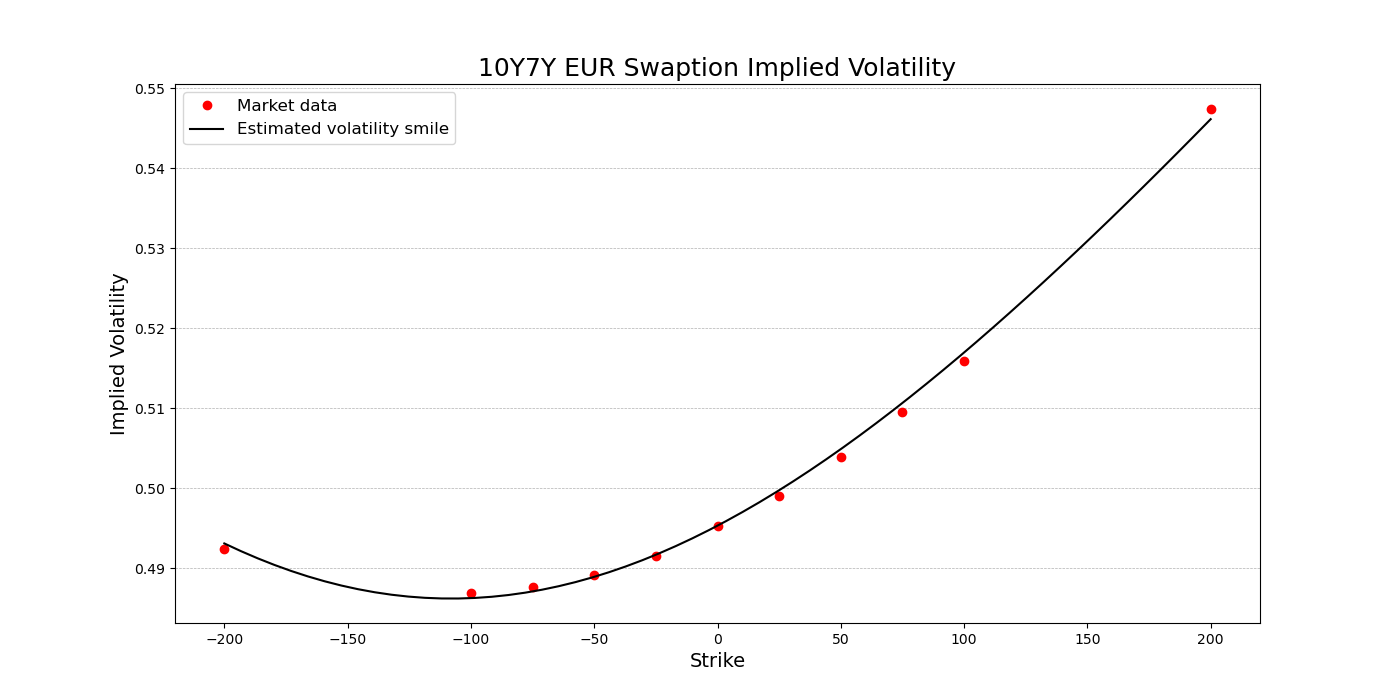
\includegraphics[scale =0.22]{/Users/nannaingemannohrt/Desktop/master_thesis/main/plots/10Y7Y_est.png}
        \caption{Volatility Surface EUR swaption 10Y7Y}
        \label{fig:10Y7Y_}
    \end{subfigure}\hfill
    \begin{subfigure}{0.43\textwidth}
        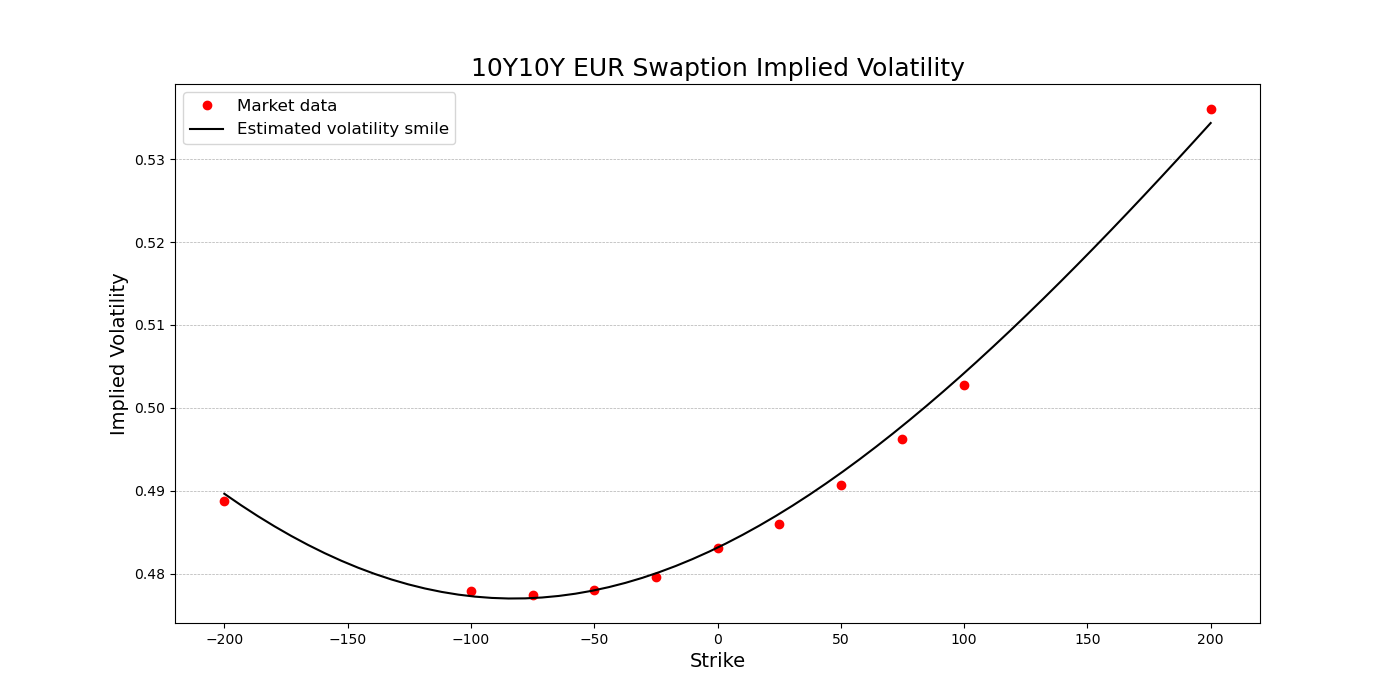
\includegraphics[scale =0.22]{/Users/nannaingemannohrt/Desktop/master_thesis/main/plots/10Y10Y_est.png}
        \caption{Volatility Surface EUR swaption 10Y10Y}
        \label{fig:10Y10Y_}
    \end{subfigure}

    \begin{subfigure}{0.43\textwidth}
        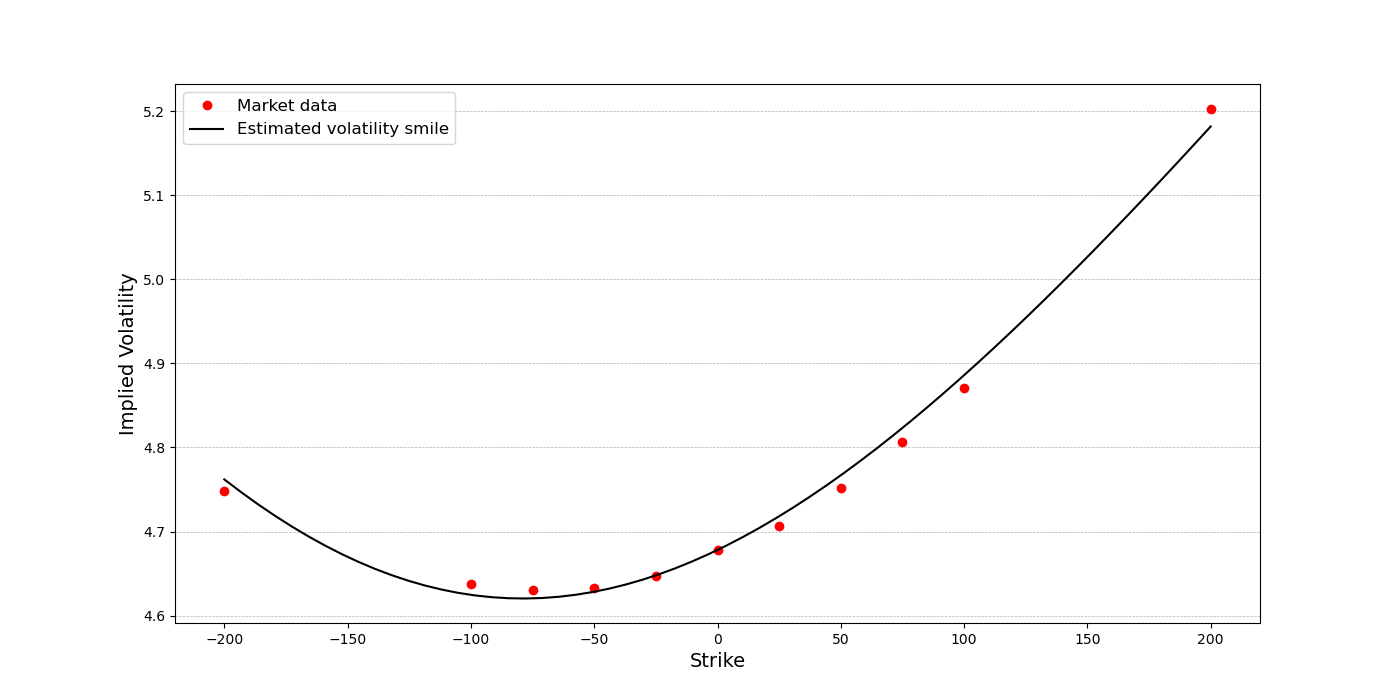
\includegraphics[scale =0.22]{/Users/nannaingemannohrt/Desktop/master_thesis/main/plots/10Y12Y_est.png}
        \caption{Volatility Surface EUR swaption 10Y12Y}
        \label{fig:10Y12Y_}
    \end{subfigure}\hfill
    \begin{subfigure}{0.43\textwidth}
        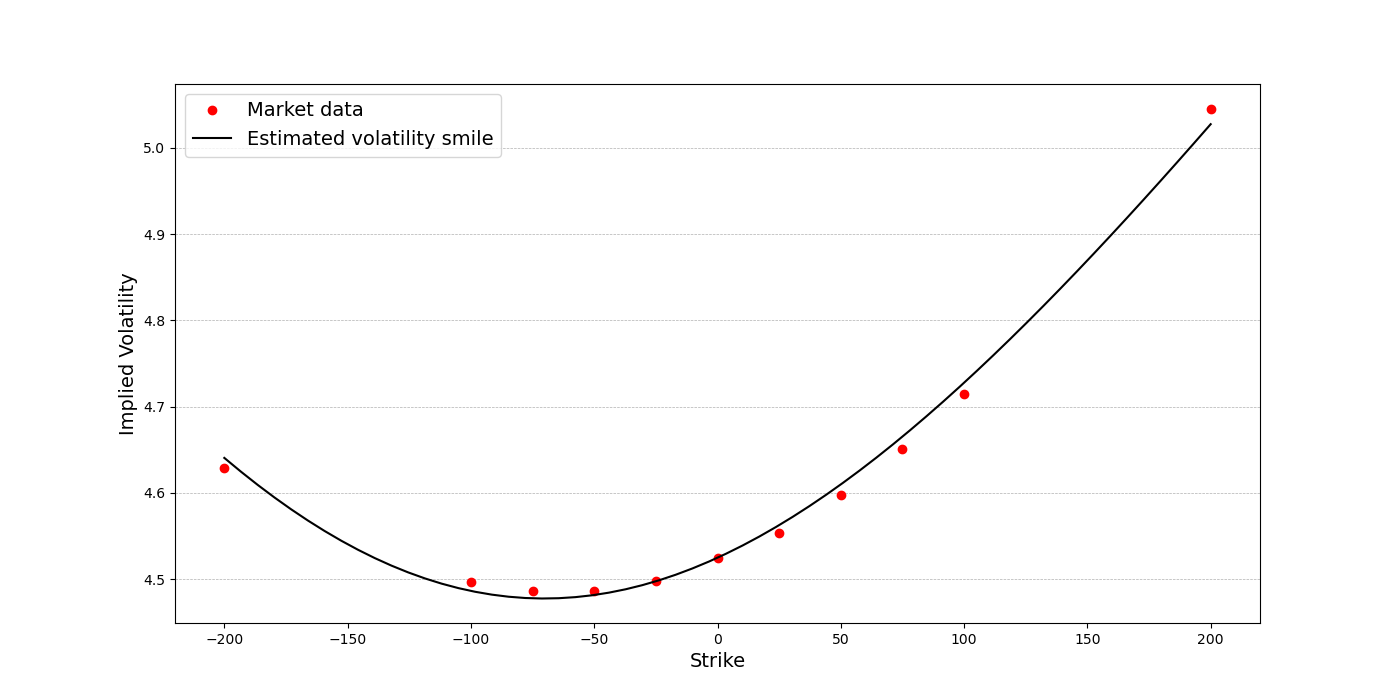
\includegraphics[scale =0.22]{/Users/nannaingemannohrt/Desktop/master_thesis/main/plots/10Y15Y_est.png}
        \caption{Volatility Surface EUR swaption 10Y15Y}
        \label{fig:10Y15Y_}
    \end{subfigure}
    \begin{subfigure}{0.43\textwidth}
        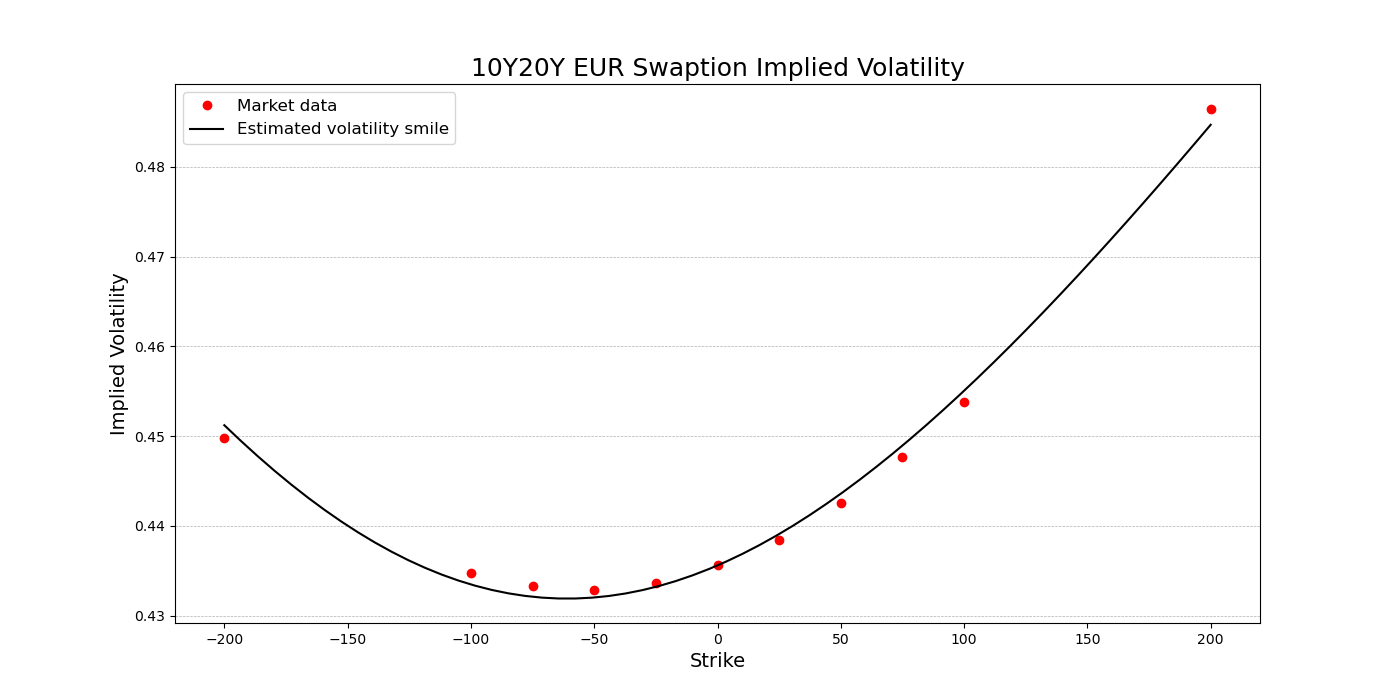
\includegraphics[scale =0.22]{/Users/nannaingemannohrt/Desktop/master_thesis/main/plots/10Y20Y_est.png}
        \caption{Volatility Surface EUR swaption 10Y20Y}
        \label{fig:10Y20Y_}
    \end{subfigure}\hfill
    \begin{subfigure}{0.43\textwidth}
        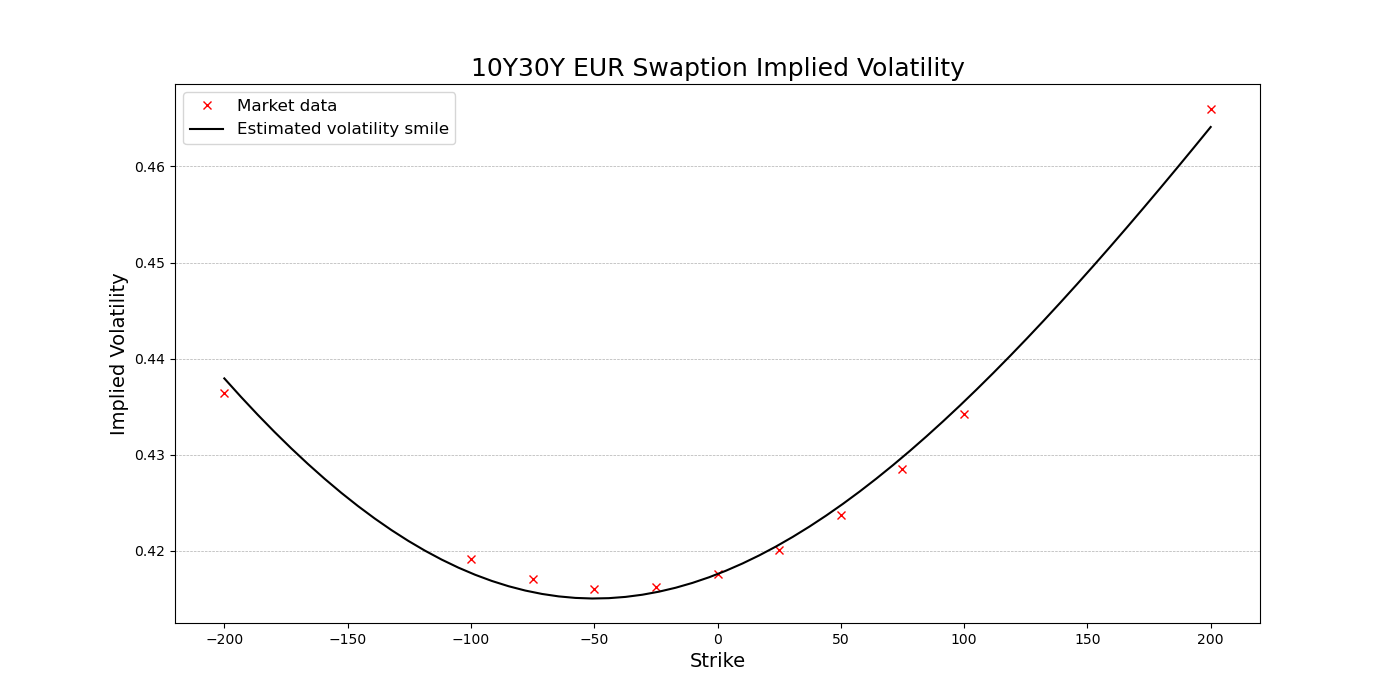
\includegraphics[scale =0.22]{/Users/nannaingemannohrt/Desktop/master_thesis/main/plots/10Y30Y_est.png}
        \caption{Volatility Surface EUR swaption 10Y30Y}
        \label{fig:10Y30Y_}
    \end{subfigure}

\end{figure}   
\newpage
\section{Swaption Pricing} \label{swaption_price_sec}
Now we hav seen that the implied volatility can change over various tenors. 
Therefore it is important to be aware of how the volatility affect the market.
And thereby which asset there maybe will perform in different situations i the market,
due to high or low volatility, inflation and other factor the can influence the market.
When it comes to swaption and other asset the volatility also has
a remarkable determination of the price of the asset. 
\\\\
In the Section \ref{invest_sabr} we learned how the different parameters in the 
SABR model affects the implied volatility in swaption. 
Where in Section \ref{est_parm_sabr} we estimated the parameters in the SABR model. 
From these Sections we saw some clear coincidence between the level of a given parameter
and the effect on the implied volatility. 
This implied volatility determine from the SABR model, is then used to price swaption using the 
Black-Scholes model. 
Therefor we have computed the prices for swaption with a fixed expiry at 10 years and for various tenors. 
The price are ATM, which means that, F, the forward rate is equal to, K, 
the strike (the rate of the underlying asset). 
\\\\
Below in \autoref{tab:swaption_price_atm} the calculated prices for the various swaption 
using the describe method is listed. 
The prices are ATM prices for a fixed tenor at 10 yeas and for various tenors. 
To illustrated the development of the price over the different tenors, 
the swaption price is despited below in  \autoref{fig:swaption_price_atm}.
\begin{table}[H]
  \centering
  \begin{tabular}{ccccccccccc}
    \toprule
    \textbf{ Tenor} & 1Y & 2Y & 3Y & 5Y & 7Y & 10Y & 12Y & 15Y & 20Y & 30Y \\
    \midrule
    \textbf{ Swaption price }&0.1334 & 0.1351 & 0.1360 &0.1358  &0.1336  &0.1289
    &0.1254& 0.1205 & 0.1143 & 0.1062 \\
    \bottomrule
  \end{tabular}
  \caption{ATM swaption price in basis point for a 10 years fixed expiry and various tenors.
  Data source  \\ Citi Velocity 21.02.2024}
  \label{tab:swaption_price_atm}
\end{table}
\noindent
\autoref{fig:swaption_price_atm} shows a decreasing tends in swaptions prices as the tenor increases,
starting off relatively flat in the shorter durations tenors (1 to 5 years) and then 
descending more steeply from around the 5 year tenor. 
The pattern in the graph indicates that the longer the duration of the swaptions tenor, 
the lower the cost to enter into one. A swaption is essentially an option that grants the 
holder the right, but not the obligation, to initiate a swap agreement with specific terms at a future date. 
The graph shows that swaption prices are relatively stable for shorter tenors and begin to 
decrease more noticeably for durations extending beyond 5 years. 
This flattening in the initial period could be due to more predictable or stable interest 
rate expectations in the near term. Conversely, the significant price drop for longer 
tenors might suggest greater uncertainty or a reduced interest in securing rate locks for extended periods.
\begin{figure}[H]
    \centering
    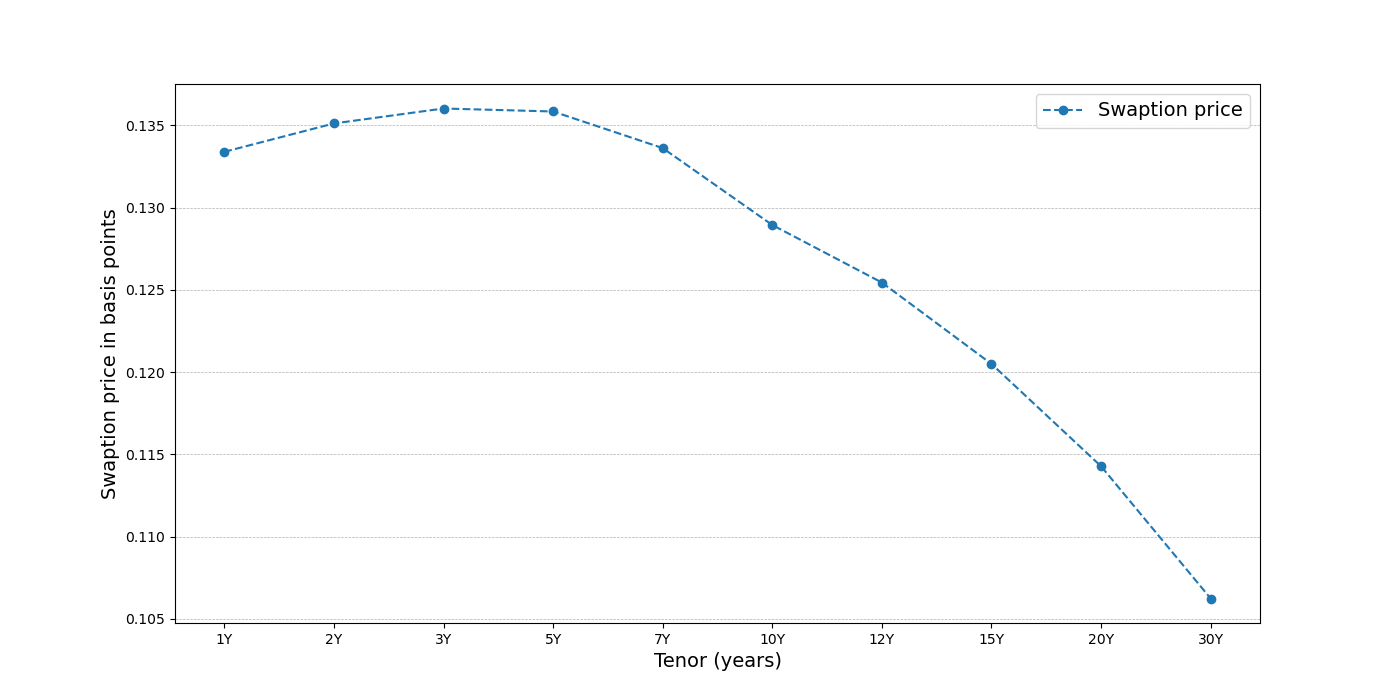
\includegraphics[scale = 0.5]{/Users/nannaingemannohrt/Desktop/master_thesis/main/plots/swaption_price_atm.png}
    \caption{ATM swaption price in basis point for a 10 years fixed expiry and various tenors.
    Data source  \\ Citi Velocity 21.02.2024}
    \label{fig:swaption_price_atm}
\end{figure}
\noindent
So in other words \autoref{fig:swaption_price_atm}  could indicate that swaptions with a lower is less
volatile than longer duration tenor swaption. This could be exampled by that in finance we will 
expected short terms interest rate to behave like the short rate in the Vasicek model for example. 
We in the Vasicek model we learned that the short rate tend to a mean reverting level. 
So there will not be expected larger fluctuations on short term, but we don't know how the market is in 
30 years. But if we compare the shape of the calculated swaptions price in \autoref{fig:swaption_price_atm} 
to shape of the forward \autoref{fig:forward_plot}. We see that the same tendency in the slope 
is represented. Hence the market expectations the that the forward is lower for longer duration tenor, 
than for short duration tenor. 
\\\\
But as mentioned there are other factor there affect the price of a swaption than the level of the forward. 
Also the other parameters in the SABR model also affect the swaption price indirect, 
since the parameter effect the implied volatility. 
So as promise Chapter \ref{risk_mang} we will look into the sensitivities in the SABR model.

\newpage
\section{Risk Related to The SABR Model} \label{risk_mang}
In this Chapter risk related to the SARB model will be covered. 
This will be a adding to the investigation of the parameters in the SABR model.
We will start this Chapter by  reminding yourself of the value for
a European call swaption according to the SABR model. 
Then the Chapter will continuing covering the related risk, also called referred to as sensitives in 
the SABR model. 
\\\\
So du to the examination of the Black Scholes model we have that \cite{Smile}
\begin{align}
    V_{\text{call}} &= D(t_{\text{set}})fN(d_1) - KN(d_2) \label{V_call} 
\end{align}
with
\begin{equation}
    d_{1,2} = \frac{\log \frac{f}{K} \pm \frac{1}{2}\sigma_B^2 t_{\text{ex}}}{\sigma_B \sqrt{t_{\text{ex}}}}
\end{equation}
where $t_{\text{set}}$ is the settlement date and $t_{\text{ex}}$ is the exercise date.
According to the SABR model, the value of a call is 
\begin{align}
    V_{\text{call}}= BS(f, K, \sigma_{\text{B}}(K,f),t_{\text{ex}})
\end{align}
with  
\begin{align}
    \sigma_{\text{B}}(K,f) \equiv \sigma_{\text{B}}(K,f;\alpha, \beta, \rho, \nu)
\end{align}
where the implied volatility $\sigma_{\text{B}}(K,f) $ is given as below
\begin{equation}
    \sigma_B(K, f) = \frac{\alpha}{(fK)^{(1-\beta)/2}} \left\{ 1 + \frac{(1-\beta)^2}{24} \log^2 \frac{f}{K} + \frac{(1-\beta)^4}{1920} \log^4 \frac{f}{K} + \ldots \right\} \left( \frac{z}{x(z)} \right)
    \label{eg_2}
\end{equation}
where
\begin{align}
    z &= \frac{\nu}{\alpha}(fK)^{(1-\beta)/2} \log \frac{f}{K}, \\
\end{align}
and x(z) is defined by
\begin{align}
    x(z) &= \log \left\{ \frac{\sqrt{1-2\rho z + z^2} + z - \rho}{1 - \rho} \right\}
\end{align}
For the special case of ATM options, options strike at $K = f$, this formula reduces to
\begin{equation}
    \sigma_{ATM} = \sigma_B(f, f) = \frac{\alpha}{f^{1-\beta}} \left\{ 1 + \left( \frac{(1-\beta)^2}{24} \frac{\alpha^2}{f^{2-2\beta}} + \frac{\rho \beta \nu}{4} \frac{\alpha}{f^{1-\beta}} + \frac{2-3\rho^2}{24} \nu^2 \right) t_{\text{ex}} + \ldots \right\}
    \label{sigma_ff_risk}
\end{equation}
\\\\
Lets then remind yourself of the interpretation of the parameters in the SABR model. 
\begin{itemize}
    \item $F_0$ \text{---} Initial forward rate or asset price.
    \item $\alpha_0$ \text{---} Initial volatility.
    \item $\beta$ \text{---} Elasticity parameter.
    \item $\nu$ \text{---} Volatility of the volatility parameter.
    \item $\rho$ \text{---} Correlation between the asset price and its volatility.
\end{itemize}
\noindent
So new we are ready to look at the risk related to the SABR model.
We will cover some different types of risk, namely vega, vanna, volga and delta risk. 
The various types of risk, are related to the parameters in the SABR. 
From your analysis of SABR model we argued that it is common practice, 
to fixed beta. Hence we will not look into any risk related to the beta parameter. 
But all the other parameters risk will be study. 
\\\\
During the examination of the risk related to the SABR will will look at 
the derivatives with respect to the different parameters. 
First we will look at the vega risk, which is the risk related to the $\alpha$ parameter. 
Hence it is also the risk related to the changes in the  volatility.
\\\\
From differentiating \autoref{V_call} with respect to $\alpha$ we have that
\begin{align}
    \frac{\partial V_{\text{call}}}{\partial \alpha} = 
    \frac{\partial \text{BS}}{\partial \sigma_B} \cdot \frac{\partial 
    \sigma_B(K, f; \alpha, \beta, \nu)}{\partial \alpha}
\end{align}
When taking about the risk related to the change in volatility, $\alpha$, 
the risk changes by a unit amount. We also note the it is common used finance to 
scale vega, so it represents the change in value when the AMT volatility change by a unit amount \cite{Smile}.
Then we note that 
\begin{align}
    \delta  \cdot \sigma_{\text{ATM}} =
     \Big(\frac{\partial \sigma_{\text{ATM}}}{\partial \alpha} \Big) \cdot \delta \alpha \label{eg_1}
\end{align}
where $\delta$ represents the changes. Due to \autoref{eg_1} we can write the vega risk as below
\begin{align}
    \text{vega} \equiv  \frac{\partial V_{\text{call}}}{\partial \alpha} 
   = \frac{\frac{\partial \sigma_B(K, f; \alpha, \beta, \nu)}{\partial \alpha}}
    {\frac{\partial \sigma_{\text{ATM}}(f; \alpha, \beta, \nu)}{\partial \alpha}} \label{eg_3}
\end{align}
 where we have that $\sigma_{\text{ATM}}(f) = \sigma_{\text{B}} (f,f)$  is given as listed in \autoref{sigma_ff_risk}
 above. 
Then we note that  $\frac{\partial \sigma_B}{\partial \alpha} \approx \frac{ \sigma_B}{ \alpha}$ 
and $\frac{\partial \sigma_{\text{ATM}}}{\partial \alpha} \approx \frac{ \sigma_{\text{ATM}}}{\alpha}$,
hence the vega risk can be expressed as 
\begin{align}
\text{vega} \approx \frac{\partial \text{BS}}{\partial \sigma_B} \cdot
 \frac{\sigma_B(K,f)}{\sigma_{\text{ATM}}(f)} \cdot \frac{\partial \text{BS}}{\partial \sigma_B} 
 \cdot \frac{\sigma_B(K,f)}{\sigma_B(f,f)}
\end{align}
So when we work with the SABR model,
the vega risks for a swaption at various strike prices are calculated by adjusting the implied volatility at each strike 
K. This adjustment is proportional to the existing implied volatility 
$\sigma_B(K,f)$
at that strike. In this way, using \autoref{eg_3}, we adjust the
volatility curve in a proportional manner, rather than shifting 
it uniformly, allowing us to more accurately calculate the total
vega risk for a portfolio of options.
\\\\
The we  remind yourself of how $\rho$ and $\nu$ are determine in the SABR model.
We learned that $\rho$ and $\nu$ are determine by fitting the implied volatility
surface observed in the market. But there are also risk related to these 
to parameters. So now we will look into the vanna and volga risk. 
First we note that the vanna risk in the SABR model, is related 
to the  parameter $\rho$. Secondly the volga risk is related
to the $\nu$ risk. The lingo of volga comes from volatility of gamma
\cite{Smile}. Gamma measure the convexity of a derivative's value in relation to the underlying asset. 
\\\\
Then lets look at how the two risk is determined. 
\begin{align*}
    \text{vanna} &= \frac{\partial V_{\text{call}}}{\partial \rho} = \frac{\partial BS}{\partial \sigma_B} \frac{\partial \sigma_B(K, f; \alpha, \beta, \nu)}{\partial \rho} \\
    \text{volga} &= \frac{\partial V_{\text{call}}}{\partial \nu} = \frac{\partial BS}{\partial \sigma_B} \frac{\partial \sigma_B(K, f; \alpha, \beta, \nu)}{\partial \nu}
\end{align*}
\\
Then we remind yourself of the interpretation of $\rho$,
which was the correlation between the asset price and the its 
volatility. Which make since since the vanna risk express
the risk ro the skew increase. In other word the vanna risk 
measures the sensitives of an option  vega to change in 
the underlying asset price. Next we will cover the volga risk.
The volga risk is related to the $\nu$ parameter in the SABR model. 
The volga risk expresses the risk to the smile shape and curvature,
which we also saw during the investigating of the SABR model. 
This is also consistent with the interpretation of the $\nu$ parameter. 
Exactly that $\nu$ is the volatility of the volatility parameter $\alpha$.
\newpage
\noindent
Finally we will look at the delta risk, we will denoted
the delta risk $\Delta$. The delta risk is related to f, the 
forward rate or the price of the underlying asset. 
During the investigating of the SABR model, we made
some choice regrading the determining of the alpha parameter.
This choice also effect the delta risk. So we note that
we chose the approach of determine the alpha, from solve the
$\sigma_{\text{ATM}}$, where $\sigma_{\text{ATM}}$ is given as 
listed in \autoref{sigma_ff_risk} above. 
Then we differentiating with respect to f, to obtain the delta risk. 
\begin{align}
    \Delta = \frac{\partial \text{BS}}{\partial f} +
     \frac{\partial \text{BS}}{\partial \sigma_\beta} 
     \Big({\frac{\partial \sigma_\beta(K; f, \alpha, \beta, \rho, \nu)}
     {\partial f}  + \frac{\partial \sigma_\beta(K; f, \alpha, \beta,
     \rho, \nu)}{\partial \alpha} 
     \frac{\partial \sigma(\text{ATM}, f)}{\partial f}}\Big)
\end{align}
The first term represents the ordinary delta risk calculated from 
the Black's model. The second term adds the SABR model's
 specific adjustment for the change in implied volatility, 
$\sigma_B$, caused by changes in the forward price f.
The last term represents the adjustment needed to maintain a constant 
$\sigma_{\text{ATM}}$ while f changes.
We also note that the last term will be zero, if $\beta=1$ \cite{Smile}.
\\\\
Now we have covered all the risk or sensitives related to the SABR model. 
The tends we saw during the investigating of the SABR model, reflects
the same patterns regrading the various risk related to the model. 
\newpage
\section{Conclusion}
\newpage
\begin{appendices} 
 \chapter{One-Factor Short-Rate model}\label{appendices}
   
 As mentioned we will now look a the formula for pricing bonds using the Vasicek model. We consider a zero coupon bond
 with maturity T and at time t the price is given as in \autoref{price_zcb_vas} below \cite{Bjork}.
 \begin{align}
     P(t,T) &= A(t,T) e^{-rB(t,T)} 
     \label{price_zcb_vas} 
 \end{align}
 \\\\
 Then we find the partial derivatives with respect to $r$ and $t$ of the zero coupon bond listed in \autoref{price_zcb_vas}.
 \begin{align*}
     \frac{\partial P}{\partial t} &= \frac{\partial}{\partial t} (Ae^{-rB}) 
     = e^{-rB} \frac{\partial A}{\partial t} + Ae^{-rB} \frac{\partial}{\partial t} (-rB) \\
     &= e^{-rB} \frac{\partial A}{\partial t} - rAe^{-rB} \frac{\partial B}{\partial t} = 
     - \frac{P}{A} \frac{\partial A}{\partial t} - rP \frac{\partial B}{\partial t}
     \\\\
     \frac{\partial P}{\partial r} &= \frac{\partial}{\partial r} (Ae^{-rB}) 
     = Ae^{-rB} \frac{\partial}{\partial r} (-rB) = -PB 
     \\\\
     \frac{\partial^2 P}{\partial r^2} &= \frac{\partial}{\partial r} (-PB) = -B \frac{\partial}{\partial r} (P) = PB^2
 \end{align*}
 Then by applying Ito's lemma \cite{Bjork} and inserting the derivatives with respect to $r$ and $t$ we found above as well as
  the formula for the short rate in the Vasicek model present in \autoref{vas_dyn1} we obtain the following
 \begin{align*}
     dP(t,T) &= \frac{\partial P}{\partial t} dt + \frac{\partial P}{\partial r} dr 
     + \frac{1}{2} \frac{\partial^2 P}{\partial r^2} dr^2 \\
     dP(t,T) &= \left( \frac{P}{A} \frac{\partial A}{\partial t} - rP \frac{\partial B}{\partial t} \right) dt 
     + (-PB) dr + \frac{1}{2} (PB^2) dr^2 \\
     \frac{dP}{P} &= \left( \frac{1}{A} \frac{\partial A}{\partial t} - r \frac{\partial B}{\partial t} \right) dt 
     - B dr + \frac{1}{2} B^2 dr^2 \\
     \frac{dP}{P} &= \left( \frac{1}{A} \frac{\partial A}{\partial t} - r \frac{\partial B}{\partial t} \right) dt
      - B(\kappa \theta dt - \kappa r dt + \sigma dW_t) + \frac{1}{2} B^2 \sigma^2 dt\\
     \frac{dP}{P} &= \left( \frac{1}{A} \frac{\partial A}{\partial t} - r \frac{\partial B}{\partial t} 
     - \kappa \theta B + \kappa r B + \frac{1}{2} B^2 \sigma^2 \right) dt - \sigma B dW_t \\
 \end{align*}
 Under the risk neutral measure, the expected return of the bond must be equal to the risk free rate. Thus we have that
 \begin{align*}
     r  &= \frac{1}{A} \frac{\partial A}{\partial t} - r \frac{\partial B}{\partial t} - \kappa \theta B 
     + \kappa r B + \frac{1}{2} B^2 \sigma^2  \\
     r \left( 1 + \frac{\partial B}{\partial t} - \kappa B \right) & =\frac{1}{A} \frac{\partial A}{\partial t} 
     - \kappa \theta B + \frac{1}{2} B^2 \sigma^2 
 \end{align*}
 Since this holds for all values of $r$, which does not feature in the left hand side, we deduce that
 \begin{align}
     0 &= \frac{1}{A} \frac{\partial A}{\partial t} - \kappa \theta B + \frac{1}{2} B^2 \sigma^2 \label{equal_zero2}\\
     0 &=1 + \frac{\partial B}{\partial t} - \kappa B \label{equal_zero}
 \end{align}
 Considering that the price of zero coupon bond at maturity $P(T,T)=1$, the function $P=A e^{-rB}$ suggests $B(T,T)=0$
 and $A(T,T)=0$. By then applying the integrating factor to the \autoref{equal_zero}, reorganizing and integrating
 form t to T, we obtain
 \begin{align}
    0 &= 1 + \frac{\partial B}{\partial t} - \kappa B \nonumber  \\
    0 &= e^{-\kappa t} + e^{-\kappa t} \frac{\partial B}{\partial t} - e^{-\kappa t} \kappa B \nonumber \\
    -e^{-\kappa t} &= e^{-\kappa t} \frac{\partial B}{\partial t} - e^{-\kappa t} \kappa B  \nonumber \\
    -e^{-\kappa t} dt &= d \left( e^{-\kappa t} B(t, T) \right) \nonumber \\
    - \int_{t}^{T} e^{-\kappa u} du &= \int_{t}^{T} d \left( e^{-\kappa t} B(t, T) \right) \nonumber  \\
    \frac{1}{\kappa} \left( e^{-\kappa T} - e^{-\kappa t} \right) &= e^{-\kappa T} B(T, T) - e^{-\kappa t} B(t, T)\nonumber  \\
    B(t,T) & =\frac{1}{\kappa} \left( 1 - e^{-\kappa (T-t)} \right)  
 \end{align}
 Finally  by substituting into \autoref{equal_zero2} and integrating we get that
 \begin{align}
     0 &=\frac{1}{A} \frac{\partial A}{\partial t} - \kappa \theta B + \frac{1}{2} B^2 \sigma^2 \nonumber \\
     0 &= \frac{1}{A} \frac{\partial A}{\partial t} - \kappa \theta \left( \frac{1 - e^{-\kappa(T-t)}}{\kappa}
     \right) + \frac{\sigma^2}{2\kappa^2} \left( 1 - e^{-\kappa(T-t)} \right)^2 \nonumber \\
     0 &=  \frac{1}{A} \frac{\partial A}{\partial t} - \theta \left( 1 - e^{-\kappa(T-t)} \right) 
     + \frac{\sigma^2}{2\kappa^2} \left( 1 + e^{-2\kappa(T-t)} - 2e^{-\kappa(T-t)} \right)\nonumber \\
     \frac{1}{A} \frac{\partial A}{\partial t} &€= \theta \left( 1 - e^{-\kappa(T-t)} \right) 
     - \frac{\sigma^2}{2\kappa^2} \left( 1 + e^{-2\kappa(T-t)} - 2e^{-\kappa(T-t)} \right) \nonumber\\
     \int_{t}^{T} \frac{dA(u, T)}{A(u, T)} &= \theta \int_{t}^{T} \left(1 - e^{-\kappa(T-u)}\right) du 
     - \frac{\sigma^2}{2\kappa^2} \int_{t}^{T} \left(1 + e^{-2\kappa(T-u)} - 2e^{-\kappa(T-u)}\right) du \nonumber\\
     \ln A(T, T) - \ln A(t, T) &= \theta (T - t) - \theta \left(\frac{1 - e^{-\kappa(T-t)}}{\kappa} \right)
     - \frac{\sigma^2}{2\kappa^2} \left( (T - t) + \left(\frac{1 - e^{-2\kappa(T-t)}}{2\kappa}\right) 
     - 2\frac{1 - e^{-\kappa(T-t)}}{\kappa}\right) \nonumber\\
     -\ln A(t, T) &= \theta (T - t) - \theta \left(\frac{1 - e^{-\kappa(T-u)}}{\kappa} \right)
     - \frac{\sigma^2}{4\kappa^3} \left(2\kappa (T - t) + 1 - e^{-2\kappa(T-t)} - 4 + 4e^{-\kappa(T-t)}\right) \nonumber\\
     -\ln A(t, T) &= \theta (T - t) - \theta \left(\frac{1 - e^{-\kappa(T-u)}}{\kappa} \right)
     - \frac{\sigma^2}{4\kappa^3} \left(2\kappa (T - t) - \left(1 + e^{-2\kappa(T-t)} 
     - 2e^{-\kappa(T-t)}\right) - 2 + 2e^{-\kappa(T-t)}\right) \nonumber\\
     -\ln A(t, T) &= \theta (T - t) - \theta \left(\frac{1 - e^{-\kappa(T-u)}}{\kappa}\right) - \frac{\sigma^2}{2 \kappa^2}
     \left((T-t)- \frac{1-e^{-\kappa(T-t)}}{\kappa}\right) + \frac{\sigma^2}{4 {\kappa}^3}\left(1-e^{-\kappa(T-t)}\right)^2 \nonumber\\
     \ln A(t, T) &= \left(\theta -\frac{\sigma^2}{2\kappa^2}\right) \left(\frac{1-e^{-\kappa(T-u)}}{\kappa}-(T-t)\right)
     -\frac{\sigma^2}{4 \kappa}\left(\frac{1-e^{-\kappa(T-t)}}{\kappa}\right)^2 \nonumber\\
     A(t,T)&= \exp \Biggl\{\left(\theta-\frac{\sigma^2}{2 \kappa^2}\right)\left(\frac{1-e^{-\kappa(T-u)}}{\kappa}-(T-t)\right)
     -\frac{\sigma^2}{4 \kappa}\left(\frac{1-e^{-\kappa(T-t)}}{\kappa}\right)^2 \Biggr\} 
 \end{align}
 \\\\
  Combining this we get the formula for pricing bonds using the Vasicek model, which present 
  in Proposition \autoref{prop 5} below. 
 
 \begin{proposition}
     \label{prop 5}
     \textbf{(The Vasicek term structure)} In the Vasicek model, bond prices are given by
  \begin{align}
     P(t,T) &= A(t,T) e^{-rB(t,T)} 
 \end{align}
 where
 \begin{align*}
     A(t,T)&= \exp \Biggl\{\left(\theta-\frac{\sigma^2}{2 \kappa^2}\right)\left(\frac{1-e^{-\kappa(T-u)}}{\kappa}-(T-t)\right)
     -\frac{\sigma^2}{4 \kappa}\left(\frac{1-e^{-\kappa(T-t)}}{\kappa}\right)^2 \Biggr\} \\
     B(t,T) & =\frac{1}{\kappa} \left( 1 - e^{-\kappa (T-t)} \right)  
 \end{align*}
 \cite{Bjork}
 \end{proposition}
 \noindent
\end{appendices}
    
\newpage
\clearpage
\addcontentsline{toc}{section}{References}

\begin{thebibliography}{25}
 \bibitem{Bjork}
 Björk, Tomas,
 \emph{Arbitrage Theory in Continuous Time},
 Oxford, fourth edition, 2020

 \bibitem{Hull}
Hull, John C., 
\emph{Options, futures, and other derivatives},
Pearson, eleventh edition, global edition, 2022

\bibitem{Lindstrøm}
Linderstrøm, Martin Dalskov, 
\emph{Fixed Income Derivatives Lecture Notes},
2013
 
\end{thebibliography}

\bibliography{tesis} 
\newpage
\addcontentsline{toc}{section}{Code}
\subsection*{Code} 

\end{document}